%%%%%%%%%%%%%%%%%%%%%%%%% INTRO %%%%%%%%%%%%%%%%%%%%%%%%%%%%


\section{Introduction}
\def\stmt{$A$}
% \def\stmt{$\phi$}


\commentout{%oli-v1
	The ability to articulate a \emph{degree of confidence}
	% (or the opposite: a degree of uncertainty)
	is a critical aspect of representing knowledge.
	There are
	many well-established ways to quantify (un)certinaty \parencite[\S2]{halpern2017reasoning},
		and chief among them is probability.
	While ``confidence'' can be coherently read in probabilistic terms,
		such usage may shadow another important concept.
	This paper details a different conception that arises when updating beliefs.
	As we shall see, this notion of confidence
	complements traditional representations of uncertainty (such as probability),
	and moreover unifies several different concepts across AI.
}

% What should it mean to say that one has a high degree of confidence in a statement $\phi$? 
% It is often taken to mean that we think $\phi$ is likely.
What does it mean to have a high degree of confidence in a statement $\phi$? 
It is often taken to mean that $\phi$ is likely.
% This paper details a different conception that arises when updating beliefs.
% As we shall see, this notion of confidence
% complements traditional representations of uncertainty (such as probability),
We argue that there is a related conception of confidence that arises when learning---one that complements likelihood and, moreover, unifies several different concepts in the literature.
% Here we argue that there is a related but more useful way of defining confidence, which complements notions like probability and, moreover, unifies several different concepts in the literature.
%oli4
% For us, confidence is a measure of \emph{trust}, rather than likelihood.
This kind of confidence is a measure of \emph{trust}, rather than likelihood.
% We are intereted in the conception of confidence as measuring \emph{trust}, rather than likelihood.
% In more detail, the {degree of confidence} that one has in a piece
The degree of confidence one places in a piece of information $\phi$
%is a number  $\chi \in [\bot,\top]$ that
quantifies how seriously to take $\phi$ in updating one's beliefs.
So at one extreme,
if we observe $\phi$ but have no confidence in it,
we should not change our beliefs at all;
at the other, if we have full confidence in $\phi$,
 we should fully incorporate it into our beliefs.

% If our belief state is a probability measure $\Pr$ and $\phi$ is an event, for example, then fully incorporating $\phi$ amounts to conditioning $\Pr$ on it.
\begin{example}
	% [Linear interpolation]
 \label{ex:prob-simple}
%oli2: alternate presentation that makes it clear that \Pr | \phi is
%   a conditional measure; it is uncommon to write it this way
%   in modern ML, and may be confusing without explanation.
% Suppose our belief state is a probability measure, and $\phi$ is an event.
% A full-confidence update then amounts to conditioning on $\phi$, after which $\phi$ has probability 1, and so cannot be further incorporated.
Suppose our prior belief state is a probability measure $\Pr$, and $\phi$ is an event.
A full-confidence update then amounts to conditioning on $\phi$ (i.e., adopting the belief state $\Pr\mid\phi$), after which $\phi$ has probability 1 and cannot be further incorporated.
Here is one obvious way
to describe intermediate degrees of confidence:
if we learn $\phi$ with confidence
$\alpha \in [0,1]$
%oli2:
% and start with prior probability $\Pr$, then we end up with the
and start with prior $\Pr$, then we end up with the
%oli1: I agree that this notation is nicer, but these days it
% is also much less standard than p(X) and p(X|\phi). In particular,
% my ML friends who work with applied probability a lot do not understand
% how to parse  "\Pr | \phi".
posterior $(1-\alpha)\Pr + \alpha (\Pr\mid \phi)$.
%
Thus, having high confidence in $\phi$ leads to posterior beliefs that give $\phi$
high probability.
The converse is false, however, so
confidence and probability can be quite different.
If an untrusted source tells us $\phi$ which we already happen to believe,
then our prior assigns $\phi$ high probability,
we learn $\phi$ with low confidence,
and our posterior beliefs still give $\phi$ high probability.
%joe1: I don't know what "more independent" means
% Confidence and prior probability are even more independent:
% Also,
% Confidence is even less coupled to prior probability:
% Prior probabilty is further decoupled from confidence:
% Prior probability ($\Pr(\phi)$) and confidence $\chi$ are further decoupled:
%joe3: Cut the rest of the paragraph. In the previous you argued that confidence is not the same as posterior probability. Now you suddenly bring in prior probability. The story here is completely unclear.
%oli3: Right, I previously argued that confidence is not the same as posterior probability. Now I'm saying it's not the same as prior probability either.  (and indeed, it's even less related.) Why is the story unclear?
\commentout{
Prior probability and confidence are further decoupled:
if we learn a surprising fact $\phi$ from a trusted source, we have high confidence in $\phi$ despite it having low prior probability.
}
% This leads to an important observation: one's confidence in $\phi$ is not a feature of one's prior probability at all.
% Thus, confidence in $\phi$ is independent from $\Pr(\phi)$.
\end{example}


Confidence allows us to be uncertain about observations,
which is quite different in principle from making observations that are uncertain.
% There are well established ways of doing this, such as Jeffrey's rule
% \emph{Jeffrey's rule} \parencite{} is a well-established way of handling the latter, and so it is often viewed as a generalization of conditioning that allows for uncertain observations.
\emph{Jeffrey's rule} \parencite{Jeffrey68} (see \cref{sec:full-conf}) is a well-established approach to the latter.
% An important feature of the former, however, is that it enables
% A critical feature of confidence, by contrast, is that it enables learning without fully committing to new observations.
% A critical aspect of intermediate confidence, by contrast, is that it enables learning without fully committing to new observations.
An important feature of the former, however, is that it enables
learning without fully committing to new observations.
% Contrast this with conditioning, which is irreversible:
% Updating with full confidence in \cref{ex:prob-simple} means 
Fullly certain updates, such as conditioning in \cref{ex:prob-simple}, are irreversible: 
% once you condition on $\phi$, and there is no way to recover your prior probability of $\phi$. 
% there is no way to ``$\phi$-uncondition'' a posterior $\Pr|\phi$ to recover the prior $\Pr$.
from $\phi$ and the posterior $\Pr|\phi$, it is not possible to recover the prior $\Pr$.
% The same is true of Jeffrey's rule, and so both are full-confidence updates.
% As we will see, the same is true of Jeffrey's rule; 
The same is true for Jeffrey's rule,
 % which we also view as prescribing full-confidence updates. 
which, in our view, also prescribes full-confidence updates. 
% ---just with different observations.
% Contrast this with conditioning, which is irreversible: once you condition on $A$,
% Full-confidence updates are irreversible: once you condition on $\phi$, for  
% and there is no way to recover your prior probability of $\phi$. 
% The same is true of Jeffrey's rule. 
 % and in our telling, both are full-confidence updates---just with different observations.
% which we will later see is a full-confidence update as well.
% which (as we will later see) also prescribes a full-confidence update.
%
% Our work is more closely related to that of
The concept we propose here is much closer to 
% that of \citeauthor{shafer1976mathematical}, one thrust of whose \citeyear{shafer1976mathematical} book is to develop a theory of what we have been calling confidence, tailored to a specific representation of uncertainty \cite{shafer1976mathematical}.
the focus of Shafer's \emph{Theory of Evidence} \cite{shafer1976mathematical},
although his account is heavily specialized to a specific representation of uncertainty that has since fallen out of fashion.

\begin{example}

	%[Belief Functions]
 	\label{ex:shafer}
Suppose our belief state is a
\emph{belief function},
a generalization of a probability measure over
a finite set $W$ of possible worlds.
% Let $W$ be a finite set of possible worlds,
% and suppose our beliefs are represented by
% \emph{belief function}: a generalization of a probability over $W$,
% in which the degree of belief in an event and in its complement 
%  	may sum to less than one.
\commentout{
    More precisely,
    % belief functions are in 1-1 correspondence with
    we define our belief state to be a
    \emph{mass function} $m : 2^W \! \to\! [0,1]$
    satisfying $\sum_{U \subseteq W} m(U) \!=\! 1$
    and $m(\emptyset) \!=\! 0$.
    Such mass functions have a 1-1 correspondence with belief functions, and
    the belief function corresponding to $m$ is given by
    $\Bel_m(U) = \sum_{V \subseteq U} m(V)$
    \parencite{shafer1976mathematical}.}%
%
% \def\complem#1{W\setminus #1}
% \def\complem#1{\bar{ #1}}
\def\complem#1{\overline{ #1}}%
% \def\complem#1{\lnot #1}
% \def\complem#1{ { #1}^c}
%
Like a probability, a belief function $\Bel$ assigns to each event
$U \subseteq W$ a number $\Bel(U) \in [0,1]$,
% and satisfies
with
$\Bel(\emptyset) = 0$ and $\Bel(W) = 1$.
It is not necessarily the case that
$\Bel(U) + \Bel(\complem{U}) = 1$, but $\Bel$
must satisfy certain axioms (whose details do not matter for our purposes)
ensuring that
% \begin{equation}
$
	\Bel(U) + \Bel(\complem{U}) \le 1.
$
%         \tag{{$\ast$}}
%         \label{eq:bel-plaus-le-one}
% \end{equation}
$\Bel$ can be equivalently represented by its
% corresponding
\emph{plausibility function}
$\Plaus(U) := 1 - \Bel(\complem{U})$.
% From \eqref{eq:bel-plaus-le-one} it follows 
It is easy to see that that $\Bel(U) \le \Plaus(U)$, and 
if $\Bel$ is a probability measure, then
% the two are equal.
% $\Bel(U) = \Plaus(U)$.
$\Bel = \Plaus$.

\commentout{
	Suppose we come accross evidence that supports an event $\phi
	\subseteq W$ to a degree $\alpha \in [0,1]$.
	Together, $\phi$ and our confidence $\alpha$ in it
	can be represented by another mass function $s$,
	called a \emph{simple support function},
	% that places $\alpha$ of its mass on $\phi$, and the rest on the trivial event $W$.
	by placing mass $\alpha$ on the event $\phi$, and the rest $(1-\alpha)$
	on the trivial event $W$.
	%
	To combine our prior belief $m$ with the new evidence $s$,
	Shafer argues we should use Dempster's rule of combination
	% to obtain a posterior belief
	to obtain a posterior $m' := m \oplus s$,
	% given in this case by:
	which in this case equals:
	\begin{align*}
	 	m'(U) &=
		\frac{1}{\!\displaystyle 1 - \alpha \sum_{\mathclap{V \subseteq (W \setminus \phi)}} m(V)\!}
		\Big(
		(1-\alpha) m(U) +
		\alpha \sum_{\substack{\mathclap{V \subseteq W} \\ \mathllap{V \cap \phi} = \mathrlap{U}}} m(V)
			\Big).
	\end{align*}
	It is easy to verify that when $\alpha = 0$, the posterior beliefs are the same as the
	prior ones, and that when $\alpha = 1$,
	 % this has the effect of removing all
	% one effect is to discard the mass from sets
	all mass is assigned to subsets of $\phi$.
	It follows that, after the update, $\Bel_{m'}(\phi)$.
	% It follows that the posterior degree of belief
	% in $\phi$, (or any set that contains $\phi$) equals one.
	So again, we have two extremes in confidence, continuously parameterized
	by a value $\alpha \in [0,1]$.
	}
Suppose we come accross
% a piece of information
evidence
that supports an event $\phi \subseteq W$
to a degree $\alpha \in [0,1]$.
Together, $\phi$ and our confidence $\alpha$ in it
can be represented by a belief function $\Bel_{(\alpha,\phi)}$
that Shafer calls a \emph{simple support function}, by
% $\Bel_{(\alpha,\phi)}$
\[
    \Bel_{(\alpha,\phi)}(U) = {\realsinglespacing\begin{cases}
        0 &\text{ if } U \subseteq \phi \\
        \alpha & \text{ if } \phi \subseteq U \subsetneq W \\
        1 & 
		% \text { otherwise.}
		\text{ if }U = W
    \end{cases}}
\]
To combine our prior with the new evidence,
Shafer argues for Dempster's \emph{rule of combination};
% upon learning $\phi$ with confidence $\alpha$,
in this case, that means adopting the
posterior belief $\Bel' := \Bel \oplus \Bel_{(\alpha,\phi)}$,
whose plausibility measure is given by
\begin{equation}
\Plaus'(U) = \frac
	{\alpha\; \Plaus(U \cap \phi) + (1-\alpha)\, \Plaus(U)}
	{1 - \alpha + \alpha\; \Plaus(\phi)}.
\label{eq:ds-plaus}
\end{equation}
It is easy to verify that
% the posterior beliefs are the same as the prior ones
$\Bel' = \Bel$
when $\alpha = 0$.
At the other extreme,
it can be shown
\unskip\footnote{see the appendix for proof}
that
$\Bel'(\phi) = \Plaus'(\phi) = 1$ when $\alpha = 1$.
% It follows that the posterior degree of belief
% in $\phi$, (or any set that contains $\phi$) equals one.
% Again we have two extremes in confidence,
Thus, confidence $\alpha \in [0,1]$ parameterizes a continuous path
from ignoring $\phi$ to fully incorporating it.


In the special case where $\Bel = \Plaus$ is a probability
% a full confidence update ($\alpha=1$)
measure, 
a full confidence update ($\alpha=1$) yields the same conditioned 
probability $\Plaus' = (\Plaus | \phi)$ as in \cref{ex:prob-simple}.
Furthermore, the set of possible posteriors for intermediate $\alpha \in (0,1)$ is the same in both cases.
% Moreover, as a function of $\alpha \in [0,1]$, $\Plaus'$ is
% % a path that begins at $p$ and ends at $p|A$,
% a path that begins at $\Plaus$, ends at $(\Plaus |\phi)$,
% just like in \cref{ex:prob-simple}---%
% yet it is parameterized differently.
% yet intermediate values have different meanings.
However, the two paths are parameterized differently;
	% , the two updating procedures yield different posteriors
	in fact, 
	% the two updates disagree
% for every intermediate value of $\alpha$.
% for every $0 < \alpha < 1$.
for all $\alpha  \in (0,1)$ the two updates disagree.
% when $0 < \alpha < 1$.
% Thus, in order to appropriately determine a numerical value of confidence, we need to know something about how updates are made.
It follows that
% the appropriate numerical value of confidence $\alpha$ must depend on 
the appropriate numerical value of confidence $\alpha$ must depend on 
more than just an intuition of ``fraction of the way to the update''.


\commentout{
	We now look at some special cases. Suppose that $\Bel_m$ is a probability measure $\Pr$, or equivalently, that $m$ only assigns mass to singletons. Then $m'$ also only assigns mass to singletons, and is given by:
	\begin{equation}
		m'(\{x\}) =
	 	\frac{\alpha\; \Pr(\{x\} \cap \phi) + (1-\alpha)\, \Pr(\{x\})}{1 - \alpha + \alpha\; \Pr(\phi)}.
	 	\label{eq:ds-prob}
	\end{equation}
	Thus, as a function of $\alpha \in [0,1]$, $m'$ is a path that begins at $\Pr$,  ends at $(\Pr |\phi)$, and can even be viewed as a ``proportion of the way to incorporation'', just like in \cref{ex:prob-simple}---%
	% yet it is parameterized differently.
	yet intermediate values have different meanings.
	% Thus, we need more assumptions in order to pin down the exact meaning of an intermediate confidence value.
	Therefore, to appropriately determine a numerical value of confidence, you need to know something more about the updating procedure.
	}%

If we use $\oplus$ to combine two (independent) simple support functions for $\phi$
with degrees of support $\alpha_1$ and $\alpha_2$, we get another simple support function
for $\phi$, with combined support $\alpha_1 + \alpha_2 - \alpha_1\alpha_2$.
We will later see that this is one canonical form of confidence. 
% What happens if we combine two (independent) simple support functions for $\phi$?
% It turns out that 
% % \[ 
% $
% 	\Bel_{(\alpha,\phi)} \oplus \Bel_{(\alpha',\phi)}
% 	 = \Bel_{(\alpha + \alpha' - \alpha\alpha', \phi)},
% % \]
% $
% which may look unnatural (but coincides with the effect of multiple updates \cref{ex:prob-simple}---so although).
% Is there an additive representation of confidence? 
Is there a way of representing confidence that combines additively?
% Shafer calls such a quantity \emph{weight of evidence}, and proves it must be of the form $w = - k \log (1-\alpha)$ for some $k > 0$ [\citeauthor[pg 78]{shafer1976mathematical}].
There is; Shafer calls it \emph{weight of evidence}, and proves it must be of the form $w = - k \log (1-\alpha)$ for some $k > 0$ [\citeauthor[pg 78]{shafer1976mathematical}].
This additive form of confidence plays a fundemental role in Shafer's theory,
as well as ours.
\commentout{
	Alternatively, suppose that $m$ is not a probability but rather another simple support function on $\phi$. Then so is $m' = m\oplus s$.
	How much total evidence for $\phi$ does $m'$ represent?
	It is overwhelmingly standard to have a measurement that combines additively: if you had three (distinct) gallons of water and get another, you now have four; if you had six (independent) random bits and get three more, you now have nine.
	Is there an additive measure of confidence for simple support functions?
	Shafer calls such a quantity \emph{weight of evidence}, and proves that that of $s$ must be of the form $w = - k \log (1-\alpha)$ for some $k > 0$ [\citeauthor[pg 78]{shafer1976mathematical}].
	\commentout{
		Note that this is precisely the expression for $t$
		in \eqref{eq:loglogiota},
		because a choice of $\iota < 1$
		is equivalent to a choice of $k = \log(1-\iota) < 0$.
	}
	Weight of evidence
	is another important way of measuring confidence,
	and plays
	a fundemental rule in the theory of belief functions
	[\citeauthor[e.g.][Theorem 5.5]{shafer1976mathematical}]
}
% Weight of evidence is not just additive;
% it also plays a fundemental role in the theory of belief
% functions.  For example, it provides a
% canonical (and minimal) way of decomposing
% combined evidence into simple support functions
% [\citeauthor[Theorem 5.5]{shafer1976mathematical}].
% This is why Shafer  defines it on page 8, and devotes Chapter 5 to studying it.
\end{example}

%oli2:
% Shafer's two different representations of confidence---the
% degree of support $\alpha$ and the weight of evidence $w$---address
% a real difficulty with the Bayesian formalism: how to handle
% low-confidence observations gracefully.
Shafer's theory aims to address two problematic aspects of the Bayesianism:
% It  allows for belief states that represent ignorance,
% and (2) for observations other than those that
it prescribes a belief state (belief functions) that can represent ignorance, and enables observations other than those that ``establish a single proposition with certainty'' \parencite[Chapter 1: \S7,\S8]{shafer1976mathematical}.
% The theory is effective on both counts, but we much more interested in the second:
% Unfortunately, Shafer's solution to the second problem has not been adopted precisely because he solves the first problem, and alienates the many people who would prefer to use something other than a 
Ironically, in solving the first problem, his solution to the second becomes inaccessable to those who do not work with belief functions. 
% The present paper, and the general notion of confidence we formalize in \cref{sec:updateformalism}
% The notion of confidence we present in this paper
% can be thought of a vast
% generalization of how Shafer handles issue (2).
%
%oli1: something bothers me about starting a paragraph with "but",
% especially without directly pushing off of something concrete about the
% way the previous sentence ended.
% But confidence can be applied far more broadly.
% This notion of confidence applies far more broadly.
% Our notion of confidence, however, applies far more broadly.
Our notion of confidence directly addresses Shafer's second concern, but applies far more broadly.
% Here is an example that has similar
% We now give a quite different ,
% We now give an example with the same critical elements, but a very different flavor.
To illustrate, we now give a very different example with the same critical elements.
% of a very different flavor,
% in which confidence is measured differently.

\begin{example}[Training a Neural Network]\label{ex:classifier}
% Fix a neural network $N$. We may view the ``belief state'' of $N$ as a setting $\theta \in \Theta \subseteq \mathbb R^d$ of possible weights.
% Consider a neural network, whose ``belief state'' may be viewed a setting of weights $\theta \in \Theta \subseteq \mathbb R^{d}$.
The ``belief state'' of a neural network may viewed as a setting $\theta \in \Theta \subseteq \mathbb R^d$ of weight parameters.
For definiteness, suppose we are talking about a classifier, so that
there is a space $X$ of inputs, a finite set $Y$ of labels,
% and for every $\theta$, there is a function
and a parameterized family of functions
%oli1: I can also siplify this to be a function f : X \to [0,1] if it's
% a binary classifier, which will simplify the text.
$\{ f_\theta : X \to \Delta Y \}_{\theta \in \Theta}$ mapping inputs $x \in X$ to distributions $f_\theta(x) \in \Delta Y$ over labels.
%oli1: added
In the supervised setting, an observation $\phi$ is a pair $(x,y)$ consisting of an input $x$ annotated with a label $y$.

Suppose we now observe $\phi = (x,y)$
with some degree of confidence;
% If we observe $\phi = (x,y)$
% with some degree of confidence,
how should we update the weights $\theta$?
%
% \def\step{A}
% \def\step{\mathit{train}}
\def\step{\mathtt{step}}
% \def\step{G}
% In contrast with our previous examples, it is not so obvious what to
In contrast with previous examples, it is not so obvious
% do for full full confidence.
% In previous examples, we 
	% began with intuition about 
% % began with strong intuition about
% % how to handle
	% full confidence,
% 	% ---
% 	but here it is less obvious 
		% what it should mean to learn
		how to learn
		 $\phi$ with full confidence.
% Modern learning algorithms, by contrast,
Instead, modern learning algorithms
\unskip\footnote{(in contrast to their historical counterparts
		like conjunction learning \cite{conj_learning},
        and learning algorithms for decision trees)}
tend to be 
iterative
procedures
% $\step$
$\step: (X \times Y) \times \Theta \to \Theta$
that make small adjustments 
% $\theta' = \step(\phi,\theta)$
% $\theta \mapsto \theta' = \step(\phi,\theta)$
$\theta \mapsto \step(\phi,\theta)$
to the weights
%\unskip, corresponding to a smaller intermediate level of confidence. 
% \unskip;  to a low level of confidence. 
\unskip. 
Each step is essentially a low-confidence update.
%
There is no guarantee, for example, that 
	% $f_{\theta'}(x)$ 
	$f_{\step(\phi,\theta)}(x)$ 
gives high probability to $y$---only that it is higher than it was before.
% Recall how conditioning is not invertible. 
This lower level of confidence is arguably what makes these learning algorithms robust to noisy and contradictory inputs. 
\commentout{
	In other words, such algorithms	do not take any one encounter with a training example too seriously.
	Indeed, this lower level of confidence
	is arguably what makes this learning process robust to noisy or contradictory inputs.
}\commentout{
	Modern learning algorithms (like gradient descent)
	are iterative procedures that
		% repatedly
	make incremental changes to the weights.
	Therefore, if we perform one iteration of such a procedure 
	to update $\theta$ using a labeled training example $\phi = (x,y)$ to obtain new weights $\theta'$, there is no guarantee that $f_{\theta'}(x)$ gives high probability to $y$---only that it is higher than it was before.
	 % that it assigns higher probability to $y$ than $f_{\theta}(x)$ does.
	% does not guarantee that the resulting network handles $x$ correctly.
	% In other words, the algorithm does not take any individual point too seriously.
	In other words, such algorithms 
		(in contrast to their historical counterparts like conjunction learning algorithms \parencite{conjunctions})
	do not take any one encounter with a training example too seriously---
	% \unskip that is, they make low-confidence updates.
	% \unskip that is, they make low-confidence updates to the belief state (i.e., the weights).
	\unskip that is, they make low-confidence updates to the weights.
	% So, in contrast with conditioning, there is a significant difference betwen cycling through the training data once, and doing so many times.
	This relative distrust of individual data points is arguably what makes the training process robust to noisy or contradictory observations.
}\commentout{
	As a result,
	there is a significant difference between going through the training data once
	 % (a single epoch)
	\unskip, and doing so many times.}%

% Nevertheless, this approach can still handle higher levels of confidence
Higher levels of confidence can be obtained
	by applying $\step$ more than once.
	% with multiple applications of $\step$. 
\def\thetainf{\theta_\infty}
\def\thetalim{\theta_*}
Beginning with initial weights $\theta_0$,
	and defining $\theta_{n+1} = \step(\phi,\theta_{n})$,
	we get a sequence of weights
	$(\theta_0, \theta_1, \theta_2, ...)$
that converges to some $\thetalim \in \Theta$.
These limiting weights fully incorporate $\phi$ 
into $\theta_0$
in at least two senses:
$\thetalim = \step(\phi,\thetalim)$ so $\phi$ cannot be further incorporated by $\step$,
and 
$f_{\thetalim}(x)(y) = 1$, so the 
	classifier classifies $x$ as $y$ with probability 1. 
%joe2: I don't mind white lies in the introduction, as long as experts won't be uncomfortable with it.
\commentout{\footnote{%
	Note for Joe: this is a white lie; the truth depends a bit on the architecture, and we may require that the space is compact. But this can be easily achieved by considering weights taking extended real values.}}
%
Correspondingly, adopting belief $\thetalim$ is
% often expensive, and
appropriate only if we have complete trust in $\phi$,
meaning we find it critical that $x$ be classified as $y$.
At the oppostite extreme, 
	% of course, if we have no trust in $\phi$, we should simply
	if we have no confidence in $\phi$, we should
	not update $\theta$ at all.
%Furthermore, our definition of a full-confidence update
%already suggests what to do for intermediate levels of confidence:
% Our definition of a full-confidence update
% also suggests what to do for intermediate levels of confidence:
% simply stop the training process before convergence.
Thus, the number of training iterations $n$
% functions as 
is a
measure of
% a description of
% how to handle
% intermediate levels of
confidence: it interpolates
% the sequence of itermediate settings of weights
%oli1: I'll save this verbage for later, per your request
% describes a path
% provides.
between no confidence (zero iterations of $\step$) and full confidence
(infinitely many iterations of $\step$).
% \footnote{Another white lie: This path can be made into a continuous path by interpolating with a line segment, and made smooth in the limit of small step sizes; we will deal with both constructions in \cref{sec:project-additive}.}
% As we will see in \cref{sec:loss-repr}, such
%joe2*: Although I didn't cut this, I don't think this is the
%right place for this point.  Among other things, you've switched out
%of the blue from %confidence being a number in [0,1] to being a number
%in [0,\infty]
%oli2: I've been persuaded to cut this, because I agree that we can
% strengthen the narrative by placing it elsewhere. However, the
% the switching from a number in [0,1] to a number in [0, \infty]
% is (in my view) unavoidable for this example.
\commentout{
	This way of measuring confidence has a convenient property:
	% starting from intital weights $\theta$,
	first updating with confidence $n$ (that is, performing $n$ training iterations),
	and then afterwards updating with confidence $m$ (so $m$ additional iterations),
	is equivalent to a single update with confidence $m+n$.
	We call a measure of confidence that behaves this way \emph{additive}.
}%
It is also additive.
% Note that this way of measuring confidence is additive.

In the simplest settings, 
training examples do not come with confidence annotations,
in which case one effectively treats them all with 
	the same default confidence (by selectng a learning rate).
	% (a number closely related to the learning rate).
The number of times that $\phi=(x,y)$ appears in a dataset
	is then the de-facto measure of confidence in $\phi$.
% While this may be appropriate if examples are 
Often, though, these numbers are not our intended confidences,
	which is why it can be helpful to remove duplicates 
	\parencite{no-duplicates}.
% ---% a number which is closely related to the learning rate.
In richer settings, a more nuanced degree of confidence 
    specific to each training example often arises, 
    such as agreement between annotators 
    \parencite{kappa},
    or
%TODO: get better citation; that paper focuses on something more
% technical and specific, but has some citations that might be better.
confidence scores in self-training \parencite{zou2019confidence}.

It is worth emphasizing that confidence
	% is not just a matter of accuracy.
	in a training example is not merely a matter of accuracy.
Suppose, for example, that the classifier is intended to screen job applications, and that we would like to change our current hiring practices to be less discriminatory.
In this case, we should have low confidence in training data based on our previous hiring decisions---not because it is inaccurate, but because we don't want it to take it too seriously in forming our new hiring practice.
\end{example}




%%%%% PARAGRAPH ON MANY DIFFERENT VIEWPOINTS
% Linear interpolation, however, is just the tip of
% At the heart of our paper is a hierarchy
%
% Let's return to the idea of incremental updating.
% If we start at an initial belief $\theta_0$,
% Our discussion of \eqref{eq:loglogiota} and Shafer's weight of evidence both



\commentout{
	\begin{figure}
	\centering
	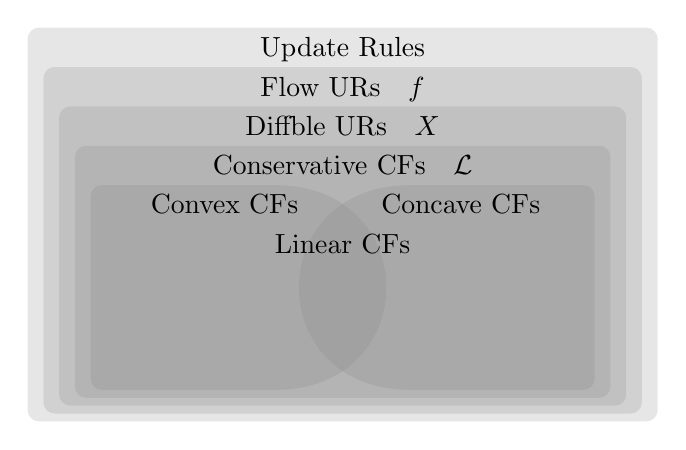
\begin{tikzpicture}
		\begin{scope}[fill=gray,fill opacity=0.2,rounded corners=4px]
			\fill (0,0) rectangle (8,5); % URs (Full Updates)
			\fill[] (0.2,0.1) rectangle (7.8,4.5); % Flow URs (Flows)
			\fill[] (0.4,0.2) rectangle (7.6,4.0); % Diffble URs (Vec Field)
			\fill[] (0.6,0.3) rectangle (7.4,3.5); % Conservative URs
			\fill (0.8,0.4) -- (0.8, 3.0) -- (3, 3.0)
			 	to[out=0,in=0,looseness=2] (3,0.4) --cycle; % CONVEX
			\fill (7.2,0.4) -- (7.2, 3.0) -- (5, 3.0)
			 	to[out=180,in=180,looseness=2] (5,0.4) --cycle; % CONCAVE
		\end{scope}
		\begin{scope}[anchor=north]
			\node at (4.0, 5.0) {Update Rules};
			\node at (4.0, 4.5) {Flow URs~~~$f$};
			\node at (4.0, 4.0) {Diffble URs~~~$X$};
			% \node at (4.0, 3.5) {Conservative CFs~~~$\mathcal L$};
			\node at (4.0, 3.5) {Conservative CFs~~~$\mathcal L$};
			\node at (2.5, 3.0) {Convex CFs};
			\node at (4.0, 2.5) {Linear CFs};
			\node at (5.5, 3.0) {Concave CFs};
		\end{scope}
	\end{tikzpicture}
	\caption{%
		A map of different kinds of commitment functions and their representations.}
	\end{figure}
	}

\begin{figure*}
% \centering
\begin{center}
~\hfill
\hspace{-3cm}
\begin{tikzpicture}
\begin{scope}[every node/.style={align=left,rounded corners=3,draw,thick,inner sep=5pt,anchor=center}]
	\node at (-3, 0) (fc) {%
		% Full-Confidence Update\\
		Full Update Rule \\
		% Update Rule \\
		$(\,\cdot\mid \cdot\,) : \Theta \times \Phi \to \Theta$\\
			\small\hfill\color{gray}(idempotent)\hfill};
	\node at (0, -3.4)(flow) {%
		% Complete Positive Flows\\
		% Commitment Flow\\
		% Flow Commitment Fn\\
		Flow Update Fn\\
		% Update Flow \\
		$
		% f
		\Lrn
		: [0,\infty] \times \Phi \times \Theta \to \Theta$\\
			\small\hfill\color{gray}(diffble, additive, limiting)\hfill};
	\node at (0, 3.4)(path) {
		% Smoooth Paths\\
		% Commitment Path\\
		% Path Commitment Fn\\
		% Path Update Fn \\
		Update Path \\
		$\gamma: [0,1] \times \Phi \times \Theta \to \Theta$\\
		\small\hfill\color{gray}(diffble, end-halting)\hfill};
	\node at (3.5, 0)(vfield) {%
		% Vector Fields \\
		Update Field \\
		$F : \Phi \to \mathfrak X(\Theta)$\\
		\small\hfill\color{gray}(complete, terminating)\hfill};
	\node at (8.5, 0) (loss) {%
		% Loss Repr \\
		% Incompatibility Measure \\
		% Loss Fn\\
		Plaus Function\\
		$\Bel: \Theta \times \Phi \to \mathbb R$};
	%%
	% \node at (-5, 3) (truth) {%
	% 	Truth Relation\\
	% 	${\models} : \Phi \times \Theta \to 2$
	% 	};
\end{scope}
	%% grad: loss to update fields
	\draw[arr] (loss) to node[above]{$\hat\nabla$} (vfield);

	%% commitment functions to update fields
	\draw[arr] (path) to[out=7,in=85]
		node[right=5pt,pos=0.7]{$\frac{\partial}{\partial s}$} (vfield);
	% \draw[arr] (flow) to[out=-7,in=-85]
	% 	node[right=3pt,pos=0.7]{$\frac{\partial}{\partial t}$} (vfield);
	\draw[arr] (flow) to[out=2,in=-90]
		node[left=3pt,pos=0.7]{$\frac{\partial}{\partial t}$} (vfield);

	%% update fields to commitment functions
	% \draw[arr] (vfield) to[out=-95,in=-2] node[above=0pt,pos=0.70]
	\draw[arr] (vfield) to[out=-85,in=5] node[right=1pt,pos=0.70]
		% {$\int \mathrm dt$}
		% {$\int dt$}
		% {$\int$}
		% {$\int (\,\cdot\,)\mathrm dt$}
		{$\int \,\cdot\,\mathrm dt$}
		% {$\int {-}\mathrm dt$}
		(flow);
	% \draw[arr1] (vfield) to[out=90,in=0] node[below right]{$\int \mathrm dt$} (path);
	% \draw (vfield) to[out=90,in=0] node[above]{$\int \mathrm dt$} (flow);
	
	%% full-confidence udpate rules from commitment functions
	\draw[arr] (path) to node[above, sloped]{$s=1$} (fc);
	\draw[arr] (flow) to node[below,sloped]{$t=\infty$}(fc);

	%% extra: dashed correspondence between commitment fns
	\draw[arr,-left to,dotted,gray] (path) edge[transform canvas={xshift=4pt}]
		node[right,pos=0.8,rotate=90]{$\scriptstyle-\log(1-s)$} (flow);
	\draw[arr,-left to,dotted,gray] (flow) edge
	 	node[left,pos=0.8,rotate=90]{$\scriptstyle1-e^{-t}$}(path);
	% \draw[arr,-left to] (path.south)++(0.1,0) to (flow.north)+(0.1,0);
	% \draw[arr,-left to] (flow.north) to (path.south);
	
	%% connections to truth
	% \draw[arr] (fc) to node[right]
	% 	% {$\models$}
	% 	{}
	% 	(truth);	
	% \draw[arr] (loss) to[out=130, in=0] 
	% 	node[above,pos=0.7]{local minima} (truth);
\end{tikzpicture}
\hspace{-3cm}\hfill~
\end{center}
\caption{Different representations of update functions, and the relationships they have with one another.
% Sections 3 and
}\label{fig:map}
\end{figure*}


% The final paragraphs of
% The last part of
% \cref{ex:classifier} illustrates an important aspect of confidence
Perhaps the most important application of confidence is in 
% to combine information from different sources with different degrees of trust.
% it allows us to update with with different degrees of trust.
% to treat different sources of information with different degrees of trust.
treating different sources of information with different degrees of trust.
As a result, one might imagine confidence to be relevant for sensor fusion:
    the problem of combining information
    from multiple different sensors (of varied reliability).
The standard approach to sensor fusion is called a Kalman
filter \parencite{kalman1960new,brown1997introduction}---%
and, indeed, comes with its own notion of confidence.


\begin{example}[1D Kalman Filter]
	\label{ex:kalman1d}
\def\estx{\hat{x}}
Suppose we are interested in modeling a
dynamical system whose state is a real number
$x \in \mathbb R$, and we recieve observations
% where $H$ is a matrix relating observations to state,
% $\mat z = H \mat x + \boldsymbol\xi \in \mathbb R^m$ where $H \in \mathbb R^{m \times n}$ is models a linear relation between states and observations,
% $z$ which we assume are a linear function of $x$,
$z$ which we assume is the value of $x$
% plus independent centered Gaussian noise of known variance $R$.
plus Gaussian noise.
% $\mat z = H \mat x + \boldsymbol\xi$,
% where $H \in \mathbb R^{m \times n}$, called the \emph{observation matrix} is a linear function, and $\boldsymbol\xi \sim \mathcal N(0, R)$ models random noise
% (which we assume is drawn independently from Gaussian with mean zero and covariance $R$).
% Suppose further that we re
In many engineering disciplines, the
 standard way to track this information is
% the Kalman filter \parencite{kalman1960new}.
the \citeauthor{kalman1960new} filter [\citeyear{kalman1960new}].
It prescribes belief state $(\estx, \sigma^2)$,
where $\estx \in \mathbb R$ is our current estimate of
$x$, and
% $P \in (-\infty,\infty]^{n\times n}$,
% $P \in \mathbb R^{n\times n}$
$\sigma^2$ is a variance
% (%
% Intuitively, this corresponds to a belief
% that
% $\mat x \sim \mathcal N(\estx, P)$.
% is normally distributed with mean $\estx$ and variance $P$.)
% (Intuitively, this amounts to a belief that
(effectively encoding the probabilistic belief
$x \sim \mathcal N(\estx, \sigma^2)$
% is normally distributed with mean $\estx$ and variance $\sigma^2$.
).
% (symbolically: $\mat x \sim \mathcal N(\estx, P)$).
%
% Suppose we now recieve an observation $\mat z$.
Suppose we now recieve an observation
% $z = x + \xi$, from a sensor whose noise $\xi\sim \mathcal N(0, r^2)$ has known variance $r^2$.
$z \sim \mathcal N(x, r^2)$ from a sensor of known variance $r^2$.
% For example, perhaps $\mat x = (x_1, x_2)$ is the location of an aircraft,
% and we have a sensor that
% % observes its first coordinate (plus noise), meaning that
% measures its first coordinate (plus noise $\xi$).
% This sensor's observation matrix
% $H$ then represents
% the map $(x_1, x_2) \mapsto x_1$, and we observe $\mat z = x_1 + \xi$.
How should we update our beliefs in response
% to $\mat z$
% to $z$
to this new information?

The right answer, which ranges from ignoring $z$ to replacing $\estx$ with it, depends on how much we trust the sensor.
The 1D Kalman filter measures confidence in the observation with a quantity $K$ called \emph{Kalman gain}, which is used to compute posterior beliefs
$(\estx', {\sigma^{2\prime}})$
% $(\estx', {\sigma'^{2}})$
 % as follows:
according to:
% we also have an objective quantity on which to base
% our assessment of the
\begin{align*}
	\estx' &= \estx + K (z - \estx)
         = (1-K) \estx + (K)\,z
		% \\
	;&
	% &\text{and}&&
	\sigma^{2\prime} &= (1 - K)^2 \sigma^2 + (K)^2 r^2.
    % = (I - KH) P,
    % \begin{pmatrix}
    %     \estx \\ P
    % \end{pmatrix}
    % &\gets
    % \begin{pmatrix}
    %     \estx + K (\mat z - H \estx) \\
    %      (I - K H)^{\sf T} P (I - K H) + K R K^{\sf T}
    % \end{pmatrix}
	% \\
	% &\text{where}~~ K = P H^{\sf T} (HPH^{\sf T} + R)^{-1}
\end{align*}
% we now argue that $K$
% We argue that it measures confidence in $\mat z$.
% can be veiewed as a measuring our confidence in the observation.
% acts as a ``blending factor''
% Because of the first update equation, $K$
% Often introduced as a ``blending factor'', $K$ is
% not so different from
% Observe the similarity between $K$ and 
% $\alpha$ in \cref{ex:prob-simple}:
Like other notions of confidence we have seen, $K$
interpolates (linearly) between our prior mean $\estx$ and the new observation $z$, and (``quadratically'') between our prior uncertainty $\sigma^2$ and the sensor variance $r^2$.
%
% Unlike the previous examples,
% Much more directly than in our previous examples,
Moreso than in previous examples,
we can also say something prescritive about how best to select
a degree of confidence.
This is made possible by two assumptions:
\commentout{
\begin{itemize}
    \item
    % We know the stochastic process by which observations $\mat z$ are generated,
    % including a number quantifying the reliability of observations (i.e., the variance $R$ of the noise $\boldsymbol\xi$ added to observations).
    % We know how observations $z$ are generated.
    We already have access to an objective quantification
    of the reliability of our observation $z$,
    through the variance $r^2$ of the noise $\xi$.
\item
    We would like to to select $K$ so as to minimize
    the uncertainty in our posterior beliefs, which happens to be
    the mean square error of our estimate $\estx$.
\end{itemize}
}
(1) we can objectively quantify the reliability of an observation (with the variance $r^2$),
and (2) the objective is to minimize uncertainty in our posterior beliefs (the mean squared error of $\estx$). 
Under these assumptions, the optimal Kalman gain is
% $K = P H^{\sf T} (HPH^{\sf T} + R)^{-1}$
% \begin{equation}\label{eq:opt-K}
$
    K_{\mathrm{opt}}
        = \ifrac{\sigma^2}{(\sigma^2 + r^2)}
    % K = P H^{\sf T} (HPH^{\sf T} + R)^{-1}
$
% \end{equation}
\parencite[p. 146]{brown1997introduction},
% and can be seen as the fraction of the variance of
% $K_{\mathrm{opt}}$ is the fraction of the total uncertainy
and so $K$ is typically chosen this way in practice
\parencite{kalmanfilter.net}.
% In principle any matrix is possible,but really
% the $(i,j)^{\text{th}}$ entry of $K$ .
% , in the sense that the posterior beliefs will minimize
% the expected mean square error
% Like before, this measure of confidence can be measured as lying between two extremes.
Plugging this value into the update equations, we find that this choice
makes $\estx'$ the average of our prior $\estx$ and new observation $z$,
weighted by their respective variances.

With this in mind, let's revisit what happens extreme values of confidence.
If $K = 0$, which
    % is prescribed by \eqref{eq:opt-K}
    is optimal
iff the noise $\xi$ has unbounded variance, then
    the update leaves our belief state unchanged.
In this case, there is intuitively so much noise in observations $z$ that
    we should not trust them at all.
%
At the other extreme, if no noise is added to observations ($r^2=0$),
then $K_{\mathrm{opt}} = 1$ and we end up with posterior $(z, 0)$
that fully trusts the new observation.
\end{example}


% The general case of Kalman filters for multidimensional state and observation, which we treat in \cref{ex:kalman-general}, is similar in spirit, but more involved.
	% and we must develop our mathematical apparatus somewhat before it fits cleanly into the picture we've laid out so far.
\cref{ex:kalman1d}
features
three distinct kinds of (un)certainty:
\begin{enumerate}
\item \textbf{Learner's Confidence:} a subjective trust in an observation
        which tells how seriously to take it in updating
        ($K$, in \cref{ex:kalman1d})
        ;
% $K$, a subjective confidence in the observation $z$,  which tells how seriously to take it in updating;
        % a feature of what one knows about where $\mat z$ comes from.
        % \label{item:kalman-gain}
    \label{item:learn-conf}

\item \textbf{Internal Confidence:}
        a way of quantifying the degree of uncertainty present in a belief state
        either overall
        or in a partircular proposition
        ($\sigma^2$ or the probability density
            $\phi \mapsto \mathcal N(\phi|\hat x, \sigma^2)$ in \cref{ex:kalman1d}, respectively);
    % $\sigma^2$, a subjective uncertainty in the current estimate $\hat x$, a feature of the current belief state;
	\label{item:internal-conf}

\item
    \textbf{Statistical Confidence:}
    an objective measure of the (un)reliablility of an observation,
    % based on historical information about related
    based on historical data and/or modeling assumptions about how
    observations arise
    (the noise level $r^2$, in \cref{ex:kalman1d})%
    .
    % $r^2$, an objective (un)reliablility of the observation $z$ (as measured by variance), a feature of the environment.
    % \label{item:measnoise}
    \label{item:stat-conf}
\end{enumerate}
The three can be closely related,
% but are quite different.
% but play very different roles.
    but are very different in nature.
Our focus is on confidence in sense \ref{item:learn-conf},
% Our examples have focused on
% quantities like \ref{item:kalman-gain},
% which we call confidences,
% and how they relate prior beliefs to posterior ones.
and how learning uses this kind of confidence
% to posterior beliefs.
to update beliefs.

We have tried to contrast learner's confidence (sense \ref{item:learn-conf})
with the more pervasive usage of the word ``confidence'' (sense \ref{item:internal-conf}),
such as likelihood, precision, or degree of belief.
% But they are related; such values may be thought of aggregated confidences
    % of past observations.
    % We explore the connections between them in the coming sections.
Other internal confidences
        include the probability $\Pr(\phi)$ in
        \cref{ex:prob-simple}, the degree
        of belief $\Bel(\phi)$ in \cref{ex:shafer},
        and the value of the loss function $\mathcal L(\theta,\phi)$
        used to train the classifier in \cref{ex:classifier}.
These two kinds of confidence are related:
    internal confidences may be thought of as aggregate
    reflections of learner's confidence in past observations.
    % ; such values may be thought of aggregated confidences
    % of past observations.
We explore these connections in more detail in the coming sections.

% We explore the connections between them in the coming sections.
% Prescriptions for how to select a numerical value for confidence
% are often functions of quantities such as \ref{item:measnoise}.

We would also like to distinguish our notion of 
	learner's confidence (sense \ref{item:learn-conf})
    from statistical confidences
    (sense \ref{item:stat-conf})
    such as the variance in readings
    of a sensor ($r^2$ in \ref{ex:kalman})
    or annotator agreement (from \cref{ex:classifier}).
% Under certain assumptions of independence, the two can
% Knowledge about
When readily available,
    % how reliable a sensor
    the statistical reliability of a source of information
    % should certainly inform how confident we in a given reading.
    should absolutely play a role in determining how seriously we take
    it in updating our beliefs---but it can be difficult to come by.
We may not always know the variances of our sensors, and that such a quantity is well-defined is a significant assumption on its own.  Statistical confidences typically require us to know that observations are drawn independently from a fixed distribution, while learners's confidence can be meaningful even without this assumption.

% We hope these examples have persuaded readers that confidence is ubiquitous and
% We hope that these examples have convinced the reader that confidence is ubiquitous, and given an intuitive sense of it.
% We hope that these examples have given the reader an intuitive sense of what confidence is, how ubiquitous it is, and why it is important.
% What's more, it also has a clean mathematical theory.
% But we have yet to say anything profound about it.
% We also find there to be a worthwhile underlying mathematical theory of confidence,
% which we develop in the coming sections.
% The rest of this paper is develops the theory of confidence,
%     by characterizing it axiomatically, and exploring what can be said of it in general.
% We develop
 % explores what can be said of it in general.


% We hope these examples have persuaded readers that confidence is ubiquitous and
% We hope that these examples have convinced the reader that confidence is ubiquitous, and given an intuitive sense of it.
We hope that these examples have given the reader an intuitive sense of what confidence is, how ubiquitously it arises, and why it is important.
What's more, it also has a clean mathematical theory.
% We now argue that it
% But we have yet to say anything profound about it.
% We also find there to be a worthwhile underlying mathematical theory of confidence,
% which we develop in the coming sections.
The rest of this paper develops the general theory of learner's confidence,
    characterizing it axiomatically (\cref{sec:updateformalism}), 
	
	% and exploring what can be said of it in general.
	
% We classify confidence functions, and develop three 
% We develop
 % explores what can be said of it in general.
% We will explore the 

\paragraph{Contributions.}
We have already motivated the notion of confidence and illustrated many of its most important properties by example.
In the remainder of the paper, we study confidence more formally. 
We develop a formal framework for talking about confidence.
% We describe cannonical representations of confidence.
We show that confidence can be measured in several equivalent ways, and classify the ways that 
In each stage, we make successively stronger assumptions (all of which apply to \cref{ex:prob-simple,ex:shafer,ex:classifier,ex:kalman1d}), to develop new representations of these learners, 
which are summarized in \cref{fig:map}.
The final representations we consider (vector fields and loss functions) also enable simultenous orderless updates, even in settings where it was not previously possible. 

% In \cref{sec:loss-repr}, we demonstrate that it is typically possible to get an even more compact representation of the updating process, by representing the vector field implicitly as gradients of some ``loss function''.


 % Once we have the formalism fully in place, we give further examples of how confidence works in exponential families, in particular showing how Kalman gain and inverse variance can be viewed as confidence as well.


 \commentout{
 This general idea can be cleaned up by appeal to differential geometry.
 Fix an input $\phi$.
 Assuming that the update paths are differentiable in the degree of confidence at any initial beleifs, the collection of updates with infinitessimal confidence forms a complete vector field $X_\phi$ over the space of beliefs, whose integral curves are paths in belief space, parameterized by confidence $\beta \in [0,\infty]$.
 % Of course, we may always convert this number back to $[0,1]$,
 We step through this more carefully in \cref{sec:field-repr}.

 %joe1*: NO!  This is not the place to bring up Reimannian metrics!
 Finally, if our belief space is endowed with a Riemannian metric, so that we may take gradients, partial update functions may be specified by a loss.}



\commentout{
	\subsection{Other Conceptions of Confidence.}

	\textbf{Probability.}
	% Probability is a numerical scale that ranges from untenable (0) to undeniable (1).
	% No number on this scale is truly neutral.
	% One of the biggest shortcomings of probability is its inability to represent a truly neutral attitude towards a proposition.
	Some people do use ``confidence'' to mean the same thing as probability. When they say they have low confidence in $\phi$, they mean that they think $\phi$ is unlikely.

	One of the biggest shortcomings of probability is its inability to represent a truly neutral attitude towards a proposition.
	%  probability of $\frac12$ .
	% This shortcoming has perhaps been the primary selling point of many alternatives to probabiltiy, such as Dempster-Shafer Belief functions.
	A value of $\frac12$ may be equally far from zero as it is from one, but is by no means a neutral assessment in all cases: hearing that your favored candidate has a 50\% chance of winning is big news if a win was previously thought to be inevitable.
	For this reason, telling someone the odds are 50/50 is quite different from saying you have no idea.
	% By contrast, zero confidence represents a truly neutral stance; a statement with zero confidence has no effect.
	By contrast, zero confidence represents something truly neutral:
		a statement made with zero confidence does not stake out a claim, and
		a statement recieved with zero confidence does not affect the recipient's beliefs.
	Nevertheless, in some contexts, we will see that confidences correspond to to probabilities.

	\textit{Opacity.} To use a graphical metaphor, think of certainty as black or white.
	Probability describes shades of gray, while confidence describes opacity.
	If we are painting with black and start with a white canvas, there is a precise correspondence between the opacity and the resulting shade of gray.

	\textbf{Upper and Lower Probabilities.}
	Upper and lower probabilities can describe a neutral attitude towards a proposition, but they are not really a specification of trust, but rather a direct specification of a belief state.
	It isn't immediately clear how to use these representations of uncertainty to update, and they're a little too complex to function effectively as the primitive measure of trust that we're after.


	\textbf{Shafer's Weight of Evidence.}
	Shafer's ``weight of evidence'' is precisely the same concept we have in mind.
	Our analysis precsely reduces to his, in the setting where belief states are Belief functions (which generalize probabilities, but not, say, neural network weights), and observations are events.
	% This paper can be a generalization of Shafer's ``weight of evidence'' to a broader class of settings, where one might have very different belief states and observations.
	Thus, this paper can be viewed as generalizing this concept to a broader class of settings, without requiring that one adopt Shafer's conception of a belief state or an observation.


	\textbf{Variance and Entropy.}
	The inverse of variance, sometimes known as precision,
		is also commonly used to measure confidence.
	If a sensor is unreliable and can give a range of answers, the variance of the estimate is a very common way of quantifying this reliablility.
	If measurements have zero variance, in some sense one has absolute confidence ($\top$) in the sensor. If measurements have infinite variance, then in some sense one has no confidence in the sensor, since individual samples convey no information about the true value of the quantity measured.
	As with probability, inverse variance will coincide with confidence in some settings; we will see how in \cref{sec:variance}.

	Entropy, like variance, is a standard way of measuring uncertainty, and in some settings, confidence coincides with entropy (see \cref{sec:entropy}).
	The assumption underlying both approaches is that there's some ``true'' value of the variable, and that the randomness is epsistemic (due to sensor errors) rather than aleotoric (inherrent in the quantity being measured).

	\textbf{Confidence Intervals and Error Bars.}
	Another notion of the word ``confidence'' comes from the term ``confidence interval''.
	This concept arises in settings involving a probability distribution $\Pr(X)$ over a metric space $X$, typically $X = \mathbb R$.
	A 95\% confidence interval is the (largest) ball containing 95\% of the probability, and its size is a geometric measurement of how .
	This intuition behind this reading of the word confidence is the same as
}






%%%%%%%%%%%%%%%%%%%% UPDATE FORMALISM %%%%%%%%%%%%%%%%%%
Our formalism consists of three parts: 
	a domain $\confdom$ of confidence values,
	a space $\Theta$ of belief states, and
	a language $\Phi$ of possible observations. 
For instance:
% For example, the learning settings in our examples are
\begin{itemize}[nosep,itemsep=1pt,left=0.5em]
    \item In \cref{ex:prob-simple}, $\Theta$ is the set of probability
    measures on some measurable space $(\Omega, \mathcal F)$,
    $\Phi$ is the $\sigma$-algebra $\cal F$, and the confidence domain
    is $[0,1]$.
    % Then
    % the context is
    % \[
    %     \Big(\Delta \Omega,~
    %         \mathcal F,~
    %          (A,\alpha,\mu) \mapsto (1-\alpha)\mu + \alpha (\mu|A)
    %     \Big).
    % \]
    \item In \cref{ex:shafer}, $\Theta$ is the set of belief functions
    over a finite set $W$, $\Phi = 2^W$ is the set of subsets of $W$,
    % and there are variants for both $[0,1]$ or $[0,\infty]$.
    and confidence is a degree of support $\alpha \in [0,1]$
    or a weight of evidence $w \in [0,\infty]$.
    \item In \cref{ex:classifier}, 
	% $\Theta = \overline{\mathbb R}^d$ is
	$\Theta \subseteq \bar{\mathbb R}^d$ is
    the space of network parameters, $\Phi = X \times Y$ is the space of 
    input-lablel pairs, and the confidence domain is the
	 	extended natural numbers $\{0, 1,\ldots, \infty\}$ under addition.
    % In \cref{sec:smooth-completion} we will extend this example to to continuous confidences in $[0,\infty]$.
	%
	\item In \cref{ex:kalman1d}, $\Theta = \Phi = \mathbb R$, and $\confdom = [0,1]$ is the domain of $K$. 
\end{itemize}
Together, we call the triple $(\Theta, \Phi, \confdom)$ a \emph{learning setting}.
	% and we will be interested in studying the learners for a given setting. 
% Before we put them all together 
% (in \cref{sec:learning-setting-funcs})
A \emph{learner} in the
 % learning
setting $(\Theta, \Phi, \confdom)$
is a function
\commentout{\unskip\footnote{%
	% we can just as easily handle randomized updates;
	It should be straightforward to extend our theory
	so as to handle randomized updates as well;
	the point is that
	% the update can be prescribed by an algorithm.
	the belief state, observation, and confidence must together contain
	enough information to describe the updating process.
}}
% \[
$
	\Lrn : \Phi \times \confdom \times \Theta \to \Theta
$
% \]
% that must satisfy certain axioms.
% First, we want to ignore untrusted information, i.e.,
% used to incorporate new observations into the belief state.
that describes the belief update process.
Explicitly: from a prior belief $\theta$, and a statement $\phi$
	with some degree of confidence $\chi$,
	% it
	a learner 
	produces a posterior belief state
	$\Lrn(\phi,\chi,\theta) \in \Theta$.
We use superscripts and subscripts to
% partially specify
fix some arguments
of $\Lrn$ and view it as a function of the others, so that
$\Lrn(\phi,\chi,\theta)$
can equivalently be written as
$
	\Lrn_\phi(\chi,\theta) = \Lrn^\chi_\phi(\theta)
	= \Lrn^\chi(\phi,\theta) = \Lrn_{(\theta,\phi)}(\chi)
		 % = \Lrn^\chi_\theta(\phi)
		 .
$
% We will also impose axioms to ensure 
% Most of this section is devoted to 
The rest of this section develops axioms and auxiliary concepts that ensure that these functions capture the the update procsss. 

% Before we get there, 
% to describe the learning settings in the introduction, 
% But we do so in pieces ,
We do so in three stages, starting with two fragments of the theory that isolate some critical mathematical properties of confidence. 
The first an abstract theory of confidence domains $\confdom$ themselves
	(\cref{ssec:confdom});
 	the second is a theory of \emph{commitment functions}, which introduce $\Theta$ and describe the update process (\cref{ssec:comm-func}). 
Finally, we bring in the observations $\Phi$ (\cref{ssec:full-learn}).


% \subsection{A Formal Model}
% \subsection{Abstract Confidence Functions and Domains}
% \paragraph{Abstract Confidence Domains.}
\subsection{Abstract Confidence Domains}
	\label{ssec:confdom}
A \emph{confidence domain} $(D, \le, \bot, \top, \oplus, \mathfrak g)$
% is an ordered set $D$
is a set $D$
of confidence values 
equipped with a preorder $\le$,
a 
% is an ordered set $D$ of confidence values, 
% $D$ has a 
% special least element
least element
$\bot$ (``no confidence''), a greatest element
$\top$ (``full confidence''),
and an operation $\oplus$ that combines two independent degrees of confidence into a single one. 
% of confidence with a single degree of confidence.
We often abreviate a confidence domain as $D = \confdom$,
leaving $\le$ and $\oplus$ implicit.
%
% The intuition that $\oplus$ represents \emph{independent} combination
% 	suggests that it should be commutative and associative.
Because $\oplus$ represents \emph{independent} combination,
	we require that it be commutative and associative. 
% We want to ignore independent untrusted information,
% and complete trust combined with another independent confidence
% remains complete trust.
% Furthermore, combining some degree of confidence $\chi$ with an independent no-confidence should have no effect on $\chi$, and combining with an independent.
We want to ignore independent information we have no confidence in, and, if already fully confident, remain so the face of new independent information. 
Formally, this amounts to requiring, for all $\chi,\chi',\chi'' \in D$:
\begin{itemize}[parsep=0pt,itemsep=1pt,label={}]
% \begin{CDaxioms}[parsep=0pt,itemsep=1pt]
\item $(\chi \oplus \chi') \oplus \chi'' = \chi \oplus (\chi' \oplus \chi'')$
    \hfill (associativity)$\mathrlap{,}$
		\hspace{1cm}\;\;
\item $\chi \oplus \chi' = \chi' \oplus \chi$
    \hfill(commutativity)$\mathrlap{,}$
		\hspace{1cm}\;\;
\item $\bot \oplus \chi = \chi$
    \hfill (that $\bot$ is neutral)$\mathrlap{,}$
		\hspace{1cm}\;\;
\item $\top \oplus \chi = \top$\;
    \hfill (and that $\top$ is absorbing)$\mathrlap{.}$
		\hspace{1cm}\;\;
% \end{CDaxioms}
\end{itemize}
% We typically also assume that $D$ comes equipped with a topology or a differentiable structure.
Finally, $D$ comes with geometric information $\mathfrak g$, which may 
	optionally include a topology, a differentiable structure.
	% , or a Riemannian metric. 
		% \unskip\footnote{see \cref{appendix:geometry} for a }
		% (At this point, the reader only needs to know is that these are increasingly specific notions of geometry, but we provide a short review in \cref{appendix:geometry} for completeness.)
% Two confidence domains are particularly common.
% We now introduce two particularly important confidence domains
% We now formally introduce two
Our work will focus on two
 	particularly important confidence domains 
		describing describe a continuum of confidence,
		both of which appear in our examples.
% Many of our examples use
The first is the \emph{fractional domain} $[0,1]$,
whose elements $s \in [0,1]$ represent 
	the ``proportion of the way towards complete trust''.
If you go proportion $s$ towards fully trusting something,
then $s'$ of the remaining way, then overall
you have gone
% $\alpha \oplus \alpha'
% := \alpha + \alpha' (1-\alpha) = 
% \alpha + \alpha' - \alpha \cdot \alpha'$
$s \oplus s'
:= s + s' (1-s) = 
s + s' - s \cdot s'$
    of the way to complete trust.
The other confidence domain of particular interest
 	is the \emph{additive domain} $[0,\infty]$, which is
	ideal for analogies of time and weight.
    % is roughly the amount of time you spend updating your beliefs.
We will later see that the two are isomorphic,
	and have a particularly rich theory.
	
\begin{prop}
	The fractional domain $[0,1]$ the additive domain $[0,\infty]$ are isomorphic.
	Furthermore, the space of isomorphisms between them 
		% (and hence the space of automorphisms of each)
		is
	 	% naturally with $\beta \in (0,\infty)$, according to
		% itself isomorphic to the set of real numbers.
		in natural bijection with $(0,\infty)$.
	Specifically, for each $\beta \in (0,\infty)$, there is
		an isomorphism $\varphi_\beta : [0,1] \to [0,\infty]$ given by
	\[
		% [0,1] \ni s \xmapsto - \log(1-s) 
		% \begin{array}{ccc}
		% 	[0,1] \ni s  &\mapsto& -\frac1\beta \log(1-s) \\
		% 		1- \exp(-\beta t) &\mapsfrom& t \in [0,\infty]
		% \end{array}
		[0,1] \ni s = 1-e^{-\beta t} = \varphi_\beta^{-1}(t)
			% ~\leftrightarrows~
			\qquad\text{and}\qquad
			 \varphi_\beta(s) = -\frac1\beta \log(1-s) = t \in [0,\infty]
			 .
	\]
\end{prop}

\commentout{
This way of combining numbers in $[0,1]$ is a little more
complicated, and it's not as apparent that it has nice properties
like associativity (although it does). However,
% all of the nic
\cref{ax:fractionality} has essentially the same implications as 
\cref{ax:additivity},
and there are certainly cases where intuition for this scale
is stronger.
}

%%% it's false that a total order imposes a unique confidence domain.
%%% so too is it false that 1d implies uniqueness. Think \max, or a graded sequence of updates. 
% \begin{prop}
% 	% Up to isomorphism $[0,\infty]$ is the
% 	There is a unique confidence domain 
% \end{prop}
%
% \paragraph{Commitment Functions.} 
% Let $\Theta$ be a set, possibly equipped with a topology and/or differentiable structure. A function $f: \confdom \times \Theta \to \Theta$ is
% a $\confdom$-\emph{commitment function} for $\Theta$ 
% if it satisfies


	% ;
    % these confidence domains have a particularly rich theory, which we develop
    % in \cref{sec:smooth}.

	% \subsection{Learning Settings and Update Functions}
	% We now introduce the critical missing components: beliefs and observations.
	% \paragraph{Learning Settings and Learners.}
	\subsection{Belief States and Commitment Functions}
	% \subsection{Modeling Belief: State and Commitment Functions}
		\label{ssec:comm-func}
	% \paragraph{Learning Functions.}
	% \paragraph{Learning Functions.}
		\label{sec:learning-setting-funcs}
	%
	% For instance:
	% % For example, the learning settings in our examples are
	% \begin{itemize}[nosep,itemsep=1pt,left=0.5em]
	%     \item In \cref{ex:prob-simple}, $\Theta$ is the set of probability
	%     measures on some measurable space $(\Omega, \mathcal F)$,
	%     $\Phi$ is the $\sigma$-algebra $\cal F$, and the confidence domain
	%     is $[0,1]$.
	%     % Then
	%     % the context is
	%     % \[
	%     %     \Big(\Delta \Omega,~
	%     %         \mathcal F,~
	%     %          (A,\alpha,\mu) \mapsto (1-\alpha)\mu + \alpha (\mu|A)
	%     %     \Big).
	%     % \]
	%     \item In \cref{ex:shafer}, $\Theta$ is the set of belief functions
	%     over a finite set $W$, $\Phi = 2^W$ is the set of subsets of $W$,
	%     % and there are variants for both $[0,1]$ or $[0,\infty]$.
	%     and confidence is a degree of support $\alpha \in [0,1]$
	%     or a weight of evidence $w \in [0,\infty]$.
	%     \item In \cref{ex:classifier}, 
	% 	% $\Theta = \overline{\mathbb R}^d$ is
	% 	$\Theta \subseteq \bar{\mathbb R}^d$ is
	%     the space of network parameters, $\Phi = X \times Y$ is the space of 
	%     input-lablel pairs, and the confidence domain is the
	% 	 	extended natural numbers $\{0, 1,\ldots, \infty\}$ under addition.
	%     In \cref{sec:smooth-completion} we will extend this example to
	%      to continuous confidences in $[0,\infty]$.
	% \end{itemize}
	%
	% A \emph{learning setting} $(\Theta, \Phi, \confdom, \Lrn)$
	%     is an updating context together with a function
	% An \emph{update function}
We now reintroduce the space $\Theta$ of beliefs, 
	% which come with a topology or a differentiable structure,
	for the purpose of characterizing how confidence effects belief updates. 
In this section, we describe the essential properties 
	of of confidence in terms of functions
	$\Lrn_\phi : \confdom \times \Theta \to \Theta$. 
Many of the most important aspects of confidence can be characterized purely in terms of such functions, keeping $\phi$ entirely abstract.
We call a function of this type a \emph{commitment function}, if it is obeys certain axioms.
% A function $f : \confdom \times \Theta \to \Theta$,
% 	which one should think of as $\Lrn_\phi$ for some fixed $\phi$ whose nature is irrelevant, satisfying the axioms of this section 
% 	is called a \emph{commitment function}. 
% However, for 
% We consider properties
%
%
% In order to capture our intuition of producing posterior beliefs,
% $\Lrn$ must also satisfy certain axioms.
% First, we want to ignore 
% 	% untrusted information.
% 	information in which we have no confidence.
First, having no confidence ($\bot$) in an observation
	means we should ignore it. 

\begin{LrnAxioms}
		% [nosep,itemsep=1pt]
    \item
		% [LRN1]
        % [(zero)]
		$
		\forall \phi,\theta.\quad
		% \forall \theta.\quad
		\Lrn(\phi,\bot, \theta) = \theta
		% f^\bot(\theta) = \theta
		$
        % \hfill (ignore untrusted info)
        \label{ax:zero}
\end{LrnAxioms}

Second, we intend for $\Lrn$ only to be used to incorporate information to the extent that it is novel,
i.e., information that is not already accounted for in our prior beliefs.
% \TODO[INDEPENDENCE DISCUSSION]
%
Thus, we would like a sequence of two (independent)
observations in the same observation $\phi$ to
be equivalent to a single observation of $\phi$ 
with their combined degree of confidence.
% ; see
 % \cref{ssec:indep-shafer} for further discussion of this matter.

\begin{LrnAxioms}
	\item 
	% $\forall \phi, \theta,\chi,\chi'.\quad$
	$\forall \phi, \chi,\chi'.\quad$
	% $\forall \theta,\chi,\chi'.\quad$
	% $\forall \chi,\chi'.\quad$
	%%% version with scripts and no $\theta$
	% $\Lrn_\phi^\chi \circ \Lrn_\phi^{\chi'} = \Lrn_\phi^{\chi\oplus\chi'}$
	%%% version with parens
	% $\Lrn(\phi, \chi, \Lrn(\phi, \chi', \theta)) =  \Lrn(\phi, \chi\oplus\chi',\theta)$.
	%%% version with \phi subscript
    $\Lrn_\phi(\chi, \Lrn_\phi(\chi', \theta)) =  \Lrn_\phi( \chi\oplus\chi',\theta)$.
	%%% version with f
	% $f^\chi \circ f^{\chi'} = f^{\chi\oplus\chi'}$
        \label{ax:combinativity}
\end{LrnAxioms}

% It is worth pausing here
The reader is encouraged
 to verify that \cref{ex:prob-simple,ex:kalman1d} satisfy \cref{ax:combinativity} for the domain $[0,1]$.
For a specific confidence domain, 
% we will soon see that
\cref{ax:combinativity} can be quite a strong assumption. 
However, if we are free to chose the confidence domain, \cref{ax:combinativity} imposes no restrictions at all (see \cref{prop:free-additivity} in the appendix).
% This says nothing about how to combine confidences in different
% observations, nor about the effect of $\phi'$ between the two updates.
{\color{gray}%
Keep in mind that \cref{ax:combinativity} applies only for two
observations of the same statement $\phi$.
}%
% A reader with a background in algebra might observe that \cref{ax:zero} and \ref{ax:combinativity} are together equivalent to requiring that $\Lrn_\phi$ be a monoid action of $(\confdom, \oplus, \bot)$ on $\Theta$. What about the remaining structure of the confidence domain: the top element ($\top$) and the order ($\le$)? What should it mean for $\Lrn$ to respect these parts of a confidence domain?
In the language of algebra, \cref{ax:zero} and \ref{ax:combinativity} together require $\Lrn_\phi$ to be an \emph{action} of the monoid $(\confdom, \oplus, \bot)$ on $\Theta$.
% Yet the monoid $(\confdom, \oplus,\bot)$ is not a 
Beyond the data of this monoid, a confidence domain $D$ also has 
	an order ($\le$),
	a geometry,
	and an absorbing top element ($\top$). 
% What about the remaining structure of the confidence domain: the top element ($\top$) and the order ($\le$)? What should it mean for $\Lrn$ to respect these parts of a confidence domain?
% The question of what it means for $\Lrn$ to preserve this structure leads us to additional axioms characterizing full-confidence udpates and, respectively. 
What should it mean for $\Lrn$ to preserve this additional structure? 
% One answer is \cref{ax:ineq-witness}, which we discuss in the appendix,
% but it is perhaps more intuitive
% But there is also another answer.
% The answer is what makes learner's confidence so unique. 



% Next, for geometry. 
\textbf{Geometry.}
Learner's confidence is meant to interpolate between 
	ignoring new information and defering to it entirely,
	% thus, we would like the path of intermediate confidences to 
	and the most natural (and useful) interpolations are continuous and smooth.
	
\begin{LrnAxioms}
	\item
	If $\confdom$ and $\Theta$ are both topoplogical spaces, then 
	for all $\theta$ and $\phi$, 
	the map
	$
	\Lrn_{(\theta,\phi)} = 
	\chi \mapsto 
	\Lrn(\theta,\chi,\phi)
	$
	is continuous.
	If $\confdom$ and $\Theta$ are both manifolds, then 
	$\Lrn_{(\theta,\phi)}$ is 
	% a differentiable map.
	differentiable.
		\label{ax:cont-and-smooth}
\end{LrnAxioms}
Ideally, the update would be continuous in our initial
beliefs as well: similar priors typically result
in similar posterior beliefs.
% This would allow us to strengthen \cref{ax:cont} to something simpler:
This suggests a simple strengthening of \cref{ax:cont-and-smooth}:
% \begin{LrnAxioms}[nosep]
% 	\item
% 	[L{\the\numexpr\value{LrnAxiomsi}\relax}${^\prime}$]
% 	$\Lrn_\phi :\confdom \times \Theta \to \Theta$ 
% 	is continuous
% 		(resp. differentiable)
% 	for all $\phi \in \Phi$.
% 	\label{ax:cont-strong}
% \end{LrnAxioms}
that
$\Lrn_\phi :\confdom \times \Theta \to \Theta$ 
be continuous (resp. differentiable)
Unfortunately,
% \cref{ax:cont-strong} 
that is too strong to handle our examples at full confidence.
In the probabilistic case, for instance:

% Axiom \cref{ax:cont-strong} says more---it says that the posterior 
% belief is also continuous in the prior beliefs, 
% which also seems appropriate. But this assumption has significant bite.
% \commentout{%
% actually, this shows a problem with defining 
%
% \begin{example}
% 	Again let $W$ be a finite set, and choose disjoint non-empty subsets
% 	$A, B \subset W$ with $A \cap B = \emptyset$.
% 	Let $p\ne q$ be two distinct distributions over $W$ supported
% 	on $A$, and $d$ be one suppoerted on $B$. Now, consider 
% 	% and consider a sequence $(\mu_i)_{i \in \mathbb N}$ of positive probability 
% 	% distributions over $W$ whose limit 
% 	% is the point mass $\delta_w$ on a particular world $w \in W$.
% 	% $\mu^*$ has support $A \subsetneq W$ (i.e., $\mu^*(A)=1$).
% 	the two sequences of probability distributions
% 	\[
% 		\Big(p_n= (1-e^{-n}) d + (e^{-n}) p \Big)_{n \in \mathbb N}
% 		,
% 		\qquad
% 		\Big(q_n = (1-e^{-n}) d + (e^{-n}) q \Big)_{n \in \mathbb N},
% 	\]
% 	both of which have limit $d$. But every $p_n | A = p$ while every $q_n |A = q$, so
% 	now \cref{ax:cont-strong} implies that 	
% \end{example}%
\begin{prop}
	\label{prop:no-continuous-condition-ext}
	%joe3: I don’t understand what you mean by this.
	% There is no continuous extension of conditioning to a function
	% $F$ satisfying \cref{ax:cont-strong}.
	There is no extension of conditioning that satisfies \cref{ax:cont-strong}.
	%
	% That is, if $(W, \mathcal F)$ is a measurable space $\Phi = \mathcal F$,
	% and $\Theta$ consists of all probability measures on $(W, \mathcal F)$, then
	% there is no continous function $F : $
	% In particular, 
	That is,
	% if $\Theta = \Delta W$ and $\phi\subset W$ is an event,
	for $\phi\subsetneq W$,
	there is no continuous function
	$F_\phi : \Delta W \times [0,1] \to \Delta W$
	such that $F_\phi(\mu, 1) = \mu|\phi$ when $\mu(\phi) > 0$. 
	% nor even one whose restriction to  $ [0,\epsilon) \times \Phi \times \Theta \to \Theta$
	% is continuous, for $\epsilon > 0$.
\end{prop}
% This is a consequence of the fact that there's no 
% continuous extension of conditioning that handles
% observations of events that have probability zero.
%
Intuitively, though, this is just an edge case; we can still get continuity
if we never observe an event we believe has probability zero. 
% So, rather than insist that updates are always continuous in our priors, 
% Rather than insist that updates always be continuous in our priors,  we simply take note of a set of priors for which 
Rather than insisting on this stronger axiom or giving up on it entirely, we can get something in between 
% with a proposition instead of an axiom
% with a proposition in place of the axiom: 
% learning a particular $\phi$ is continuous. 
with the following definition.

\begin{linked}{defn}{maximal-continuous-theta}
	% For all $\phi \in \Phi$,
	% there is a maximal open set $\Theta_\phi \subseteq \Theta$ such that
	% the restriction 
	Given $\phi \in \Phi$, let $\Theta_\phi \subseteq \Theta$ be the maximal set 
	open set for which the restriction
	$
	% F_{\phi} |_{\Theta_\phi} : 
	\Lrn_{\phi} |_{\Theta_\phi} : 
		% [0,1) \times \Theta_\phi \to \Theta
		[\bot,\!\top) \times \Theta_\phi \to \Theta
	$		
	of 
	% $F_\phi$
	$\Lrn_\phi$
	to $\Theta_\phi$ is continuous. 	
\end{linked}
In each of our examples, $\Theta_\phi$ consists of those
of belief states that do not flatly contradict $\phi$.
In \cref{ex:prob-simple}, 
for instance, \cref{prop:no-continuous-condition-ext,prop:maximal-continuous-theta}
imply that $\Theta_\phi = \{ \mu \in \Delta W : \mu(\phi) > 0\}$
is the set of distributions $\mu$ on which conditioning on $\phi$ is well-defined.
% \footnote{
% For those familiar with the basic anatomy of an ML system: 
% in \cref{ex:classifier}, if $\phi=(x,y)$, then $\Theta_{\phi}$ is the set of weights for which the gradients $\nabla_{\theta}\ell(f_\theta(x), y)$ of the loss function $\ell$ are finite.
In \cref{ex:classifier}, if $\phi=(x,y)$, then $\Theta_{\phi}$ is the parameter space in which the gradients $\nabla_{\theta}\ell(f_\theta(x), y)$ of the loss function $\ell$ are finite.
 % }
 
 % From a learner's perspective, 
 \textbf{Order.}
 For a learner,
 	% what characterizes an update with less confidence is that 
 	% the confidence ordering is characterized by being able to get the same effect with another update later on.
 	the characteristic property of $\chi \le \chi'$ is that
 	learning with confidence $\chi$ is more conservative than learning with $\chi'$,
 	in the following sense:
 	% After learning $\phi$ with confidence $\chi$, one can obtain 
 	one can get the effect of learning $\phi$ with higher confidence by first learning with lower confidence, and then making a second update with some residual degree of confidence.


 \begin{LrnAxioms}
 	\item
 	% When $\chi \le \chi'$, there exists some $\chi'' \in \confdom$ such that
 	% $\Lrn_\phi^{\chi} \circ $
 	$\forall \phi, \theta,\chi,\chi'.\quad$
 	$\chi \le \chi'$ 
         % if and only if
         $\quad\iff\quad$
         % there exists $\chi'' \le \chi'$ such that
         $\exists \chi'' \le \chi'.~~$
 		%%% version with f
 		% $f^{\chi''} \circ f^\chi = f^{\chi'}$.
 		%%% version with sub and superscripts
 		% $\Lrn_\phi{\chi''} \circ \Lrn_\phi^\chi = \Lrn_\phi^{\chi'}$.
 		%%% version with subscripts and \theta	
 		$\Lrn_\phi^{\chi''} \circ \Lrn_\phi^\chi (\theta) = \Lrn_\phi^{\chi'}(\theta)$.
 		%%% version with subscripts and no \theta
 		% $\Lrn_\phi^{\chi''} \circ \Lrn_\phi^\chi = \Lrn_\phi^{\chi'}$.
 		%%% version with parens
 		% $\Lrn(\phi, \chi'', \Lrn(\phi, \chi, \theta))  = \Lrn(\phi, \chi', \theta)$.
 		% \!\!\!\!
         \label{ax:ineq-witness}
 		\label{ax:seq-for-more}
 	\item[\cref*{ax:seq-for-more}$^{<}$]
 	% When $\chi \le \chi'$, there exists some $\chi'' \in \confdom$ such that
 	% $\Lrn_\phi^{\chi} \circ $
 	$\forall \phi, \theta,\chi,\chi'.\quad$
 	$\chi < \chi'$ 
         $\quad\iff\quad$
         $\exists \chi'' < \chi'.~~$
 		$\Lrn_\phi^{\chi''} \circ \Lrn_\phi^\chi (\theta) = \Lrn_\phi^{\chi'}(\theta)$.
        \label{ax:ineq-witness-strict}
 		\label{ax:seq-for-more-strict}
 \end{LrnAxioms}
 Observe that, in the presence of \cref{ax:combinativity}, the right hand side of \cref{ax:ineq-witness} is tautology when $\chi' = \top$ or if $\chi = \bot$; thus our axioms would have implied $\bot \le \chi \le \top$ for all $\chi$ even had we not assumed this. 
 There is a sense in which \cref{ax:ineq-witness} can viewed as a limited form of subtraction for confidences, although the result of that subtraction may be nondeterministic and depend on $\theta$ and $\phi$. 
 
 % The point of the monotonicity condition \cref{ax:seq-for-more} is to rule out cases such as the one depicted below, in which 
 In some sense, the effect of \cref{ax:seq-for-more} is to rule out cases 
 in which ``stopping and resuming'' an update 
 % in a completely different path 
 results in completely different beliefs than we would have obtained with a single update. 
 \cref{ax:seq-for-more} also ensures
 	that a high confidence update can be decomposed into
 	several updates of lower confidence. 
 \begin{center}
 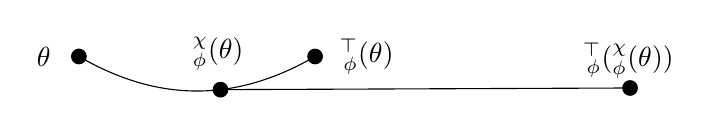
\begin{tikzpicture}
     \coordinate[label=left:$\theta~~$] (A) at (0,0);
     \coordinate[label=right:%
 		% $~\theta\phi$% 
 		$~~\Lrn_\phi^{\!\top}(\theta)$%
 		] (C) at (3,0);
     \coordinate[label=above:%
 		% $F_\phi^{.6}(\theta)\mid\phi$%
 		$\Lrn_\phi^{\!\top}(\Lrn_\phi^{\chi}(\theta))$%
 		] (C') at (7,-0.4);
     \draw (A) to[bend right] 
 		node[outer sep=0,pos=0.6,label=above:%
 			% $F_\phi^{.6}(\theta)$%
 			$\!\Lrn_\phi^{\chi}(\theta)$%
 			](B){} (C);
     \fill 
         (A) circle (0.1)
         (B) circle (0.1)
         (C) circle (0.1)
         (C') circle (0.1);
     \draw (B.center) to (C');
 \end{tikzpicture}
 \end{center}
 For the domain $[0,\infty]$ (and hence, in $[0,1]$, which is isomorphic to it), \cref{ax:ineq-witness} and its strict analogue L4{$^{<}$}
 are direct consequences of \cref{ax:combinativity}. 



% \paragraph{Full-confidence updates}
\textbf{Full-confidence updates.}
% {\color{red}
Historically, most of the literature on belief updates is about 
	idempotent updates, which in our framework, correspond to full-confidence updates.
{\color{red}Full updates are quite extreme.
An agent that updates by conditioning, for instance,
% is permanently commited to believing everything it ever learns with perfect certainty,
permanently commits to believing everything it ever learns,
and gains nothing from making the same observation twice.
 % (\cref{ax:idemp})
% Humans don't work this way. The effectiveness of flash cards as a learning tool demonstrates this clearly: if we were using an update rule, two cycles through a deck of flash cards would be no different from one.
Clearly humans are not like this; revisiting information
 	improves our learning \parencite{ausubel1965effect}.
Similarly, artificial neural networks are trained with
 	many incremental updates, and benefit from seeing 
	the training data many times.
% Indeed, this is one biggest differences between modern machine learning techniques and  older rule-based ones: modern algorithms update parameters little-by-little, rather than fully incorporating input information.
% Once an agent that uses conditioning incorporates $A$, it is forever committed to believing $A$, and as a side effect, there is no point to making
We would like an account that allows for for less extreme belief alterations,
in which information is only partially incorporated.
This is the role of intermediate degrees of confidence.
}

Finally, we turn the top element of the confidence domain.
Our axioms already have some implications for it. 
% Our axioms so far already tell us 
% Because $\Lrn$ reflects the order structure of $\confdom$ (\cref{ax:ineq-witness})
% 	and $\top$ is the largest element, it follows that 
% 	for all $\chi$, there is some $\chi'$ such that 
% 	$\Lrn_\phi^{\chi'}$
Because $\Lrn$ preserves monoidal structure (\cref{ax:combinativity})
	and $\top$ is absorbing, it follows that 
	$\smash{\Lrn^\top_\phi} : \Theta \to \Theta$ is a projection,
	i.e., $\smash{\Lrn^{\top}_\phi \circ \Lrn^\top_\phi = \Lrn^\top_\phi}$. 
% Furthermore, 
% $\Lrn^{\top}_\phi \circ \Lrn^\top_\phi = \Lrn^\top_\phi$
% This allows us to define
This suggests that we could use $\Lrn$ to define the 
 	belief states in which ``$\phi$ is true'' to be
	image of this projection (i.e., the set of fixed points of $\smash{\Lrn^{\top}_\phi}$);
% ($\im \Lrn^\top_\phi$)
% as the 
after all, it is easily shown that learnining $\phi$ with any degree of confidence (i.e., applying $\Lrn_\phi^\chi$) has no effect on these states. 
This illustrates a general point: if the function $\Lrn$ captures the
	belief updating process, we can use it to understand the relationship between $\Phi$ and $\Theta$ at an abstract level.
	In \cref{ex:classifier}, for instance, 
		although the network weights $\Theta$ are an uninterpreted subset of some high dimensional space, 
		the training process $\Lrn$ 
		arguably imbues them with meaning by defining
			a connection between them and the training examples.
					
% However, 
% to some readers, this may seem backwards:
%
% However, u
However, to some readers, using $\Lrn$ to define truth may seem backwards.
In a given learning setting, we may already have a sense of
which belief states $\theta$ correspond to full belief in $\phi$---in \cref{ex:prob-simple}, for instance, 
% belief states are probability measures, and so already ascribe (a degree of) truth to events $\phi$. 
	they are the measures that give $\phi$ probability 1.
In such cases, we may want additional axioms ensuring that 
	any relationships between $\Theta$ and $\Phi$ implicit in $\Lrn$
	are compatible with the ones we already have. 
% and want to require that $\Lrn\!^\top$ projects to the \emph{correct} subspace.
Our axioms so far have been conditions on the separate functions
	$
	% \{
	\Lrn_\phi : \confdom \times \Theta \to \Theta
	% \}_{\phi \in \Phi}
	$, 
	but we have not required that $\Lrn_\phi$ be intrinsically related $\phi$. 
 	% we want to impose another axiom ensuring that this definition of
	% truth lines up with one
	%  % we already had in mind.
	%  already present.
	% analogous to \cref{ax:zero}
To address this, we will need to assume some additional structure.
% although it will turn out that the mathematical study of the objects at hand is equivalent if we simply take the approach above (\cref{theorem:}). 


\hidewithbox{
	% \bigskip
	%%%%%%%%%%%%%%%%%%%%%%%%%%
	% \paragraph{[MOVEME]}
	Finally, we impose a mild regularity condition
	that can be thought of as
	% a special case arising in 
	a limit \cref{ax:seq-for-more}
	when confidences $\chi_1$ and $\chi_2$ become infinitessimally close;
	% for infinitessimal values of confidence (specifically $\chi_1$),
	% which we can make sense of because of \cref{ax:diffble}. 
	% which we can make sense of via differentiability (\cref{ax:diffble}). 
	we make this precise via differentiability (\cref{ax:diffble}). 
	% The next axiom states
	% This is a relatively minor condition

	\begin{LrnAxioms}
		\item \label{ax:nopause}
		% \commentout{% oli's initial version, with derivative
			If
			% $\frac{\partial}{\partial\chi} F(\theta,\chi,\phi) \!=\! 0$
			$\frac{\partial}{\partial\chi} F^\chi_\phi(\theta) = 0$
			and $\chi' > \chi$,
			then 
			% $F(\theta, \chi', \phi) \!=\! \theta$.	 
			$F^{\chi'}_\phi(\theta) = \theta$.
		% If $\chi' > \chi$ and $F(\chi, )$
	\end{LrnAxioms}

	%joe3: CF6 also says that there are no saddle points. Why is that reasonable?
	%oli3: since confidence is 1-dimensional, the notion of a saddle point doesn't apply. We're just talking about a differentiable path in belief space, and we're saying that it does not halt.

	Intuitively, \cref{ax:nopause} amounts to requiring that updates
	do not ``temporarily pause'' for intermediate values of confidence,
	and then resume for higher values of confidence.
	The culmination of these axioms results in our first definition of an
	update function that takes confidence into account.


	% For this reason, we give them a special name
	% Together, these axioms allow us to define an update rule, by:

	\begin{defn}
		A
		\emph{path update function} is a 
		function $F: \Phi \times [0,1] \times \Theta \to \Theta$ 
		satisfying
		\cref{ax:zero,ax:idemp,ax:cont,ax:seq-for-more,ax:diffble,ax:nopause}.
		% is an \emph{update function}.
		% is a \emph{path commitment function}.
		% is a \emph{path update function}.
	\end{defn}


	Path update functions capture many of the most important aspects of 
	uncertain observation, but they are complex and difficult to work with.
	In the next section, we will
	 % see how  
	see a different perspective on the same axioms,
	which will ultimately allow us to 
	put path update functions in a standard form, 
	which can be extended to handle combinations of inputs weighted
	by relative confidence.
	% Path update functions capture some important aspects of uncertain
	% updating%
	% ---but a number $\chi \in [0,1]$ is not the only useful
	% way to quantify confidence.
	% For the full picture of of how these concepts are related, we will
	% need to look at confidence from several more angles.
}%

\commentout{%
A function $f : \confdom \times \Theta \to \Theta$,
	which one should think of as $\Lrn_\phi$ for some fixed $\phi$ whose nature is irrelevant, satisfying the axioms of this section 
	\[
	\Big(f^\bot = \mathrm{id}_{\Theta}, 
	\quad
	f^\chi \circ f^{\chi'} = f^{\chi\oplus\chi'},
	\quad
	\forall\theta. \chi\le\chi'\text{ iff }\exists\chi''. f^{\chi\oplus\chi''}(\theta) = f^{\chi'}(\theta),
	\quad
	\chi\mapsto f^\chi(\theta) \text{ continuous}
	\Big)
	\]
	is called a \emph{commitment function}. 
}


% \paragraph{Belief and Learning.}
% \subsection{Modeling Observations: Learning, Belief, and Structural Symmetry}
\subsection{Modeling Observations: 
	Degree of Belief, and Structural Symmetry}
	\label{ssec:full-learn}
Recall that a \emph{learning setting} is a triple $(\Theta, \Phi, \confdom)$
consisting of
    a space $\Theta$ of beliefs,
    a language $\Phi$ of observations,
    and a confidence domain $\confdom$.

\textbf{Belief.~~}
In a learning setting $(\Theta, \Phi, \confdom)$,
a \emph{believer} is a function $\Bel : \Theta \times \Phi \to \confdom$,
and can be thought of as annotating each state $\theta$ with a function $\Bel_\theta : \Phi \to \confdom$ that gives a degree of belief to each observation. 
% This form of confidence 
Thus the ouput of a believer is an \emph{internal} confidence---like a probability or a precision---not a learner's confidence.
Our primary reason for defining $\Bel$ is that 
	we would like $\Lrn$ to be monotonic with respect to $\Bel$.
    That is, learning $\phi$ with more confidence
    should lead to more belief in $\phi$.

\begin{LrnBelAxioms}
	\item 
	$\forall \phi,\theta,\chi,\chi'.\quad$
	$\chi \ge \chi'
	% \quad\implies\quad
	~~\implies~~
	\Bel(\phi, \Lrn(\phi,\chi,\theta)) \ge \Bel(\phi, \Lrn(\phi, \chi', \theta))
	% \Bel_\phi \circ \Lrn_\phi(\chi,\theta) \ge \Bel_\phi \circ \Lrn_\phi(\chi', \theta)
	$.
		\label{ax:monotone}
\end{LrnBelAxioms}

We cannot ask for strict monotonicity, however:
if we already fully believe $\phi$ (i.e., $\Bel(\phi,\theta) = \top$),
% we cannot attain a higher degree of belief by learning $\phi$.
there is no way to attain a higher degree of belief, we cannot attain a higher degree of belief by learning $\phi$.
% Next, if we already believe $
% Instead, if we fully believe $\phi$, learning $\phi$ should
Instead, if we fully believe $\phi$, learning $\phi$ should
	have no effect.
Perhaps even more importantly, 
 	if we learn something with full confidence, then we ought to fully believe it.
\begin{LrnBelAxioms}
\item If $\Bel(\phi,\theta) = \top$, then
    $\Lrn(\phi,\chi,\theta) = \theta$. 
    \label{ax:truth-is-enough}
% \end{LrnBelAxioms}
% 
% % Finally, perhaps a
% The converse of \cref{ax:truth-is-enough}
% % $\Bel$ also allows us to be more precise about the effect of
% an intuitive characterization of full-confidence updates:
% if we learn something with full confidence, then we fully believe it.
% 
% \begin{LrnBelAxioms}
    \item $\Bel(\phi, \Lrn(\phi,\top,\theta)) = \top$.
        \label{ax:effectiveness}
\end{LrnBelAxioms}

While
\cref{ax:effectiveness} is certainly desirable,
		it may not always hold in cases of interest.
	% setting up the model so that this is true may not be worthwhile.
	In \cref{ex:classifier}, for instance,
		it is natural to set $\Bel(\theta,(x,y)) = f_\theta(y|x)$,
	and there may be a local maximum $\theta$ of the parameterization
		$\theta \mapsto \Bel(\theta,(x,y))$.
	In this case, there is no continuous monotonic path from $\theta$ to a global maximum $\theta^*$ for which $f_{\theta^*}(y|x) = 1$,
	i.e., no way to simultaneously satisfy 
	\cref{ax:monotone,ax:effectiveness,ax:cont-and-smooth}.

% In the abstract setting where $\Theta$ and $\Phi$ have no a priori, 
% however, axioms \cref{ax:monotone,ax:truth-is-enough,ax:effectiveness}
% have no bite.
% \begin{linked}{prop}{synthetic-bel}
% 	For every learner $\Lrn$, there exists a 
% 	believer $\Bel$ such that the pair $(\Lrn, \Bel)$ satisfy 
% 	\cref{ax:monotone,ax:truth-is-enough,ax:effectiveness}
% \end{linked}

% Thus, a no-confidence update simply discares the new observation.
% At the opposite extreme, we call $F^1_\phi$ a \emph{full update}. 
% The appropriate way to deal with full confidence depends
% At the opposite extreme, the appropriate way to deal with full confidence
% The appropriate way to deal with full confidence, on the other hand,
% depends on the relationship between $\Theta$ and $\Phi$.

% but it still characterized by an important property.
% but it can still be characterized at this level of generality.

% \textbf{High Confidence Updates.}


% Not only 
% 
% \begin{LrnAxioms}
% 	\item[\ref*{ax:idemp}']
% 	% Full-confidence updates are idempotent.
% 	% For all $\phi \in \Phi$, the update $F_\phi$ is idempotent.
%     % That is, for all $\phi \in \Phi$,  $F^1_\phi \circ F^1_\phi = F^1_\phi$.
%     % That is, for all $\phi \in \Phi$ and $\theta \in \Theta$,  $F^1_\phi \circ F^1_\phi = F^1_\phi$.
%     % (i.e., $F^1_\phi \circ F^1_\phi = F_\phi$).
% 	$F^\chi_\phi \circ F^\chi_\phi = F^\chi_\phi$ iff $\chi \in \{0,1\}$
% 		or $\phi$ is trivial (in the sense that $F^\chi_\phi(\theta) = \theta$ for all $\phi,\chi,\theta$).
% 	\label{ax:idemp-strong}
% \end{LrnAxioms}
% 




% Now, we're not quite in the same position as Shafer.
% Shafer was prescribing a concrete representation of $\Theta$ (a belief function) and a concrete update rule $F$ (Dempster's rule of combination), and so he needed to defend these choices.
% We only need to defend something much more modest: we only need to defend the assumption that, if $\Theta$ and $\Phi$ properly model the relevant aspects of the scenario at hand, then there exists \emph{some} function $F$ which performs updates appropriately.


% \subsection{
% 	% Continuity and
%  	% The Path of Middling Confidence
% 	% Paths of Intermediate Confidence
% 	Intermediate Confidence Values
% 	}



% $\theta$ such that
% the loss $\mathcal L(\theta, \phi) < \infty$ that the training algorithm minimizes is finite.

\textbf{Symmetry.}
We would also like update rules to preserve any joint symmetries between the belief space $\Theta$ and the observation language $\Phi$.
For instance, in \cref{ex:prob-simple}, we would like to require that updates are not sensitive to irrelevant relabelings of points.
% Concretely, let $\mathrm{Aut}(X, \Phi)$ be the set of automorphisms $\sigma : X \to X$, together with an action on assertions, so that $\sigma\phi \in \Phi$ is the appropriately relabeled assertion equivalent to $\phi$ after the relabeling.
Concretely, assume we have some set $\mathrm{Aut}(\Theta, \Phi)$ of 
	structural symmetries
	(in the form of automorphisms $\sigma : (\Theta \sqcup \Phi) \to (\Theta \sqcup \Phi)$)
	% $\sigma : \Theta \to \Theta$ 
	that have an action both on belief states ($\sigma(\theta) \in \Theta$) and 
		on observations ($\sigma(\phi) \in \Phi$).
	% (say, rotations of the simplex of distributions), that also have an associated action on assertions, so that $\sigma\phi \in \Phi$ is the corresponding relabeling of $\phi$ under $\sigma$.  
		The symmetry condition can now be captured by:
\begin{LrnAxioms}
	\item
	% For all 
	$\forall \theta,\phi,\chi,~~
	 \sigma
	% : X \to X
	% \in \mathrm{Aut}(X, \Phi)$, we have
	\in \mathrm{Aut}(\Theta, \Phi)
	% $, we have
	.\quad$
% \\ \indent\hspace{2em}
% $F^\beta_A(\sigma_\#(\Pr)) = \sigma_\#\Big(F^\beta_{\{\sigma(a) : a \in A \}}(\Pr)\Big)$,
% $F^\beta_\phi (\sigma_\#(\Pr)) = \sigma_\#\Big(F^\beta_{\sigma\phi}(\Pr)\Big)$,
% $F^\beta_{\sigma\phi} (\sigma(\theta)) = \sigma \Big( F^\beta_{\phi}(\Pr)\Big)$.
% $\Lrn_{(\sigma(\theta),\sigma(\phi))} = \sigma \circ \Lrn_{(\theta,\phi)}$.
% $\Lrn_{(\sigma\theta,\sigma\phi)} = \sigma \circ \Lrn_{(\theta,\phi)}$.
$\Lrn(\sigma(\phi), \chi , \sigma(\theta)) = \sigma (\Lrn(\theta,\chi, \phi))$.
	% \hfill \textbf{(symmetry)}
	 \label{ax:symmetry}
\end{LrnAxioms}

%%%%%%%%%%%%%%%%%%%%%%%%% COMBINATIVE + VFields %%%%%%%%%%%%%%%%%%%%%%%%%%%%%%%%%

\section{Commitment on Confidence Continua}
% For convenience of measurement, and so that we may better study confidence as a \emph{smooth} interpolation between ignoring and fully incorporation, we shall focus primarily on cases where confidence can be measured as a real number.
In this section, we focus precisely on the special case in which the confidence domain is a continuum of real numbers. 
There are two particularly important confidence domains in this setting are the fractional domain $[0,1]$ and the additive domain $[0,\infty]$.


%joe3: bad story. Just say that you want additivity.
%oli3: bringing up text about additivity, and reduing stress on scale.
% Recall that the number of training iterations $n$ in \cref{ex:classifier}
% and Shafer's weight of evidence $w$ in \cref{ex:shafer}
% are measurements of confidence that do not lie in $[0,1]$, but
%  rather in $[0,\infty]$.
Most quantities 
used in science and everyday life
can be measured additively:
if one starts with seven minutes/meters/votes/dollars,
and then gains six
 % additional (distinct) ones, 
more,
one has thirteen altogether.
% We would like a measure of confidence that also works this way.
% What is measure of confidence that works this way?
% We would like to be able to measure confidence in the same way.
% Wanting to measure confidence the same way gives us the domain $[0,\infty]$. 
To measure confidence in the same way, we must use the domain $[0,\infty]$. 
With this confidence domain, \cref{ax:combinativity} means $\Lrn$ is \emph{additive},
making it amenable to analogies of weight (e.g., the weight of evidence $w$ in \cref{ex:shafer})
and time (e.g., the number of training iterations $n$ in \cref{ex:classifier}).
Indeed, a learner is addive iff it can be implemented so that confidence really does coincide with time: imagine a machine with state space $\Theta$, controlled by buttons labeled by $\Phi$, that, while $\phi$ is pressed, evolves from initial state $\theta_0$ according to $\theta(t) = \Lrn(\phi, t, \theta)$. 
Observe that this scenario is coherent if and only if $\Lrn$ is additive; if \cref{ax:combinativity} did not hold, there would exist $t_1,t_2$ such that the machine's state after pressing $\phi$ for $t_1$ seconds followed by $t_2$ additional seconds, would be different from the configuration after holding down $\phi$ for $t_1+t_2$ seconds.

% This temporal analogy may not always be appropriate 
Temporal analogies may not always be appropriate
% For instance, 
(as they may clash with other, truer conceptions of ``time''),
yet they have such intuitive force that 
% yet the intuition 
a function
$f: [a,b] \times \Theta \to \Theta$  
	% (with $a\le 0 < b$)
	(with $0 \in [a,b] \subseteq \mathbb R$)
satisfying \cref{ax:zero,ax:cont-and-smooth,ax:combinativity}
is known generically as a \emph{flow} \parencite{lee2013smooth}.
\commentout{
    Beyond \cref{ax:diffble,ax:additivity},
    $F$ need only handle full-confidence
    appropriately (i.e., satisfy \cref{ax:idemp,ax:cont})
    in order to satisfy all of our axioms thus far.}%
% Due to \cref{prop:additivity-implications} and the fact that 
%     \cref{ax:diffble} is stronger than \cref{ax:cont}, 
% the flow axioms 
% (\cref{ax:additivity},\cref{ax:diffble})
% imply all of our axioms so far
% (\cref{ax:zero,ax:idemp,ax:cont,ax:diffble,ax:seq-for-more,ax:nopause,ax:additivity}).
Recall that \cref{ax:combinativity} implies \cref{ax:seq-for-more} 
	for this domain.
	% the additive case. 
Thus, the only non-standard requirement is that $\Lrn_{(\theta,\phi)}$ has a well-defined limit at $\infty \notin\mathbb R$. 
%
% To some, the domain $[0,\infty]$ and 
The assumptions that confidence lies in $[0,\infty]$ and combines
additively are collectively quite strong, and one might understandably
worry that it could limit the applicability of our formalism.
Fortunately, this is not the case.
While 
additivity (\cref{ax:combinativity} for $[0,\infty]$) 
does pin down how confidence
can be measured, it has no effect on what confidence can express.

\begin{linked}{theorem}{add-reparam}
	If $\Lrn 
	% : \Phi \times \confdom \times \Theta \to \Theta
	$ 
	% satisfies \cref{ax:zero,ax:combinativity,ax:cont-and-smooth,??}
	satisfies \cref{ax:zero,ax:cont-and-smooth,ax:seq-for-more,??}
	(but possibly not \cref{ax:combinativity})
	then there exist
	% a
	% flow update function
	$^+\!\Lrn$
	and a continuous function
	$g : \Phi \times [\bot,\!\top] \times \Theta \to [0,\infty]$
	% and a function $g$
	such that
	% for all $\theta,\phi,$ and $\chi$,
	% for all $\theta\in\Theta,\phi\in\Phi,$ and $\chi\in[\bot,\!\top]$,
	% \[
	\[
		\forall \theta,\phi,\chi.\qquad
		\Lrn( \phi,
			\chi,
		 \theta )
		 =
		{^+}\!\Lrn(\phi,~
		% \beta,
		g(\phi,\chi,\theta),~
		 \theta)
		 \qquad\text{and}\qquad
		{^+}\!\Bel(\phi,\theta) = g(\phi, \Bel(\phi,\theta),\theta)
		.
	\]
	% Furthermore, $^+\!F$ and $g$ are unique up to a multiplicative factor,
	% and so
	% there is a unique choice of $(^+\!F,g)$
	% such that $^+\!F$ and $F$ handle smallconfidences in the same way,
	% i.e., $\frac{\partial g}{\partial \chi} = 1$.
	Furthermore,
	% $^+\!F$ and $g$ are unique up to a multiplicative factor
	% the pair
	 $(^+\!F, g)$ is unique up to a multiplicative factor
	% in the additve representation of confidence.
	% in the additive representation of confidence (i.e., the output of $g$).
	in the output of $g$.
	% (that may depend on $\phi$ and somewhat on $\theta$).
	% (that can depend on $\phi$, and partially on $\theta$).
	% (that can depend on $\phi$ and $\theta$).
		% \footnote{ can depend on $\phi$, 
		% and $[\theta] \in \Theta / (\theta_1 \sim \theta_2 \text {if})$}.
	\end{linked}
\begin{coro}
There is a unique choice of $(^+\!F, \beta)$
% such that $^+\!F$ and $F$ handle small confidences the same way,
% i.e., $\frac{\partial g}{\partial \chi}|_{\chi=0} = 1$.
such that $^+\!F$ and $F$ have the same effect on observations
made with sufficiently low confidence, 
i.e., $\frac{\partial \beta}{\partial \chi}\big|_{\chi=\bot} = 1$.
% that behaves like $F$ for low confience updates
% (and is also additive: \cref{ax:additivity}).
% Furthermore, there exists a function
\end{coro}

Thus, updates performed with $F$ are equivalent
to updates performed with ${^+}\!F$, except that
the degree of confidence needs to be translated appropriately (via $\beta$).
We call $^+\!F$ the \emph{additive form of $F$},
and $\beta(\phi, \chi, \theta)$ the additive form of 
confidence $\chi$. 
% This quantity might, unfortuna tely, depend on $\theta$, and $\chi$.
% Unless $F$ is strangely parameterized,
% If confidence to $F$ is meaningful independent of $\theta$ and $\phi$,
% then so too should 
% knowing 
Ideally,
the translation $g$ to an additive scale should not depend
on our current beleifs $\theta$ or observation $\phi$.

% It would be  dependence of $g$ on $\theta$ and $\phi$ is
% somewhat unsavory, and would $F$ 

\commentout{%%% uniformity
\begin{defn}
We call an update function $F$ \emph{uniform} if 
the additive form
$g(\phi,\chi,\theta)$
of its confidence depends only on $\chi$
(and not on $\theta$ or $\phi$). 
\end{defn}

\cref{ax:additivity} implies uniformity, as then $^+\!F = F$ 
and
$g(\phi,\chi,\theta) = \chi$.
}%%% end uniformity


% \subsection{Vector Field Representations}
% \subsection{Update Fields}
% \subsection{Order of Obsevation and the Vector Fields of Commitment Functions}
\subsection{The Vector Fields of Commitment Functions, and Orderless Combination}
\label{sec:vecrep}

% Suppose we learn $\phi_1$, and then $\phi_2$ (for simplicity, say with the same confidence $\chi$). 
Suppose we learn $\phi_1$ (with confidence $\chi_1$), and then $\phi_2$ (with confidence $\chi_2$). 
% Is this the same as learning $\phi_2$ and then $\phi_1$? 
Is this the same as learning them in the opposite order?
This is true of belief functions 
% ((\cref{ex:shafer}, perhaps a reason to find belief functions attractive)
(\cref{ex:shafer}) and of conditioning, so we call them \emph{commutative}%
---but, in general, 
observing inputs in different orders yields different results.
Humans tend to have a recency bias: more recent observations have a stronger influence on beliefs.
\Cref{ex:prob-simple,ex:kalman1d} have this property as well.
% But often pieces of information at once, we would like to update using that combined information.
% Nevertheless, even if prioritizing recent information is appropriate, 
% Still, 
But, the order matters for our update, what should we do if we recieve two pieces of information simultaneously?
% it would seem problematic to prioritize one piece of information over another if they are recieved simultenously. 
	% if one were two pieces of information together, 
	% we would like to update using that combined information.
% It turns out that there is already a natural way to do this, even
It turns out that we already have the tools to do this in a natural way, even
% the update function 
if $\phi_1$ and $\phi_2$ do not commute.  
% if the order in which one observes $\phi_1$ and $\phi_2$ matters.
% if $\phi_1$ and $\phi_2$ do not commute.  

% We now investigate 
We now turn to an equivalent representation of 
flow
% or fractional 
update functions, which, among
other things, will ultimately
yield a natural way of
% orderlessly combine observations, and 
orderlessly learning $\phi_1$ and $\phi_2$ together, and weighted by relative
confidence. 
%
At a technical level, we show how to
extend an arbitrary update function $F$, that handles inputs $\Phi$,
% to a set $\ext\Phi \supseteq \Phi$ with some algebraic operations.
to handle a more expressive set of inputs $\ext\Phi \supseteq \Phi$
closed under new operations of
orderless combination ($\oplus$), and rescaling by relative confidence ($\cdot$).

% In \cref{ax:diffble}, we assumed that $\Theta$ has a differentiable structure; thus, 
Since $\Theta$ carries a differentiable structure,
it makes sense to talk about its tangent space
%joe3: please add parens!
%oli3: parens are non-standard in this context. See Lee 2013,
%   which is the standard reference on manifolds, or even the
%   wikipedia page.
$T\Theta$,
which consists of pairs $(\theta, \mat v)$ where
$\theta \in \Theta$, and $\mat v$,
% is intuitively an infinitessial direction rooted at $\theta$.
intuitively, is a direction that one can travel in $\Theta$ beginning at $\theta$
% tangent to $\Theta$
% rooted at $\theta$
\parencite[\S3]{lee2013smooth}.
% structure; for ease of presentation, suppose that it is an $n$-dimensional manifold \parencite{lee2013smooth}.
% For a smooth manifold $M$ (such as the space $\Delta \X$ of distributions over $\X$),
% and a point $p \in M$, we follow convention by writing $T_p M$ for the tangent space to $M$ at point $p$ \parencite{lee2013smooth}, and % $TM := \sqcup_{p \in M} (p, T_p M)$
% $TM := \sum_{p \in M} T_p M$ for the full tangent bundle over $M$.
%
% A vector field over $M$ is a smooth map $\mat v : M \to T M$ assigning a tangent vector $\mat v(p) \in T_p M$, to every point $p \in M
%
A \emph{vector field} $X \in \mathfrak X\Theta$ is a
% smooth
differentiable
map $X : \Theta \to T \Theta$
assigning to each point  $\theta \in \Theta$
a vector $X(\theta) = (\theta, \mat v) \in T\Theta$
tangent to $\theta$.
\commentout{
	The set of all vector fields over $\Theta$ is denoted $\mathfrak X(\Theta)$
	 % and is closed under linear combination
	 and forms a vector space.
	\parencite[\S8]{lee2013smooth}
	\unskip.
	}%
%
% There is a close relationship between additive confidence and such vector fields.
% There is a close relationship between additive confidence and such vector fields.
% A vector field is called \emph{complete} if it generates a global flow.
% , or equivalently, a smooth section of the projection map $\pi : T M \to M$, where $\pi((p, v)) = p$.
Additivity (\cref{ax:combinativity})
% (and indeed even \cref{ax:seq-for-more})
implies that the behavior of flow update functions is determined by the
way it handles updates of small confidence.
So, in a sense, the only thing we need to know about
a flow update function is how it handles infinitessimal confidences,
which is to say, its derivative at zero confidence---which can be
viewed as a vector field.
More precisely,
% given a commitment function 
a commitment function
% $F$, and observation $\phi$,
$\Lrn_\phi$
% we can define the \emph{vector field of $\phi$} by
has a \emph{vector field representation} given by
% differential of $F_\phi$
% intuitively represents an update with infinitessimal confidence,
% and is a vector field
\begin{equation}
	% F'_\phi
	% F'_\phi
	% \mathrm{d}\Lrn_\phi
	\Lrn'_\phi
	:=
	\theta \mapsto
	% \frac{\partial}{\partial \chi} F_{\theta}^{\chi} \Big|_{\chi=0}
	% \frac{\partial}{\partial \chi} \Lrn_{(\theta,\phi)}(\chi) \Big|_{\chi=0}
	\frac{\partial}{\partial \chi} \Lrn(\theta, \chi, \phi) \Big|_{\chi=\bot}
	\qquad\in 
	\mathfrak X \Theta
	.
	\label{eq:f-field}
\end{equation}
Moreover, we can recover $\Lrn_\phi$ via the integral curves of $\Lrn'_\phi$.
% In other words, if we knew only the vector field $F'_\phi$,
% we could
% because $F_\phi$ is the unique function satsifying \eqref{eq:f-field}.

\begin{fact}[{\citeauthor[Thm 9.12]{lee2013smooth}}]
	If $X \in \mathfrak X(\Theta)$,
	there is at most one
	 % function
	$f : [0,\infty) \times \Theta \to \Theta$
	such that for all $\theta \in \Theta$ and $a,b\ge 0$,
	\[
	f(a, f(b, \theta)) = f(a+b,\theta)
		~~\text{and}~~
	\frac{\partial}{\partial \chi}
	 	f(\chi,\theta)
		% \underset{\chi=0}|
		\Big|_{\chi{=}0}
		\!\!= X(\theta)
		.
	\]
	\label{fact:unique-integral-curves}
\end{fact}
\begin{coro}
	% Suppose $X_\phi \in \mathfrak X(\Theta)$ be a vector field.
	% Let $F$ be a flow-update rule.
	% Suppose $X_\phi \in \mathfrak X(\Theta)$ be a vector field.
	% Then there is at most one flow-update function satisfying \eqref{eq:f-field}.
	% Fix the vector field $X := F'_{\phi}$.
	% $F$ is the only flow-update rule satisfying \eqref{eq:f-field}.
	%%%v1
	% Let $F$ be a flow update function, and fix the vector field $F'_{\phi}$.
	% Then $F_\phi$ is the only flow update function satisfying \eqref{eq:f-field}.
	%%%v2
	If $F_{\phi_1}$ and $F_{\phi_2}: \Theta \times[0,1] \to \Theta$ are distinct,
	then so are $F'_{\phi_1}$ and $F'_{\phi_2}
	 % \in \mathfrak X(\Theta)
	$.
	%%%v3
	% If $F$ is the uni
	\label{fact:unique-flow-for-vfield}
\end{coro}

% Therefore, \cref{theorem:add-reparam}
Thus, every 
% flow update function $F$
flow update function $F$
 can be equivalently represented
by its differential $F'$, a collection of vector fields.
% \begin{prop}
% 	% Let $F$ be a flow-update rule.
% 	% Then, there is a bijective correspondence between
% 	There is a biective correspondence between
% 	flow-update rules
% 	% $F : \Phi \times[0,\infty] \times \Theta \to \Theta$.
% 	and
% 	$\Phi$-indexed families of vector fields $X : \Phi \to \mathfrak X(\Theta)$.
% % Every update rule $F : \Phi \times \mathbb R \to (\Theta  \to \Theta)$
% % satisfying \cref{ax:zero,ax:additivity,ax:diffble} corresponds to a unique
% % $\Phi$-indexed collection of vector fields
% %     $F' : \Phi \times \Theta \to T\Theta$
% \[
% 	X()
% \]
% \end{prop}
% \begin{coro}\label{thm:vecrep}
%     There is a natural bijection between
%     % update rules $F : \Phi \times \mathbb R \to \Delta \X \to \Delta \X$
%     update rules $F : \Phi \times \mathbb R \to (\Theta  \to \Theta)$
%         satisfying \cref{ax:zero,ax:additivity,ax:diffble},
%     and $\Phi$-indexed collections of complete vector fields
%         % $\{ F'_\phi : \Delta X \to T \Delta X \}_{\phi \in \Phi}$%
%         % $\{ F'_\phi : \Theta \to T \Theta \}_{\phi \in \Phi}$%
%         $ F' :  \Phi \times \Theta \to T \Theta$%
%         % $F' : \Phi \to \Delta\X \to T\Delta \X$%
%     .
% \end{coro}
% In the language of
%
% Not all vector fields can be integrated to get an update function
%
% \begin{coro}\label{thm:vecrep}
% There is a bijective correspondence between udpate rules satisfying \cref{ax:zero,ax:additivity,ax:diffble} and $\Phi$-indexed collections of \textbf{complete} vector fields.
% \end{coro}
% We call $F'$ the \emph{vector field representation} of an update function $F$.
% This vector field representation of an update function
It may seem counter-intuitive that $F'_\phi$,
which no longer explicitly mentions confidence at all,
can capture confidence.
 % In a sense, it does so by specifying
But it does---in a sense, by specifying
everything about the update \emph{except} for the degree of confidence.
This vector field representation is useful for two reasons:
at a practical level, it gives us a natural extension of $\Phi$
that allows us deal with ``mixtures'' of observations and commonly arise.
At a deeper level, it will enable us to describe and classify
the flow update functions on $\Theta$.
% Having separated the confidence from the mechanics of the update,
% this vector field representation allows us to describe and
% classify update functions on $\Theta$

% \subsection{Orderless Combination of Observations}
% \textbf{Orderless Combination of Observations.}
One important feature of vector fields is that they
% form a vector space, and so
can be linearly combined to form new vector fields.
% Therefore, flow update functions,
Since in the presence of a flow update function,
observations correspond to vector fields,
observations also inherrit this linear structure.
%
There are two aspects of linearity: scalar multiplication, and addition.
% The first way of combining
From scalar mutliplication, we get a way of rescaling
inputs
% $\phi$
by a ``relative confidence'' $k
 % \in [0,\infty)
$.
% \begin{prop}
	% Suppose $F$ is a flow udpate rule.
% For $\phi \in \Phi$, we can extend $F$
Concretely, given $\phi \in \Phi$ and $k \in [0,\infty)$,
 % given $k$ and $\phi$,
define a new observation
% $k\cdot\phi \in \ext\Phi$
$k\cdot\phi$
% and extend $F$ to handle it by:
and extend $F$ to
a function $\ext F$ that handles it by:
\[
	F^{\chi}_{k\cdot\phi}(\theta) := F^{k\chi}_{\phi}(\theta)
	,\quad\text{or equivalently,}\quad
	F'_{k\cdot \phi} := k F'_{\phi}
	.
\]
% \end{prop}
Note that if $k > 0$, the rescaled input
$k\cdot \phi$ behaves the same way that $\phi$
does for extreme values of confidence,
since $k 0 = 0$ and $k\infty = \infty$.

% In this way, the set $\Phi$ inherits
% the additivity of the update rule in the form of scalar multiplication.
% It turns out more is possible: updates inherit the entire vector space structure.


% The second way of combining propositions is to ``observe them concurrently''.
% The second way we
% Making use of vector field addition, we can also
From vector field addition, we get a natural way to combine observations.
Up to now, we have only been able to combine observations provided they are
both of the same input $\phi$ (e.g., via \cref{ax:additivity}).
The vector field representation allows us to do this for distinct inputs.
% This can be quite powerful.
% In particular, given commitment functions $F, G : \mathbb R \to \Theta$, we can define
% $F \oplus G$ via the vector field $(F \oplus G)' = F' + G'$.
% \begin{defn}
% 	For $\phi_1, \phi_2 \in \Phi$, we extend $F$ to
% 	$\phi_1 \oplus \phi_2$
% \end{defn}
Concretely,
given $\phi_1, \phi_2 \in \Phi$, we can form a new input
% $\phi_1 \oplus \phi_2 \in \ext \Phi$,
$\phi_1 \oplus \phi_2$
and extend $F$ to handle it by taking
% $F'_{\phi_1 \oplus \phi_2} := F'_{\phi_1} + F'_{\phi_2}$.
its vector field
$F'_{\phi_1 \oplus \phi_2}$
to be the sum $F'_{\phi_1} + F'_{\phi_2}$ of the vector fields of $\phi_1 $ and $\phi_2$.
Unlike before, there is no easy way to describe the
flow update function
$F_{\phi_1\oplus\phi_2}$ directly,
but \cref{fact:unique-integral-curves} implies that there's a unique
such function, if it exists.
We now prove that it does, except possibly for full confidence.
% limits to a point,
% allowing it to be continously extended to $\infty$.

\begin{prop}
	If $F$ is a flow update function, and $\phi_1, \phi_2 \in \Phi$,
	then there exists a (unique) function
	$F_{\phi_1 \oplus \phi_2}
	 	: [0, \infty) \times \Theta \to \Theta$
	such that
	$F'_{\phi_1 \oplus \phi_2} = F'_{\phi_1} + F'_{\phi_2}$.
\end{prop}
% \begin{proof}
%
% \end{proof}
The problem is that there may not be any way to continuously extend
% this function to handle full confidence (\cref{ax:cont}).
% In \cref{sec:loss-repr}, we will see another representation
% of confidence functions, predicated on condition
% sufficient to ensure that this combination is always defined;
% for now, we leave $\phi_1 \oplus \phi_2$
% undefined if $\lim_{t \to \infty} F^{t}_{\phi_1 \oplus \phi_2}$ does not exist.
this funcction to handle full confidence---that is,
$\lim_{\beta \to \infty} F^{\beta}_{\phi_1 \oplus \phi_2}$ may not exist.
Thus, it may not be meaningful to observe $\phi_1 \oplus \phi_2$ with full confidence.
For now, we leave $\phi_1 \oplus \phi_2$ undefined in such cases,
but in \cref{sec:loss-repr}, we will see another representation
of certain update rules predicated on a condition sufficient
to ensure that these limits do exist, and $\oplus$ is always defined.

% Inputs $\phi_1$ and $\phi_2$ are said to \emph{commute} if
% $F_{\phi_1}^{\chi_1} \circ F_{\phi_2}^{\chi_2} \ne  F_{\phi_2}^{\chi_2} \circ F_{\phi_1}^{\chi_1}$ for all $\chi_1, \chi_2$.

\begin{prop}
	% For $\bot < \chi_1, \chi_2  < \top$,
	If $F$ is a flow update function
	% , and $\chi_1, \chi_2, \chi_1', \chi_2' \in (\bot, \top)$,
	then the following are equivalent:
	\begin{enumerate}
		\item $F_{\phi_1}^{\chi_1} \circ F_{\phi_2}^{\chi_2} =  F_{\phi_2}^{\chi_2} \circ F_{\phi_1}^{\chi_1}$
		for some $\chi_1, \chi_2 \notin \{\bot,\top\}$.
		% \item $F_{\phi_1}^{\chi_1'} \circ F_{\phi_2}^{\chi_2'} =  F_{\phi_2}^{\chi_2'} \circ F_{\phi_1}^{\chi_1'}$
		\item $F_{\phi_1}^{\chi_1} \circ F_{\phi_2}^{\chi_2} =  F_{\phi_2}^{\chi_2} \circ F_{\phi_1}^{\chi_1}$
		for all $\chi_1, \chi_2 \notin \{\bot,\top\}$.

		\item The vector fields $F'_{\phi_1}$ and $F'_{\phi_2}$ commute.
		% i.e.,
		% $F'_{\phi_1}(F'_{\phi_2}(f)) = F'_{\phi_2}(F'_{\phi_1}(f))$ for every smooth function $f$.

		\item
			% $\phi_1\oplus\phi_2$ is defined and
			For all $\chi \in \mathbb R$, 
			$F^{\chi}_{\phi_1} \circ F^{\chi}_{\phi_2} = F^\chi_{\phi_1\oplus\phi_2}$.
	\end{enumerate}
	If this condition holds, then $\phi_1$ and $\phi_2$ are said to \emph{commute}.
\end{prop}

Note that $\phi_1 \oplus \phi_2 = \phi_2 \oplus \phi_1$ when either is
defined, so $\oplus$ provides a way of combining observations
orderlessly, even in cases where $\phi_1$ and $\phi_2$ do not commute.
% (that is, ).
% And when $\phi_1$ and $\phi_2$
% already do not depend on order, $\phi_1\oplus \phi_2$ has the same effect
% as $\phi_1$ followed by $\phi_2$.
And, when they do, the combined observation $\phi_1\oplus \phi_2$
is equivalent to observing $\phi_1$ and $\phi_2$ in either order.

\begin{prop}
	% If $\phi_1$ and $\phi_2$ commute
	% (i.e., $F^{\chi}_{\phi_1} \circ F^{\chi}_{\phi_2} =
	%  	F^{\chi}_{\phi_2} \circ F^{\chi}_{\phi_1}$ for all $\chi$)
	% \unskip, then both are equal to $F^{\chi}_{\phi_1 \oplus \phi_2}$
	% for all $\chi
	%  % \in [0,\infty]
	%  $.
	If $F^{\chi}_{\phi_1} \circ F^{\chi}_{\phi_2} =
	 	F^{\chi}_{\phi_2} \circ F^{\chi}_{\phi_1}$,
	% both equal
	then both updates are equal to
	 $F^{\chi}_{\phi_1 \oplus \phi_2}$. % can add \! before period to fit on one line.
	\commentout{That is,
	\[
		F^{\chi}_{\phi_1}( F^{\chi}_{\phi_2}(\theta))
		=
		F^{\chi}_{\phi_2 \oplus \phi_1} (\theta)
		=
		F^{\chi}_{\phi_1 \oplus \phi_2} (\theta)
		=
		F^{\chi}_{\phi_1}( F^{\chi}_{\phi_2}(\theta))
		.
	\]}
\end{prop}

Intuitively, $\phi_1 \oplus \phi_2$ is a ``mixture observation'' containing
one part $\phi_1$ and one part $\phi_2$. This intuition is made
precise by the following proposition,
which shows $\phi_1\oplus\phi_2$ is equivalent to an infinitely
fine interleaving of $\phi_1$ and $\phi_2$ updates.

\begin{prop}
	Let $\phi_1, \phi_2 \in \Phi$ be inputs.
	For $t > 0$ and $n \in \mathbb N$, let
	$u_t := F_{\phi_1}^t \circ F_{\phi_2}^t
	% : \Theta \to \Theta
	$
 	represent
	a confidence-$t$ update $\phi_1$ followed
	by a confidence-$t$ update of $\phi_2$,
	% an update with $\phi_1$ followed by an update with $\phi_2$,
	% both made with confidence $t$
	and
	$u_t^{(n)}(\theta) := u_t \circ\ldots\circ u_t(\theta)$
	be denote $n$ sequential applications of $u_t$ to $\theta$.
	% Symmetrically, let $v_t$ and $v_t^{(n)}$ represent the
	Then,
	\[
		F_{\phi_1 \oplus \phi_2}^\chi(\theta) =
			\lim_{n \to \infty} u_{\chi/n}^{(n)}(\theta)
		%%%v1
		% F_{\phi_1 \oplus \phi_2}^\chi =
		% \lim_{n \to \infty}~~
		% \overbrace{u_{\nf \chi n}\circ u_{\nf \chi n} \circ\cdots\circ
		% 	u_{\nf \chi n}}^{\text{$n$ times}}
		%%%v2
		%  (F^{\frac\chi n}_{\phi_1} \circ F^{\frac\chi n}_{\phi_2})
		%  \circ
		%  (F^{\frac\chi n}_{\phi_1} \circ F^{\frac\chi n}_{\phi_2})
		%  \circ
		%  \cdots
		%  \circ
		%  (F^{\frac\chi n}_{\phi_1} \circ F^{\frac\chi n}_{\phi_2})
		.
	\]
\end{prop}


\paragraph{What Distinguishes This from Control Theory?}
In many ways, our framework at this point has come to resemble a dynamical system. 
We have a continuous manifold of states $\Theta$, a set of 
	of inputs (``control signals'') $\Phi$, which cause $\Theta$ 
	to evolve ``over time''. 

\begin{itemize}
	\item Control theory does not require the analogue of a ``full-confidence'' update; there may be no limit as $t \to \infty$.
	% This allows conrol theory to talk about a far more general class of dynamical systems without fixed points. 
	This allows conrol theory to talk about a far more general class of dynamical systems without fixed points. 
	But confidence is 
	
	\item ``Time'' has a single clear and consistent interpretation in control theory. But the analogue here, additive confidence, is only well-defined up to a multiplicative constant. But time breaks down in other ways as well; by chaining multiple observations together, ``time'' extends past $t=\infty$.
	It is also sometimes helpful to think in terms of the reparameterized setting of $[0,1]$.
	
\end{itemize}


% Moreover,
\commentout{
Going back through our examples:
\begin{description}
	\item[{\bf[\cref{ex:prob-simple}]}]
		$g(\mu, \alpha, \phi) = - \log(1-\alpha)$.
		This means that
		$^+\!F(\mu, \beta, \phi) = e^{-\beta} \mu + (1-e^{-\beta}) (\mu\mid \phi)$.
		
	\item [{\bf[\cref{ex:shafer}]}] 
		Weight of evidence $w$ is already additive, so
			$g(m, w, \phi) = w$, and $^+\!F = F$. 
		Meanwhile, degree of support $\alpha$ is translated
		the same way as $\alpha$ in the first example: in this case,
			$g(m, \alpha, \phi) = - \log(1-\alpha)$. 
		
		\commentout{
		As noted in the introduction,
		the restriction of this update rule to belief states
		that are probabilities, gives an update rule}
		% from the $\alpha$ of \cref{ex:prob-simple}, but they differ'
		
				
	\item [{\bf[\cref{ex:classifier}]}] 
		($n$ is already additive).
	% \item [{\bf[\cref{ex:classifier}]}] 
\end{description}
}



% Recall that \cref{ax:seq-for-more} impilies that the behavior of updates
% is generated by low-confidence updates; we saw a particularly nice
% way of doing that in \cref{ax:additivity},
% which has the feature that confidence behaves the same way no matter what your initial beliefs are.


% Even restricting to , additivity is a particularly natural.
%
% \begin{prop}
% 	If $F$ is a differentiable commitment function\ with confidence domain $[0,\infty]$,then there is a unique update rule $G$ with the same confidence domain, that behaves approximately like $F$ for small increments of confidence, and is also additive (\cref{ax:additivity}).
% \end{prop}
% \input{sections/vecfield-repr}

\subsection{Optimizing Learners}
\label{sec:loss-repr}

% \def\GD#1{(\mathtt{GD}\;#1)}
% \def\GD#1{\mathtt{GF}[#1]}
\def\GD#1{\mathtt{GradFlow}[#1]}
\def\NGD#1{\mathtt{NGF}[#1]}

% Perhaps the most common way to define a continuous trajectory, or a
% vector field for that matter, is with the gradient of a function.
% One particularly natural class of trajectories is given by gradient descent
We have seen that commitment functions can be represented with vector fields---but how does one select an appropriate vector field? 
Perhaps the most imporant way to obtain a vector field is through the gradient of a function.
	% \unskip\footnote{
	% Technically, 
	% }
	% Technically, the gradient of a function is 
This is especially true in the modern machine learning, where the learning process is typically defined by a loss.  

Technically, to view the derivative of a function $\ell : \Theta \to \mathbb R$ as a vector field $\nabla \ell \in \mathfrak X\Theta$, one needs more than a manifold structure; we now assume that $\Theta$ comes equipped with a \emph{Riemannian Metric}. 
The details, which can be found in the appendix, are unimportant.
What matters is only that, (1) for subsets of euclidean space $\mathbb R^n$, we can always fall back on the standard euclidean metric, and (2) for certain special spaces, such as the parameter spaces for probability distributions, there is a different natural geometry. 

% This relationship can be described by a 
Our framework allows us to express this as a particularly clean relationship between $\Lrn$ and $\Bel$:

% \begin{equation}
\begin{LrnBelAxioms}
	\item $\displaystyle
	\frac{\partial}{\partial \chi} \Lrn(\phi, \chi, \theta)
	 	% \Big|_{\chi = \bot}  
	= \nabla_\theta \Bel(\phi, \theta)
	$ \label{ax:lb-ascent}
\end{LrnBelAxioms}

\Cref{ax:lb-ascent} says learning occurs by gradient ascent: the learning process is about locally increasing degree of belief---no more, and no less.
% \end{equation}

\commentout{
To do this at full generality, we need to make sense of a gradient, which requires more structure, in the form of a Riemannian metric.  It turns out that, up to a multiplicative constant, there is a unique natural Riemannian metric on any parameterization of a probability distributions \cite{chentsov}; taking gradients with respect to this geometry, show how familiar loss functions on probability measures correspond to different standard notions of confidence in the other representations.

Suppose we have:
\begin{enumerate}[nosep]
	\item A differentiable loss function $\mathcal L : \Theta \times \Phi  \to \mathbb R$, which intuitively measures the ``incompatibility'' between a belief state $\theta$ and an assertion $\varphi$, and
	\item
		% A way of taking gradients of $U$ with respect to $\theta$,
		% % $\nabla : ()$
		% such as an inner product $g_p : T_p\Theta \times T_p\Theta \to \mathbb R$, making $(\Theta, g)$ a Riemannian manifold.
		A way of taking the gradient of ${\cal L}$ with respect to $\theta$,%
			\footnote{
			such as a tangent-cotangent isomorphism $(-)^\sharp : T^*_p\Theta \to T_p \Theta$, perhaps coming from an affine connection, in turn perhaps coming from a Riemmannian metric.}
        so as to obtain a vector field on $\Theta$ which optimizes $\mathcal L.$
\end{enumerate}

Then we can define an update rule $\GD {\cal L}$ that reduces inconsistency by gradient flow (the continuous limit of gradient descent). Concretely, such an update rule has a vector field:
% \def\GD#1{(\mathtt{GD}\; #1)}
\[
	\GD {\cal L}'_\phi(\theta) = - \nabla_\theta {\cal L}(\theta,\phi).
\]


\begin{prop}
	An update rule $F$ on a Riemannian manifold $\Theta$ is optimizing update rule if and only if $(F')^\flat$ is a conservative co-vector field.
	\cite[Prop 11.40]{lee2013smooth}
\end{prop}
}

% Note that this is true even for costs generated by asymmetric distances $c_{\{y\}}(x) = d(y, x) \ne d(x,y) = c_{\{x\}}(a)$.



% \textbf{Natural Gradients for Probability Distributions.}
\subsection{Optimizing Commitment Functions for Probabilsitic Beliefs}
When $\Theta$ parameterizes a family of probability distributions, via some function $\Pr : \Theta \to \Delta X$, there is a particularly natural metric on $\Theta$, called the Fisher information metric.
This metric is the unique one on $\Theta$ that is independent of the representation of $\X$ \parencite{chentsov}, in the following sense.
If there are cpds $p(Y|X)$ and $q(X|Y)$ such that, for all $\theta \in \Theta$,
% $\Pr_\theta = qp\Pr(\theta)$,
% for all $\theta$, sampling $x\sim \Pr_\theta$
% is the same as the distribution over $x'$  $y \sim p(Y|x)$, and $x'\sim q(X|y)$, is equialent to samkp
the distribution $\Pr_{\theta}(X)$ is unchanged after converting to $Y$ and back again $X$ (via $p$ and $q$ respectively), as depicted by the following commutative diagram,
% $q \circ p \circ \Pr_\theta(X) = \Pr_\theta(X)$
\[
	% g [ \Theta \xrightarrow{\Pr} X ]  = g [ \Theta \xrightarrow{\Pr} X \xrightarrow{p}
	%  \Theta \xrightarrow{\Pr} X
	% \quad = \quad {} \xrightarrow{\theta} \Theta \xrightarrow{\Pr} X \overset p\to Y \overset q\to X,
	\begin{tikzcd}
		\Theta \ar[r,"\Pr"]\ar[d,"\Pr"']
			% \ar[rd,dashed,"\Pr^{(Y)}"description]
			& X \\
		X \ar[r,"p"'] & Y \ar[u, "q"']
	\end{tikzcd}
\]
then clearly the family $\Pr(Y|\Theta) := p\,\circ\,\Pr_{\theta}$ carries the same information about the parameters (and in particular how best to update them) as $\Pr(X|\Theta)$.
% since we can (losslessly) convert between the two.
Chentsov's theorem says, that, up to a multaplicative constant, the Fisher information metric is the only metric on $\Theta$, as a function of the parameterization $\Pr$, which gives identical geometry in both cases.
% $g[\Pr] = g[\Pr^{Y}]$
% \footnote{at least when $X$ and $Y$ take values in a finite set, although there have since been numerous extensions of it.}


% This allows us to compute the gradient with respect to this metric as
At each point $\Theta$, the components of the Riemannian metric form a matrix---in this case, the Fisher information matrix $\mathcal I(\theta)$---which allow us to now compute the gradient in the natural geometry from the coordinate derivatives as
\[
	\NGD {\cal L}'_\phi (\theta) = - \hat \nabla_\theta \mathcal L(\theta,\phi)
		% = \mathcal I(\theta)^{-1} \frac{\partial}{\partial \theta_i} U(\theta, \phi)
		= \mathcal I(\theta)^{\dagger}  \nabla \mathcal L(\theta, \phi)
\]
where $ \mathcal I(\theta)^{\dagger} $ denotes the Moore-Penrose psuedoinverse of the matrix $ \mathcal I(\theta)$,
and $\nabla \mathcal L$ is the 
% gradient for the euclidean metric, 
euclidean gradient of the coordinates, i.e., the vector of partials $[\frac{\partial \mathcal L}{\partial \theta_1}, % \ldots, \frac{\partial U}{\partial \theta_i},
 \ldots, \frac{\partial \mathcal L}{\partial \theta_n}]^{\mathsf T}$.
% which is the transpose of the derivative.



\subsubsection{Expected Utility Maximization Update Rules}
% \subsection{Boltzmann Update Rules}


% Again, suppose we have a differentiable function $U : \Theta \times \Phi  \to \mathbb R$.
% Suppose further that we have a recovering a parameter that gives rise to a given probability distribution, i.e., a section of $\Pr$, or concretely,
% a function $\Pr^{-1} : \Delta\X \to \Theta$ such that $\Pr(\Pr^{-1}(\mu)) = \mu$ for all $\mu \in \Delta\X$.
%
% This time, define an update rule directly, by
%
% \begin{align*}
%     (\mathtt{Boltz} U)_\varphi^\beta(\theta)
%         &:\propto \Pr\nolimits_\theta \exp(-\beta U(\theta,\varphi))\\
%         &:= \Pr\nolimits^{-1}\bigg\{
%             A \mapsto \Pr\nolimits_\theta(A)  \, \frac
%             % {1}
%             { \exp(-\beta U(\theta,\varphi)) }
%             {\Ex_{\Pr_\theta}[\exp(-\beta U(\theta,\varphi))]}
%             % \int_A  \exp(-\beta U(\theta,\varphi)) \mathrm d\,\Pr\nolimits_\theta
%         \bigg\}
% \end{align*}
% Now suppose we have a potential function $U : X \times \Phi  \to \mathbb R$.

% \def\Bolz#1{\mathrm{Bolz}[#1]}
\def\Bolz{\mathrm{Bolz}}
% Suppose, for each $\phi \in \Phi$, we have a potential function $U_\phi : X \to \mathbb R$ on the underlying set $X$.

% What in the special case where $\Theta$ parameterizes a family of probability distributions, $\Thet$
Suppose $\Theta = \Delta X$,
and for each $\phi \in \Phi$, we have a utility function $U_\phi : X \to \mathbb R$ on the underlying set $X$.
% We can use this to define an update rule via exponential decay:
% We can use this to define a learner for $\Theta$ via exponential decay,
% We can use this to define a learner for $\Theta$ via exponential decay,
We can then define a learner via exponential decay:
which we call the \emph{Bolzmann} leaner for $U$:
\begin{align*}
	% \Bolz[U] &: (\mathbb R \times \Phi) \to \Delta\X \to \Delta\X \\
	% \Bolz[U]
	% 	^\beta_\varphi(\mu)
	% 	&:\propto
	% 		\mu \exp(-\beta U_\phi) \\
	\Bolz[U](\mu, t, \phi)
		&= A \mapsto \frac
			1{\Ex_{\mu} [ \exp(-\beta U_\phi)]}
			{\int \exp(-\beta U_\phi) \mathbbm 1_A \mathrm d\mu }
\end{align*}

\begin{linked}{prop}{bolz-props}
	Bolzmann
	% Update Rules
	leaners
	are additive, zero, differentiable, invertable, and commutative.
\end{linked}


% Note that this is true even for costs generated by asymmetric distances $c_{\{y\}}(x) = d(y, x) \ne d(x,y) = c_{\{x\}}(a)$.
% Note that this is true even for  generated by asymmetric distances
 % $c_{\{y\}}(x) = d(y, x) \ne d(x,y) = c_{\{x\}}(a)$.
 \commentout{
Note that that updates commute even if $U$ represents an asymmetric
distance
 $U_{y}(x) = d(y, x) \ne d(x,y) = U_{x}(a)$.}


% \begin{remark}
	% For fixed, $\varphi$,
	 % and in particular, if $\Phi = \{\varphi\}$ is a singleton,
	Regarding $U_\varphi : X \to \mathbb R$
	as a potential energy over $X$,
	$\Bolz U^\beta_\varphi(\Unif)$ is the Boltzmann distribution at inverse temperature (thermodynamic coldness) $\beta$.
	% and base measure $\mu$.
	In the thermodynamic analogy, as temperature decreases, one becomes more certain that particles are in their most favorable states.
	Indeed, using $\Bolz$ to update a distribution $\mu$ given
	input $U$ conditions $\mu$ on the minimizer(s) of $U$ that have
	nonzero probability of $U$.
% \end{remark}


% $(\mu(X),\varphi) \mapsto \mu(X ~|~ \arg\min_x U(x,\varphi))$.





\begin{linked}{prop}{bolz-fields}
	% Fix $\varphi$.
	% Let $f(X) := \exp(-\beta U(X,\varphi))$, and $g(X) := U(X,\varphi)$.
	% With the metric on $\Delta\X$ induced by its embedding as a simplex in $\mathbb R^{|X|}$, we have that
	% When parameterized as a simplex,
	The associated vector field is given by
	%
	% \begin{align*}
	$
		% (\mathrm{Boltz}\,U'_\varphi p)_{x} = p(x) (\Ex_p[U(X,\varphi)] - U(x,\varphi) )
		% (\mathrm{Boltz}\,U)'_\varphi p = p (\Ex_p[U_\varphi] - U_\varphi )
		\mathrm{Boltz}[U]'_\phi \mu = \mu \odot (\Ex_\mu[U_\phi] - U_\phi )
	$.
	% \end{align*}
\end{linked}


\begin{prop}
	The optimizing update rules for $\Theta = \Delta X$ whose loss represntation is linear (i.e., an expected utility), are precisely the Bolzmann update rules.
	In particular, the Bolzmann update rule with potential $U(X)$ is the natural gradient flow update rule for expected value of $U$, i.e.,
	\(
		\Bolz U =
		\NGD{\mu\mapsto\Ex_\mu U} .
	\)
\end{prop}


\begin{example}[Gaussian NGD]\label{gauss-ngd}
	Consider the case where $\Theta  = \{ (\mu, \sigma^2) \in \mathbb R \times \mathbb R_+ \}$ is the half-space of parameters to a Gaussian over some real variable $X$, and $\Phi \cong \mathbb R$ consists of possible observations of $X$.

	One natural loss function is negative log likelihood (differential surprisal) of the observation $x$ according to your belief state $\theta = (\mu, \sigma^2)$:
	\begin{align*}
		&\mathcal L(x, \mu, \sigma^2) = - \log \mathcal N(x \mid \mu, \sigma^2) 
        = \frac12 \log 2\pi\sigma^2  + \frac12 \left(\frac{x-\mu}{\sigma}\right)^2 \\
        &\quad=
		\aar*{%
		\begin{tikzpicture}[center base]
			\node[dpad0](X) at (0,0){$X$};
			% \node[dpad
			\draw[arr2, <<-] (X) to node[above,pos=0.7]{$x$} ++(1.0,0);
			% \draw[arr2, <-] (X) to node[above]{$\mathcal N(X|\mu,\sigma^2)$} ++(-1.7,0);
			\node[dpad0](m) at (-1.5, 0.3) {$\mu$};
			\node[dpad0](s2) at (-1.5, -0.3) {$\sigma^2$};
			\mergearr{m}{s2}{X};
			\node[above=2pt of center-ms2X](N){$\mathcal N$};
			\draw[arr1, <<-] (m) to node[above, pos=0.7]{$\mu$} +(-0.9,0);
			\draw[arr1, <<-] (s2) to node[above, pos=0.7]{$\sigma^2$} +(-0.9,0);
		\end{tikzpicture}}.
	\end{align*}

	The Fisher information for a normal distribution is given by
	\[
	\mathcal I(\mu, \sigma) =
	% \begin{bmatrix}
	%     \Ex_{\mathcal N(X|\mu,\sigma^2}[ \frac{\partial mathcal N(X|\mu,\sigma^2}{\partial \mu}) ]
	% \end{bmatrix}
	% =
	\begin{bmatrix}
		\frac1{\sigma^2} & 0 \\
		0 & \frac{1}{2 \sigma^4}
	\end{bmatrix}
	\]



	The natural gradient update rule is given by
	\begin{align*}
		F'_{x}(\mu, \sigma^2)
        &= - \hat\nabla_{\mu, \sigma^2} \mathcal L(x,\mu,\sigma^2)
        \\ &= \mathcal I(\mu, \sigma^2)^{-1}
		\begin{bmatrix}
			\frac{x-\mu}{\sigma} \\[1ex] \frac {-\sigma^2 + (x-\mu)^2}{2 \sigma^4}
		\end{bmatrix}
		=
		\begin{bmatrix}
			x-\mu \\ (x-\mu)^2 - \sigma^2
		\end{bmatrix}.
	\end{align*}

	Note that:
	\begin{itemize}[wide]
		\item  $\Ex_{x \sim \nu} [ F'_x(\mu,\sigma^2) ] = \mat 0$ if and only if $\nu$ has mean $\mu$ and variance $\sigma^2$.
		% We can interpret this in two ways:
		% This means that if observations are drawn from a fixed distribution $\nu(X)$,
		Moreover, this point is the unique global attractor.
		This means that,
		\begin{enumerate}
			\item If observations are drawn from a fixed distribution $\nu(X)$, and we repeatedly use $F$ to update $\theta = (\nu, \sigma)$ with small confidence $\epsilon$,
			then $\mu$ will approach the mean $\Ex_{\nu}[X]$ of $\nu$
			and $\sigma^2$ will approach the variance $\Ex_{\nu}[X^2] - \Ex_{\nu}[X]^2$.
			% If we make f observations are drawn from a fixed distribution $\nu(X)$,
			% If we update our belief parameters $\theta = (\mu, \sigma)$ according to $F$ with

			\item If we perform a single high-confidence update on the extended observation $\varphi \propto \nu$, in which each $x$ has relative confidence $\nu(x)$, the result will be a Gaussian with the mean and variance of $\nu$, i.e.,
			\[
				\forall \theta.\quad
				\lim_{c \to \infty} \Pr\nolimits_{F_{\nu}^c(\theta)} = \mathcal N(\Ex\nolimits_{\nu}[X], {\mathrm{Var}}_{\nu}[X])
			\]
		\end{enumerate}
		In this sense, relative confidence acts like probability.
		% So,

		\item
		If we update with the observation $x = \mu$ of our estimate with confidence $c$,
		the mean is unchanged, and our estimate of the variance becomes the harmonic mean of our previous variance $\sigma_0^2$ and the inverse confidence $\frac1c$.
		That is,
		\[
			F^c_\mu(\mu, \sigma_0^2) =
			\left(\mu, \frac{1}{c + \frac{1}{\sigma_0^2}} \right).
		\]
		Equivalently, the precision of the resulting distribution is the average of the confidence $c$ and the previous precision $\nicefrac{1}{\sigma_0^2}$, which suggests that confidence is of the same type as precision.
		%
		Note that if $\sigma_0^2$ is very large, so that our initial beliefs are very uncertain, updating with confidence $c$ results in variance $\frac1t$.
		In this sense, the magnitude of confidence acts as the inverse of variance.
	\end{itemize}
\end{example}

%%%%%%%%%%%%%%%%%%%%%%%%%%%%%%%%%%%%%%%%%%%%%%%%%%%%%%%%%%%%%%%%%%%%%%%%%%%%%%%%


\section{Further Examples, in Depth}
\subsection{Update Rules for Discrete Probabilites}
\begin{table*}
\centering
\def\arraystretch{1.5}
\begin{tabular}{c|ccc|c}\toprule
    Dynamics $F$ & Flow $F^c_A(\mu)$
        & Vector Field $F'_A(\mu)$
        & Loss $\mathcal L^{F}(\mu, A)$
        & $F^c_A, F^{d}_B$ commute?
        \\\midrule
    $\mathit{LIN}$
        & $%\mathit{LIN}^c_A \mu =
            (1-c)\,\mu + (c)\,\mu| A$
        & $%\mathit{LIN}'_A \mu =
            \mu| A - \mu$
        & $%\mathcal L^{\mathit{LIN}}(\mu, A) =
            - \log \mu(A)$
        & if $\mu(A \cap B) > 0$
        \\[0.5ex]  %\noalign{\smallskip}
    $\mathit{LLI}$
        & {\def\arraystretch{0.8}
            \begin{tabular}{@{}l@{}}
            $\propto
                \mu^{1-c}\, (\mu|A)^c$\\
                \color{gray}
            $\propto
                \mu\, \mathbbm1_{A}$
            \end{tabular}}
        & {\color{red} N/A }
        & {\color{red} N/A }
        & always\\[1.5ex] %\noalign{\smallskip}
    $\mathit{Bolz}[\mathbf 1]$
        & {\def\arraystretch{0.9}\begin{tabular}{@{}l@{}}
            $\propto
                \mu \cdot \exp( \beta \mathbbm{1}_A)$\\
            \color{gray}
            $\propto
                \mu \cdot \exp( - \beta \mathbbm{1}_{\bar A})$
            \end{tabular}}
        & {\def\arraystretch{0.9}\begin{tabular}{@{}l@{}}
        	$\mu \odot (\mathbbm{1}_A - \mu(A))$\\
            \color{gray}
            $= \mu(A)\, (\mu|A - \mu)$ \\
			$= \mu \odot (\mathbbm{1}_A - \mu(A))$
            \end{tabular}}
        & $\mu(\lnot A)$
        & always \\
    \bottomrule
\end{tabular}
\caption{A comparison of different update rules when $\Theta = \Delta W$ and $\Phi = 2^W$}
\end{table*}


\begin{table*}
\centering
\begin{tabular}{c|ccc|c}\toprule
    Dynamics $F$ & Flow $F^c_q(\mu)$
        & Vector Field $F'_q(\mu)$
        & Loss $\mathcal L^{F}(\mu, q)$
        & Properties
        \\\midrule
    $\mathit{LIN}$
        & $%\mathit{LIN}^c_A \mu =
            (1-c)\,\mu + (c)\, q$
        & $%\mathit{LIN}'_A \mu =
            q - \mu$
        & $%\mathcal L^{\mathit{LIN}}(\mu, A) =
            \kldiv{q}{\mu}$
        & \\
    $\mathit{LLI}$
        & $\propto
            \mu^{1-c}\, q^c$
        % & $\mu \odot \Big( \log \frac\mu q - \kldiv\mu q \Big)$
        & $\mu \odot \Big( \log \frac q \mu + \kldiv\mu q \Big)$
        & $\kldiv\mu q$
        &\\
    \bottomrule
\end{tabular}
\caption{Different update rules and their representations when $\Theta = \Phi = \Delta W$ }
\end{table*}


\subsection{Update Rules for Parametric Families}

% Let's talk about parametric families of probability functions. 
Perhaps the most improtant kind of parametric familiy of functions for the purposes of representing probabilistic information, are exponential families. 

Let $\Theta = \mathbb R^{n}$ 

\subsection{Kalman Filters}

% \section{Full Generality}
\section{Discussion}



\begin{subappendices}
    \section{Dumping Ground}

    % \section{Discussion on Incremental Confidence and Independence Assumptions}

    \section{Further Discussion: Full Confidence, Incremental Confidence, and Independence}


    % \subsection{Discussion on Full-Confidence Updates}
    \subsection{Updating with Full Confidence}
    	\label{sec:full-conf}
    Since the purpose of
    % $F^1_\phi$
    $F^\top_\phi$
    is to \emph{fully} incorporate $\phi$ into our beliefs,
    two successive updates with the same information ought to have the same effect as a single one.
    Intuitively, this is because if we have just updated our beliefs to be consistent with the information $\phi$, then a second observation of $\phi$ will require no further alterations of our belief state.

    Full-confidence updates are not invertable,
    and destroy some information about one's prior belief state;
    because of this, the beliefs that they produce can be easily compressed.
    Intuitively, this is the benefit of fully trusting information: you
    can simplify the way you think about things.
    % In this case, we call $F$ an \emph{update rule}, or more precisely, a \emph{$\Theta$-update rule on $\Phi$}, and insist that

    %joe3: This is problematic, because the issue of succiessive updates is, in general, problematic. You haven’t discussed it at all. Indeed, you haven’t even hinted that there’s an issue.
    %oli3: It's actually not problematic for full confidence. That's why
    % it never gets discussed when people talk about conditioning. But I
    % have added a section discussing this later. 
    %oli3: removing definition to shorten presentation; can equally well
    % do this in a more compressed way, using just "full-confidence 
    % update"
    \commentout{
    \begin{defn}
    	% A \emph{full-confidence ($\Theta$-)update rule} (for $\Phi$) is
    	A \emph{full-confidence update rule} is
    	a mapping $P: \Phi \times \Theta \to \Theta$ such that
    	for all $\phi \in \Phi$, 
    	$P_\phi = (\theta \mapsto P(\phi,\theta)): \Theta \to \Theta$ is idempotent.
    	That is,	
    	$P_\phi(P_\phi(\theta)) = P_\phi(\theta)$
    	 for all $\phi\in\Phi$ and $\theta \in \Theta$.
    \end{defn}}


    \begin{LrnAxioms}
    	\item
    	Full-confidence updates are idempotent.
    	% For all $\phi \in \Phi$, the update $F^\top_\phi$ is idempotent.
        % That is, for all $\phi \in \Phi$,  $F^1_\phi \circ F^1_\phi = F^1_\phi$.
        That is, for all $\phi \in \Phi$,  $F^\top_\phi \circ F^\top_\phi = F^\top_\phi$.
        % That is, for all $\phi \in \Phi$ and $\theta \in \Theta$,  $F^1_\phi \circ F^1_\phi = F^1_\phi$.
        % (i.e., $F^1_\phi \circ F^1_\phi = F_\phi$).
    	% Full-confidence updates are idempotent. 
    	% Or,
    	% equivalently,
    	% % $F^1 = (\phi, \theta) \mapsto F(\phi,1,\theta): \Phi \times \Theta \to \Theta$ is a full-confidence
    	% $F^\top = (\phi, \theta) \mapsto F(\phi,\top,\theta): \Phi \times \Theta \to \Theta$ is a full-confidence
    	% update rule.
    	\label{ax:idemp}
    \end{LrnAxioms}

    % In curried form, $F : \Phi \to (\Theta \to \Theta)$.

    % We now proceed with the formal details.
    % \textbf{Update Rules.}
    % Consider a space $\Theta$
    % of possible belief states,
    % and a set $\Phi$ of statements.
    % % and a set $\Phi$ of ``statements'', i.e., the things one can have confidence in.
    % % An \emph{update rule} (or more precisely, a \emph{$\Theta$-updating rule on $\Phi$})
    % An \emph{update rule}, or more precisely, a \emph{$\Theta$-update rule on $\Phi$},
    % is a function of the form
    % \[
    %     % F :  (\mathbb R \times \Phi) \to \Big( \Theta \to \Theta \Big)
    %     F :  \Phi \to \Big( \Theta \to \Theta \Big)
    % \]
    % % which describes how to update beliefs about $X$, with the new information, at a certain level of trust.
    % which describes how to (fully) update beliefs $\Theta$ with new information $\Phi$.
    % and for $F$ to be an update rule, we require that , meaning that updating any belief with $\phi$ twice in a row is equivalent to single update.
    % Having said that, one reading of this paper is a relaxation of this requirement.
    % Here are some examples.
    Once $\Theta$, $\Phi$, and any implicit structure in them is specified, there is often a natural choice of full-confidence update rule.
    To illustrate, we now consider three different rules for different choices of $\Phi$.
    In each case, the possible belief states $\Theta := \Delta W$ be the set of all probability distributions over a finite set
     $W
      % = \{w_1, \ldots, w_n\}
      $ of ``possible worlds''.

    \begin{enumerate}[wide, label=\textbf{\thesubsection.\arabic*}]
    	\item %\textbf{Conditioning.}
    	\textbf{Conditioning.}
    	First, consider the case where observations are events, i.e., $\Phi := 2^W$.
    	Here, the appropriate rule seems to be conditioning:
    	% \[
    	% \begin{aligned}
    	% 	(-) \smash{\,\Big|\,} (\;\cdot\;) : \qquad 2^W &\to (\Delta W \to \Delta W) \\
    	% 	A  &\mapsto (  ~\mu~~ \mapsto \mu \mid A ~),
    	% \end{aligned}
    	% \]
    	% where $(\mu \mid A)(x) = \frac{\mu(\{x\})}{\mu(A)}$
    	% in which learning $A$ maps
    	% where the action of the conditional measure $\mu\mid A$ is given by $(\mu \mid A) \{w\} = \ifrac{\mu\{w\}}{\mu(A)}$.
    	% where the action of the conditional measure $\mu\mid A$ is given by $(\mu \mid A)(B) = \ifrac{\mu(B \cap A)}{\mu(A)}$, provided $\mu(A) > 0$,
    	starting with $\mu \in \Delta W$, the conditional measure 
    	$\mu|A$ is given by $(\mu|A)(B) = \ifrac{\mu(B \cap A)}{\mu(A)}$, provided $\mu(A) > 0$.
    	Note that $(\mu|A)|A = \mu|A$, so conditioning is idempotent. 
    	% and may be defined arbitrarily otherwise.
    	% and otherwise is just equal to $\mu$.
    	% and is otherwise undefined, although for completeness
     	% equal to $\mu$.
    	% Observe:
    	% \begin{itemize}[nosep, leftmargin=1.2em]
    	% 	\item Provided $\mu(A) > 0$, then $(\mu\mid A) \mid A = \mu \mid A$, so conditioning is a full-confidence update.
    	% 	\item If $\mu(A \cap B) > 0$, then $(\mu \mid A) \mid B = \mu \mid (A \cap B) = (\mu \mid B) \mid A$, so the order that information is recieved does not matter (so long as it is consistent with one's beliefs).
    	% \end{itemize}
    	There are well-known issues with conditioning $\mu$ on $A$ when
    	$\mu(A) = 0$, 
    	and so typically this operation is left undefined. 
    	% To satisfy \cref{ax:funcform,ax:idemp}, the result must either
    	% be $\mu$ itself or 
    	% give probability 1 to $A$.

    	\item
    	\textbf{Imaging.}
    	% A second example of an update rule is the ``imaging'' 
    	Our second example is the ``imaging''
    	% approach of David Lewis \parencite{lewis1976probabilities}.
    	approach of \textcite{lewis1976probabilities}.
    	% , albeit in very different notation.
    	% Once again, consider a finite set $W$, and belief states $\Theta := \Delta W$.
    	Suppose that
    	% , for some set $\Phi$, that
     	we already have a full-confidence update rule
    	$f : \Phi \times W \to W$ on individual worlds, which we interperet as assigning each statement $\phi \in \Phi$ and $w \in W$ an element $f(\phi, w) \in W$ which is the unique ``world most similar to $w$, in which $\phi$ is true'' \parencite{gardenfors1979imaging}.
    	In this case, idempotence of $f_\phi: W \to W$
    	% amounts to the (very reasonable) requirement that the world most similar to $f_\phi w$ in which $\phi$ is true, is $f_\phi w$ itself.
    	says the world most similar to $f(\phi,w)$ in which $\phi$ is true, is $f(\phi,w)$ itself.
    	% From $f$, we can 
    	We can then 
    	% construct a full confidence update rule for $\Delta W$
    	lift $f$ to a full confidence update rule for $\Delta W$,
    	% with the pushforward	ide
    	by
    	$%
    	% \[
        	% \begin{aligned}
        		% F_\phi(\mu) &:=
        		F(\phi, \mu) 
    				% &:=
    				% f^{\sharp}(\mu)
        			% &= A \mapsto \mu( f^{-1}_\phi( A ))\\
        			= A \mapsto \mu(\{w : f(w, \phi) \in A\})
        	% \end{aligned}
    		% \qquad
    		% \qquad
    		% \begin{tikzpicture}[center base]
    		% 	\node[dpad0] (W) {$W$};
    		% 	\node[dpad0, right=1 of W] (W') {$W$};
    		% 	\node[dpad0, below right=0.2 and 0.2 of W] (Phi) {$\Phi$};
    		% 	\mergearr{W}{Phi}{W'}
    		% 	\node[above=1pt of center-WPhiW']{$f$};
    		% 	\draw[arr2, <-] (W) to node[above]{$\mu$} ++(-1, 0);
    		% 	\draw[arr2, <<-] (Phi) to node[below]{$\phi$} ++(-1.3, 0);
    		% 	\draw[arr2, <-, dashed, gray] (W') to node[above]{$F_\phi(\mu)$} ++(2, 0);
    		% \end{tikzpicture}
    	% \]
    	$,
    	intuitively moving the probability of each  world $w$ to
    	 % $f_\phi w$
    	$f(\phi,w)$.	
    	%$f_\phi w$, the world closest to $w$ in which $\phi$ is true.
    	% is the pushforward measure of $\mu$ through $f_\phi$, which Lewis calls the ``image of $\mu$ on $\phi$''
    	% And, since $f$ is idempotent, $F$ will be as well.
    	Since $f$ is idempotent, so is $F$.


    	\commentout{
    	\item More generally, consider a measurable space $\mathcal W = (W, \mathcal A)$, where $W$ is a set and $\mathcal A$ is a $\sigma$-algebra over $W$, and let $\mathcal F \subset \mathcal A$ be closed under supersets in $\mathcal A$.
    	% Now, let $\Theta$ be the set of conditional probabili$

    	\TODO[Properly Use Conditional Probability Measure, to define on all events]

    	Conditioning a probability distribution $\mu \in \Delta\X$ on an event $A \in \mathcal A$ also makes sense in this more general measure-theoretic setting, at least so long as $\mu(A) > 0$, and is given by
    	% the Lebesgue integral
    	% \[
    	$$
    		% (\mu \mid A) (B) = \frac{1}{\mu(A)} \int \mathbf 1_{B}(x)  \mathrm d\mu(x)
    		(\mu \mid A) (B) = \frac{\mu(B \cap A)}{\mu(A)}
    	$$
    	}


    	\item
    	\textbf{Jeffrey's Rule.}
    	% Once more, suppose that $W$ is a finite set and $\Theta := \Delta W$.
    	% Next, consider a more general form of observation, in which observations themselves are probabilities.
    	% Next, consider a more general form of observation, in which observations themselves are probabilities.
    	% Our final example is a way in which 
    	% 	people have historically tried to augment conditioning 
    	% 	to allow for uncertain observations. 
    	% Recall form the introduciton
    	% that Jefrey's Rule, a widely used generalization of
    	% conditioning
    	Both of the previous approaches establish a single event
    	with certainty. Jeffrey's rule aims to mitigate this
    	by allowing for ``uncertain observations'', in the sense 
    	the observations can be probabilistic. 
    	
    	% Suppose observations themselves are probabilities.
    	Formally, let $\Phi$ be the set of pairs $(X,\pi)$,
    	% Formally, suppose $\Phi$ consists of marginal distributions $\pi(X)$
    	where $X : W \to S$ is a random variable taking values in a set $S$,
    	% (i.e., some function of $W$),
    	and $\pi \in \Delta S$ is a probability on
    	% the possible values that $X$ can take.
    	$S$.
    	Jeffrey's rule is then:
    	\begin{align*}
    		% \mathrm{Jeffrey}_{(X,\pi)}
    		% \mathrm{Jeffrey}_{\pi(X)}
    		% \mathrm{J}_{\pi(\mskip-2muX\mskip-2mu)}
    		% {J}_{(X,\pi)}(
    		{J}((X,\pi),
    		\mu) &:= \sum_{x \in S} \pi(X{=}x) \;  \mu \big|
                (X{=}x)
                % \{ w : X(w) = x \}
    			% \\
    			% &= A \mapsto \sum_{x \in S} \pi(X{=}x)\, \mu( A \mid X \!= x)
    	\end{align*}

    	When $\pi$ places all mass on some $x \in S$, Jeffrey's Rule amounts to conditioning on $X {=} x$.
    	% and so it is sometimes thought to generalize conditioning so that 
    	% absolute certainty is no longer necessary.
    	For this reason, Jeffrey's Rule is often thought of
    		as a generalizing conditioning so as to allow
    		for observations of lower confidence.
    	 % but for other choices of $\pi(X)$,
    	% For this reason, Jeffrey's Rule is sometimes often thought of as a generalization of conditioning that admits for less that complete certainty.
    	However, 
    	% $J_{(X,\pi)}$ 
    	% $J$
    	% is idempotent;
    	% also, 
    	$\pi$ has been fully incorporated into the posterior beliefs
    	% since the marginal of $J((X,\pi),\mu)$ on $X$ is $\pi$,
    	(since $J((X,\pi),\mu)(X) = \pi(X)$),
    	while the prior belief 
    	% about $X$
    	$\mu(X)$ has been destroyed.
    	In addition, $J_{(X,\pi)}$ is idempotent. 
    	% Therefore $J$ is still a full-confidence update rule---just 
    	% % one that handles observations that can be uncertain.
    	% one that handles a different kind of observation.
    	% So $J$ still makes updates with full-confidence---it just handles
    	% 	observations that do not indicate high probability.
    	
    	Therefore, $J$ still establishes its observations with with full confidence---%
    		it's just that these observations can be probabilistic.
    	%
    	% This is another historical conflation between
    	% We attribute this to a conflation between
    	% We imagine that this mismatch has contributed to
    	% the historical conflation between confidence and likelihood.
    	We imagine that this mismatch is a result of a
    	historical conflation of confidence with likelihood.

    	% Let $\mu' := J_{\pi(X)}(\mu)$ be the result of applying Jeffrey's rule for $(X,\pi)$ to $\mu$.
    	% % then $\pi$ will be fully incorporated (that is, $\mu'(X) = \pi(X)$),
    	% Note that $\mu'(X) = \pi(X)$, so $\pi(X)$ has been fully incorporated into $\mu'$, while all information about the old prior belief about $X$ has been destroyed by the update.
    \end{enumerate}





    % We will later see that idempotence
    We have seen how full-confidence updates are idempotent; is the reverse true as well?
    That is, if an update is idempotent, then is it full-confidence? 
    % Once we have the rest of our axioms, this will indeed be the case.
    % After we place some mild restrictions on what can happen
    % for intermediate values of confidence, this will indeed be the case.

    % Trivially, the answer is no, because the identity $F^0_\phi$ is idempotent as well.
    % Aside from the identities that arise from no confidence $F^0_\phi$,
     % we will see that 
    % it will turn out that 
    % as a consequence of our later axioms,
    % if $\phi$ is nontrivial, then
    % the update $F^\chi_\phi$ is idempotent iff $\chi\in\{0,1\}$.

    \begin{prop}
    	If $F$ satisfies
    	\cref{ax:funcform,ax:zero,ax:idemp,ax:cont,%
    		ax:diffble,%unnecessary
    		ax:seq-for-more,ax:nopause},
     	% $\exists\phi,\chi,\theta.~$ 
    	while
     	$\theta,\chi,\phi$ are such that 
    	$F_\phi^\chi(\theta) \ne \theta$
    	and
    	$F^\chi_\phi \circ F^\chi_\phi = F^\chi_\phi$, then $\chi=\top$. 
    \end{prop}

    % Before we get to these axioms, or talk about what happens about 
    % But in order to characterize how updates work for intermediate values of confidence,
    % But before we go any further,
    % Before we can make sense of those axioms,
    % Some of these axioms, including \cref{ax:idemp}
    % make involve sequential updates.  
    % Before we articulate these axioms, we must
    Before we can freely describe the axioms governing
    intermediate degrees of confidence, we must
    % revisit \cref{ax:funcform} 
    % discuss a 
    first clarify a point about sequential observations.


    \subsection{Discussion on Incremental Confidence and Independence Assumptions 1}
    	\label{ssec:indep-shafer}

    Historically, \cref{ax:funcform} has not proved as anodyne as it looks.
    Some might object that it's not possible to write such a function that is appropriate in all circumstances.
    For example, Shafer argues for Dempster's rule of combination as a way of incorporating information, but is very careful to emphasize that it ought to be used only on \emph{independent} information, for reasons illustrated below.



    \begin{example}
        % \label{ex:dupl}
    	You have initial belief state $\theta_0$.
    	Now, someone comes up to you and tells you that $\phi$ is true, a statement
    		that you trust to some intermediate degree of confidence $c \notin\{ \bot, \top\}$.
    	So, in accordance with \Cref{ax:funcform}, you use $F$ to transform your beliefs, partially incorporating the information to arrive at some belief state $\theta_1 := F^c_\phi(\theta_0)$.
    	Immediately afterwards, your friend repeats what they just said: $\phi$ is true.
    	Your confidence in the statement remains the same, and so according to
    	\Cref{ax:funcform}, you again update your beliefs, arriving at $\theta_2 := F^c_\phi(\theta_1)$.
    	Except in very special circumstances (e.g., you already know that $\phi$ is true, or $c \in \{\bot,\top\}$), typically $\theta_2$.
    	And yet, it seems your your attitude towards $\phi$ ought to be the same whether you've heard it twice or only once.
    \end{example}


    Now, it's important to mention that we're not quite in the same position as Shafer.
    Shafer was prescribing a concrete representation of $\Theta$ (a belief function) and a concrete update rule $F$ (Dempster's rule of combination), and so he needed to defend these choices.
    % To take an analogous prescriptive stance,
    We only need to defend something much more modest: we only need to defend the assumption that, if $\Theta$ and $\Phi$ properly model the relevant aspects of the scenario at hand, then there exists \emph{some} function $F$ which performs updates appropriately.
    Descriptively speaking, we're also in good shape: for synthetic agents, it suffices to point out that learning algorithms represent functions, which given a state, an input, and a number of iterations (confidence), produce an output.
    And, supposing that $\Theta$, $\Phi$, and $\confdom$ all capture the relevant respective aspects of a human's belief state, input information, and attitude towards it, how could it be that a human does otherwise?
    %
    % After all, if you recieve the same input twice, and your confidence in it has not changed, it would be best to only update once.
    % There are essentially three ways to proceed.
    In any case, keeping \cref{ex:dupl} in mind, here are three ways to proceed.

    \begin{enumerate}[label={\textbf{I\arabic*.}},ref={I\arabic*}]
    	\item \textbf{Accept Severe Limiations.} \label{approach:assume}
    	Like Shafer, we could be careful
    	% not to claim anything about how to update beliefs, except
    	to claim nothing about the belief updating process except in the (unusual) case where
    	information recieved is independent.
    	% This severly handicaps the usefulness of .
    	This would be a severe limiation to the theory, and much less necessary than it was for Shafer.
    	Imagine that we are writing code that describes how a synthetic agent updates its beliefs. Shafer's approach is to package any such code with a warning against running it unless assured that observations will always be independent.
    	But independece is notoriously difficult to establish; are we to simply accept that the code will not behave correctly in any realistic scenario?
    	% Under what circumstances could we possibly be sure that all inputs we will be independent?

    	In practice, many theoretical properties of standard statistical learning algorithms are heavily dependent on indepencence assumptions (most commonly, that one recieves independent, identically distributed samples).
    	% Despite this, such algorithms .
    	This warning label not seem to keep them from being applied in settings where practitioners readily admit samples are not really independent at all---nor indeed performing well emperically in those settings \parencite{???}.

    	% If we need to make a decision that depends on information that is not given, then
    	% Shafer found himself in a position where he needed to qualify usage of the update rule


    	\item \textbf{Appropriately Enrich Domains.}\label{approach:enrich}
    	% For instace, the agent has been totally
    	% We told a story wanting to avoid incorporating information twice.
    	In \cref{ex:dupl}, it seems obvious that we ought to ignore the second copy of the information, because it has already been accounted for.
    	However, this intuition is highly contingent on the implicit supposition that we \emph{know} the second input to be a replica of the first.
    	Were we ignorant to the nature of the second piece of information, perhaps it would not be so unreasonable to incroproate it again, even without a proof of independence.
    	% If we want our agent to do the same
    	% In asking our agent to take such issues into account, it is only fair to give it access to the same
    	% It seems unfair to criticize an agent for not behaving
    	So, if we would like our agent to make the same decisions that we did, it seems only fair to give it access to the knowledge that we needed to get there.
    	One way of doing this is to extend the belief state so that it also tracks what information has been incorporated.
    	% For instance, suppose that every message

    	For \cref{ex:dupl} to work, it is critical that we are able to discern that the two inputs were identical.
    	As a result, it seems that the relevant description of the input information was not just $\phi$, but a pair $(\phi, \mathit{id})$ that also a description of its identity.
    	It is also critical that we remember the identity of previously incorporated information, so we would also be better off with a belief space $\Theta$ reflects this.
    	With these two modifications, any commitment function\ can be straightforwardly modified to avoid the issue in \Cref{ex:dupl}.


    	We submit that it is always possible to enrich the space of beliefs and observations in this way to track the relevant information, to resolve the issue.
    	With a few more assumptions later on, we will be able to formalize the construction we just alluded to (\cref{ex:dupl-enriched}).

    	\item \textbf{An Incremental Interpretation of Confidence.}
    		\label{approach:interperet}
    	Finally, we can get around the issue by interpreting a confidence $c \in \confdom$ not as an absolute measurement of confidence, but rather an incremental one.  This means viewing $c \in \confdom$ as the degree of \emph{additional} confidence we have in $\phi$, beyond whatever we have already incorporated into our beliefs.

    	% This proposal immediately raises some important questions.
    	This proposal might be concerning.
    	% First, how
    	One might worry that it's harder to make sense of ``incremental confidence'' than an absolute notion.
    	How ought we to numerically describe the confidence of an update?
    	Suddenly this becomes much more subjective, for to assign a number, not only must we describe how much trust we have in the new information, but we must also take history or current belief state into account.
    	Furthermore, the words ``incremental'' and ``additional'' suggest that we will need a formal description of how to aggregate confidences---%
    	the very concept of which we will need to defend.
    	% Indeed, such a way of combining confidences will ultimately play a large role for us.
    	% It will turn out that such a way of combining confidences
    	% Fortunately, it will turn out that

    	Even modulo these concerns, the incremental interpretation still leaves us in a strictly better place than we were before.
    	%  with \cref{approach:assume}.
    	To begin, in situations where inputs are independent (i.e., the only cases where we would have been allowed to apply the commitment function\ according to \cref{approach:assume}), the two notions coincide.
    	More explicitly: if the new information $\phi$ is indepenendent of everything we've previously seen, then an absolute measurement of our confidence in it is no different from a measrurement of how much we ought to increment it from having no confidence.
    	Already, though, we can do more.
    	In the situation described by \cref{ex:dupl}, for instance,
    	the second utterance induce no \emph{additional} confidence ($\bot$), and so applying $F$ with no confidence clearly gives the desired result of ignoring the new information (per \cref{ax:zero}).
    %
    %
    	And even in general, the prospect of having to numerically estimate a fuzzy quantity seems more promising than red tape requiring that $F$ only be used (in good conscience) on independent information.
    	% In some ways, this approach it is not so different from directly requiring independence of inputs, there are several aspects of this framing, that in our view, make it more pallatable.
    	% First,
    	% In cases
    	% This raises some questions. Even if we already had a

    \end{enumerate}

    We would like to point out that readers who find who find it reasonable to ignore inputs you have no confidence in (per \cref{ax:zero}) have implicitly either accepted either \cref{approach:assume} or \cref{approach:interperet}, as the next example shows. 


    \begin{example}
    	Suppose you first hear $\phi$ from a partially trusted source, and incroproate it into your beliefs appropriately.
    	Then, the same source sends you a second message, which is obviously spam.
    	In an absolute sense, you now have no confidence ($\bot$) in anything this source tells you, including (in retrospect) both messages.
    	It seems appropriate to excise $\phi$ from your belief state in response, rather than leaving your belief state unchanged, as \cref{ax:zero} would prescribe.

    	Note that in this scenario, while it seems that we ultimately have no confidence in $\phi$, it does not seem to be the case that we have no incremental confidence in $\phi$.
    	Rather, the incremental confidence seems to be the inverse of the original confidence.
    \end{example}

    We state our results with the incremental interpretation of confidence, with the understanding that all of our results also admit a more conservative reading, in which confidence is measured absolutely, and also all applications of the function $F$ are independent. 


    % \subsection{Independence of Inputs}
    % \subsection{Sequential Observations and Independence of Inputs}
    \subsection{Sequential Observations and Input Independence}

    % When does it make sense to combine observations?
    Our characterization of full-confidence requires us to think 
    about the effect of making updates with $F$ in sequence.
    % But does it always make sense to combine information? 
    Does it always make sense to apply $F$ repeatedly to model sequential observations?
    \cref{ax:funcform} says yes.
    But anodyne as it looks, analogues of \cref{ax:funcform} have
    historically been controvertial, especially for intermediate values of confidence.

    % It turns out \cref{ax:funcform} is not as anodyne as it
    % looks, now that we can describe intermediate confidence levels. 
    While Shafer endorses Dempster's rule of combination, for example,
    he is careful  
    % to emphasize that it is only appropriate for combining 
    % to add a qualification:
    to emphasize a limitation: it only applies when combining
    \emph{independent} pieces information.
    % The following example illustrates why.
    % only to do endores 
    % for reasons we will now see.
    % for reasons illustrated by the following example.

    \begin{example}\label{ex:dupl}
    	We have initial belief state $\theta_0$.
    	Now, a friend tells us $\phi$ is true, 
    	which we trust to some intermediate degree 
    	% which we 
    	% $c \notin\{ 0, 1 \}$.
    	% $0 < c < 1$. 
    	% $c \in (0,1)$.
    	$c \in (\bot,\!\top)$.
    	So, in accordance with \Cref{ax:funcform}, we use $F$ to update our beliefs, partially incorporating $\phi$ arrive at a belief state $\theta_1 := F^c_\phi(\theta_0)$.
    	Immediately afterwards, the friend repeats herself: ``$\phi$ is true''.
    	By \Cref{ax:funcform}
    	we must again update our beliefs with $F$,
    	and if our confidence remains the same,
    	then we arrive at $\theta_2 := F^c_\phi(\theta_1)$.
    	% Except in very special circumstances (e.g., you already know that $\phi$ is true, or $c \in \{\bot,\top\}$), typically $\theta_2$.
    	Unless we were already certian of $\phi$, then $\theta_1 \ne \theta_2$,
    	% And yet, it seems our attitude towards $\phi$ ought 
    	% to still be $\theta_1$.
    	yet it seems our beliefs ought
    	% to be the same whether we've heard it twice or only once.
    	% to be the same whether or not we hear the echo.
    	to be $\theta_1$ whether or not we hear her the second time.
    \end{example}


    % So, one resolution to these problems is to follow Shafer, and
    % place strict limitations on when one should use $F$ to update beliefs:
    The analogue of Shafer's resolution would be to 
    % significantly
    restrict our endorsement of the $F$,
      % would mean stating that it is only appropriate to use $F$ 
    % and be clear that
    so that \cref{ax:funcform} applies only when recieving information that is, in some sense, independent of our present beliefs. 
    % Indeed, even \cref{ax:zero} is suspect in such cases.
    Unfortunately, inputs are seldom completely
    	independent of our prior beliefs---%
    	% worse, there is often no way to determine whether . 
    	and worse, there is often no way to know
    	whether they are or not. 
    % But we must update our beliefs nonetheless. 
    % But we still have to choose what to do with our beliefs.
    Yet unknowably entangled information still comes, and we must still choose
    	% whether and how to modify our beliefs.
    	what to make of it.
    	
    In one sense, Shafer's approach gives us the answer we wanted in 
    \cref{ex:dupl}, by preventing us from making the second update. 
    But in another, truer sense, it is so restrictive that 
    % we cannot say anything at all about our final beliefs:
    it says nothing about our final beliefs: 
    the second utterance is not independent, so $F$ does not apply, 
    	% and we simply cannot say what beliefs we end up with. 
    	and we simply cannot say anything about our beliefs in the end.
    	
    % The traditional approach in learning theory takes the opposite position,
    % noting that in practice 
    % In practice, data set curation to try to satisfy this assumption. 


    % To take another example, many of the theoretical guarantees we have 
    % A broader, perhaps more relevant illustration of the same phenomenon:
    % Another example of this phenomenon can be found in machine learning.
    % An analogous issue arises in the context of \cref{ex:classifier}.
    An analogous issue about input independence
     	often arises in machine learning,
    	as touched on briefly in \cref{ex:classifier}.
    % Recall, from , that classifiers 
    % many of the theoretical guarantees we have 
    Many theoretical guarantees about the correctness of
    learning algorithms assume that samples
    % are drawn independently from a fixed distribution.
    are drawn \emph{independently} from a fixed distribution. 
    % In fact, this independence assumption underlies the
    Such assumptions underly the standard notion of
    learnability \parencite{valiant1984theory},
    % a major branch of statisical learning theory.
    and indeed the bulk of statisical learning theory.
    % , so that each observation is an independent source of information.  
    %
    % Many learning theorists seem to take view at the opposite extreme:
    % Many learning theorists seem to take an oppostite position: 
    % In practice, many learning theorists 
    %
    But at a pragmatic level, 
    Many learning theorists take a pragmatic
    stance: 
    sure, the guarantee only holds for independent inputs, an
    assumption is almost certainly false---but we use our learning
    algorithm anyway, and find that in practice inputs are independent
    enough that there is no need for concern.
    % But how shall we quatify this? 
    % It is obvious that it is possible for this approach to be problematic;
    % It is obviously possible for this not to work out perfectly;
    % Obviously, it is possible for this not to be ideal;
    Obviously, this approach can go arwry;
    % Applying this approach 
    % applying it to \cref{ex:dupl} means
    in \cref{ex:dupl}, it amounts to
    	adopting $\theta_2$
    	% and fully accepting 
    	with full acceptance
    	that we will, on occasion,
    	% `inappropriately' inflate information that isn't independent.
    	``inappropriately'' duplicate updates.
    	% taking belief $\theta_2$ without losing any sleep. 
    	% and adopting $\theta_2$ without thinking too hard about it.

    % We argue that, by adopting an \emph{incremental} conception
    % of confidence, we can get the best of both worlds. 
    We argue that, by viewing confidence as \emph{incremental} 
    quantity, it is possible to  
    	unconditionally endorse \cref{ax:funcform}
    	and use $F$ in all cases, without making silly, avoidable mistakes.
    % In this case, we still update using $F$ 
    In \cref{ex:dupl}, for example, we update using $F$ 
    	% to update our beliefs 
    	upon hearing the second utterance in \cref{ex:dupl},
    	(even though it is not independent),
    	but we make this update with zero (incremental) confidence,
    	because it gives us no \emph{additional} information beyond
    	what we already knew. 
    %
    If we restrict our attention to inputs that are independent of our beliefs, then
    incremental confidence is no different from absolute confidence.
     % But if it is only partially 
    But the real power of this approach comes when we observe an input
    	that is not fully independent of our belief state. 
    For example, what if the second ``$\phi$ is true'' in \cref{ex:dupl}
    	is not a mistake, but communicates emphasis? 
    It is clearly not independent of what we've heard, 
    	(one can re-emphasize $\phi$ only having already articulated $\phi$),
    	but perhaps we can still
    	% estimate the degree to which it \emph{is} independent
    	quantify how much incremental confidence it carries for us.
    %
    % The drawback is that it becomes harder to give a precise algorithmic
    % prescription for how to choose a numerical degree of confidence,
    % without essentially making the same independence assumptions. 

    For the remainder of the paper, we take this incremental view 
    for convenience, with the understanding that everything we say also 
    admits a conservative reading by restricting \cref{ax:funcform} 
    only to apply when $\theta$ and $(\phi,\chi)$ are independent.
    % Either way, this 
    % to independent information.
    	
    \commentout{
    This is the approach we took implicitly
    % How then, shall we make sense of
    when arguing for \cref{ax:seq-for-more}: even though the second update 
    ($F^{\chi_3}_\phi$) is not independent of the first one 
    ($F^{\chi_1}_\phi$),
    $\chi_3$ measures the \emph{additional} confidence in $\phi$ we wish
    to incorporate, or put another way,}



    %%%%%%%%%%%%%%%%%%%%%%%%%%%%%%%%%%%%%%%%%%%%%%%%%%%%%%%%%%%%%%
    \section{Other Confidence Domains}

    % \begin{phaseout}
    To describe a degree of partial incorporation, we will need a domain of possible confidence values.
    Mostly, we will stick to using real numbers, but it will clarify things to stay more general for now, so that we can see the properties we actually need.
    % Formally, we represent the possible degrees of confidence by a group
    Formally, a \emph{confidence domain} is a tuple $(\confdom, \oplus, \bot, \top)$,
    where $(\confdom, \oplus, \bot)$ is a monoid with operation $\oplus$ and neutral element $\bot$, and $\top \in \confdom$ is an absorbing element---i.e., $\top \oplus c = \top$ for all $c \in \confdom$.
    In terms of confidence, we interpret the components as follows:

    \begin{itemize}%[]
    	\item
    	The elements of $\confdom$ are the possible degrees of confidence.

    	\item
    	The monoid operation $\oplus : \confdom \times \confdom \to \confdom$ describes how to combine two (independent) confidences in some statement, to obtain a new confidence in that statement.

    	\item The neutral element $\bot \in \confdom$ indicates ``no confidence'' in an observation.
    		%
    		% The fact that we want to ignore information we have no confidence in
    		% gives corresponds to the group identity laws: that
    	The monoid identity laws, which assert that
    		$\bot \oplus c = c = c \oplus \bot$ for all $c \in \confdom$,
    	reflect the intuition that we should ignore untrusted information in combining confidences.
    		% in which case we should ignore the information at hand,
    	\item The absorbing element $\top$ indicates ``full confidence''.
    	The absorbtion property corresponds to the intuition that, definitive information that $\phi$ is true, when combined with other (perhaps less reliable) information that $\phi$ is true, is still definitive.
    \end{itemize}
    % \end{phaseout}

    % In this more general setting, the analogue of additivity (\cref{ax:additivity}) becomes:
    % \begin{LrnAxioms}
    % 	\item For all $c_1, c_2 \in \confdom$,~
    % 		% $F^{c_1}_\phi \circ F^{c_2}_\phi = F^{c_1 \oplus c_2}_\phi$
    % 		$F^{c_1}_\phi \circ F^{c_2}_\phi = F^{c_1 \oplus c_2}_\phi$
    % 		% \hfill \textbf{(additivity)} \label{ax:additivity}
    % 		\hfill \textbf{(combination)} \label{ax:gen-combine}
    % \end{LrnAxioms}
    % \Cref{ax:gen-combine}
    %  % looks like it could be problematic, but it
    %  simply states that commitment functions respect the combination operation.
    % If we fix an assertion $\phi$, then an update with confidence $c_1$ followed by an update with confidence $c_2$ is equivalent to an update with confidence $c_1 \oplus c_2$, which is, by definition, the result of comining confidences $c_1$ and $c_2$.
    On its own, so long as we have the freedom to choose $\confdom$, \Cref{ax:gen-combine} has no teeth.


    \begin{prop} \label{prop:free-additivity}
    	If $F: \confdom \to (\Phi \to (\Theta \to \Theta))$ satisfies \cref{ax:zero,ax:idemp}, then we can construct a new update
    	% function for $\Theta$ on $\Phi$, that behaves in exactly the same way, but \emph{is} additive, but with the altered confidence domain
    	function for $\Theta$ on $\Phi$, that behaves in exactly the same way, but accepts confidences in a different confidence domain $\confdom'$, and satisfies \cref{ax:gen-combine}.
    \end{prop}
    \begin{lproof}
    Consider the new confidence domain
    $$
    	\confdom' := \Big\{ \text{ finite lists } [c_1, \ldots c_n]
    		\text{ with each } c_i \in \confdom,
    		% \text{ such that } c_i \in \confdom \text{ for all } i = 1, \ldots, n
    		\quad
    		% \text{list concatenation}~::,
    		::,
    		\quad
    		[\,],
    		\quad
    		[\top]
    		\,
    	\Big\},
    $$
    whose group operation ``$::$'' is list concatenation, except that it collapses instances of $\top$, i.e.,
    \[
    	[c_1, \ldots c_n] :: [d_1, \ldots, d_m]
    	 := \begin{cases} \relax
    		 % [\top] & \text{ if } c_i = \top \text{ for some $i$ or $d_j=\top$ for some $j$}\\
    		 [\top] & \text{ if } \top \in \{c_1, \ldots, c_n,d_1, \ldots,d_m \} \\
    		 [c_1, \ldots, c_{n}, d_1, \ldots, d_m] & \text{otherwise.}
     \end{cases}
    \]
    Concatenating the empty list $[\,]$ on either side has no effect,
    by construction, for all $L \in \confdom'$, we have $[\top] :: L = [\top] = L :: [\top]$,
    and $::$ is clearly associative, so $\confdom'$ is also a confidence domain.

    The new update rule for this confidence is given by:
    	\[
    		AF^{[c_1, \ldots, c_n]}_\phi (\theta)  :=
    				(F^{c_n}_\phi \circ \cdots \circ F^{c_1}_\phi) (\theta).
    	\]
    $AF$ has the same behavior as $F$ on the elements that correspond to the original confidence domain, since
    $
    	AF^{[c]}_\phi(\theta) = F^c_\phi(\theta),
    $
    and it is additive by construction, since
    \begin{align*}
    AF^{[c_1, \ldots, c_n]}_\phi ( AF^{[d_1, \ldots, d_m]}_\phi (\theta) )
    		&:=
    			F^{d_m}_\phi \circ \cdots \circ F^{d_1}_\phi (
    			F^{c_n}_\phi \circ \cdots \circ F^{c_1}_\phi (\theta))\\
    		&= (F^{d_m}_\phi \circ \cdots \circ F^{d_1}_\phi \circ
    		F^{c_n}_\phi \circ \cdots \circ F^{c_1}_\phi) (\theta) \\
    		&= AF^{[c_1, \ldots, c_n, d_1, \ldots, d_m]}_\phi (\theta) \\
    		&= AF^{[c_1, \ldots, c_n] :: [d_1, \ldots, d_m]}_\phi (\theta).
    \end{align*}
    \end{lproof}% We are primarily interested in the case where confidence can be measured as a real number,


    \section{More Examples}


    Next, and example in which we have an additive flow update rule,
    that is not an optimizing update rule, and hence has no loss representation.

    \begin{example}[Weighted Average]
        Suppose we recieve vectors $\phi \in \mathbb R^n$, 
        say estimates of a quantity from different sources.
        Suppose further that our belief state
        $(\mat x,w) \in \Theta$ consists a current estimate
        $\mat x$ of the quantity of interest, and a weight $w$ of the total internal confidence in the estimate.
        In other words:    
    	\begin{align*}
    		\Theta = \mathbb R^n \times [0,\infty];
    		\qquad
            \text{and}
            \qquad
    		\Phi = \mathbb R^n %; \qquad
            .
    	\end{align*}

    	Updating proceeds by taking a weighted average of the previous estimate and the new input, weighted by their respective confidences, which is captured by:
    	\begin{align*}
    		F^\beta_{\mat y}(\mat x, w) &=  \left( \frac{ w \mat x + \beta \mat y}{w + \beta} , w + \beta \right)
    		\qquad\text{and}\qquad
    		F^{\beta}_{\mat y}(\mat x, \infty) = (\mat x, \infty)
    	\end{align*}
    	It is additive, since
    	\begin{align*}
    		&F^{\beta_2}_{\mat y} \circ F^{\beta_1}_{\mat y}(\mat x, w) \\
    		&= \left( \frac{ (w + \beta_1) \frac{ w \mat x + \beta_1 \mat y}{w + \beta_1} + \beta_2 \mat y}{(w + \beta_1) + \beta_2}, (w  + \beta_1) + \beta_2 \right) \\
    		&= \left( \frac{  w \mat x + (\beta_1 + \beta_2) \mat y}{w + (\beta_1 + \beta_2)}, w  + (\beta_1 + \beta_2)\right)
    		= F^{\beta_1 + \beta_2}_{\mat y}(\mat x, w).
    	\end{align*}
    	And it is clearly differentiable, with a simple calculation revealing that
    	$ F'_{\mat y}(\mat x, w) = \left( \frac{\mat y - \mat x}{w}, 1\right) $.

    	Observations:
    	\begin{itemize}
    		\item The update rule cannot be extended differentiably to states $\theta = (\mat x, w)$ with $w = 0$.
    			Intuitively, we need to have some estimate with positive confidence to update beliefs in a differentiable way.
            This is related to the fact that plain emperical risk minimization (ERM) is unstable, but stable with even a small amount of regularization.
    			% It is also similar to the fact that one needs a prior in order to do
    			% In this case, the prior may be arbitrarily weak.
    		\item The certainties are given by
    		\[
    			\lim_{\beta \to \infty} F^{\beta}_{\mat y}(\mat x, w) = (\mat y, \infty)
    		\]
    		% \item In this case,
    		\item $F$ is commutative, invertible, and symmetric with respect to permutation of the dimensions, but it is not conservative: if we had $U(\mat x, w, \mat y)$ twice differentiable such that $\nabla_{\mat x, w} U = F'$, then we would have
            \begin{align*}
            \frac{\partial^2}{\partial w \partial x_i} U &=
    			\frac\partial{\partial w} \frac{y_i - x_i}{w} = \frac{x_i - y_i}{w^2},\quad\text{but}
                \\
    		\frac{\partial^2}{\partial x_1 \partial w} U
    			&= \frac\partial{\partial x_i} 1 = 0    
            \end{align*}
    		violating Clairaut's theorem (which asserts equality of mixed partials).
    		Therefore, $F'$ cannot be written as the gradient of a function,
            and so $F$ is not an optimizing update rule. \qedhere
    	\end{itemize}
    \end{example}

    Next, a toy example that showcases an assortment of other features and themes that can be captured with our definition of confidence.

    \begin{example}\label{ex:jugo}
    % \def\Gpressed(#1,#2){\mathsf{G}_{#1}\text{-}\mathit{pressed}(\mathsf{G},#1,#2)}
    % \def\Gpressed(#1,#2){\mathit{pressed}(#1,\mathsf{G},#2)}
    \def\pressed(#1,#2,#3){\mathit{pressed}(#1,\mathsf{#2},#3)}
    Jugo is an impartial juror.
    Like the other jurors, she has two buttons in front of her,
    labeled $\sf G$ and $\sf N$.
    % The button labeled $\mathsf G$ increases the probability 
    % of a guilty verdict, while the button labeled $\mathsf N$ increases
    % the probability of a not-guilty verdict. 
    Her instructions are to listen to evidence, and press $\sf G$ to 
    increase the probability of a guilty verdict, and $\sf N$ 
    to increase the probability of a not-guilty verdict.

    More concretely, the system works as follows.
    There are $J$ jurors, labeled $\{1, \ldots, J\}$;
    let 
    % $G_j(t)$ be
    $\pressed(j,B,t)$ be
    a variable that is equal to one if juror $j \in $
    is pressing button  $\mathsf B$ button at time $t$, and zero otherwise.
    % ; symmetrically, let $N_j(t)$ indicate whether $j$ is pressing the $\mathsf N$ at time $t$.
    The ``belief state'' of this automated system is
    a single number $g \in [0,1]$, representing the probability of a guilty verdict.
    When a single juror presses $\mathsf G$, $g$ approaches 1
    exponentially, and if they instead press $\sf N$, $g$ decays to zero.
    In the first case ($\sf G$ is pressed) the system evoves according to 
    $\frac{\mathrm dg}{\mathrm dt} = (1-g)$
    while in the second, 
    $\frac{\mathrm dg}{\mathrm dt} = -g$.
    The first is the vector field associated with the $\mathsf G$ button,
    and the second is the vector field associated with $\sf N$. 
    The total effect of all buttons is then the sum of that of all buttons across all vector fields, when they are active:
    % in which case $g(t) = 1 + (g(0) - 1)e^{-t} $.
    % Concretely, their dynamics are governed by:
    \[
    	\frac{\mathrm dg}{\mathrm dt} = 
    	\sum_{j = 1}^J 
    		% G_j(t)
    		\pressed(j,G,t)
    		(1-g) 
    		-
    		% N_j(t)
    		\pressed(j,N,t)
    		(g)
    		~,
    	% \begin{cases}
    	% 	(1 - p)	& \text{button $\uparrow$ pressed} \\
    	% 	-p & \text{button $\downarrow$ pressed}
    	% \end{cases}	
    \]
    so that $g$ exponentially approahces $1$ when more $\mathsf G$ buttons are pressed than $\mathsf N$ buttons,
    and symmetricaly, exponentially approaches $0$ when more $\mathsf N$ buttons than $\mathsf G$ buttons are pressed.
    At the end of the trial, the defendant is convicted with probability
    equal to the final value of $g$. 

    Let $\phi$ represent a piece of evidence suggesting guilt, presented by the
    prosecution from time $t_1$ to time $t_2$,
    and suppose for now that only buttons labeled $\mathsf G$ are pressed
    in this interval.
    % Many aspects of this scenario can be understood in terms of confidence.
    %
    	% The amount of time that 
    	% What is the confidence of the system in that evidence, as it understands it from the Jurors?
    % First, suppose that only $\mathsf G$ buttons are pressed
    	 % between $t_1$ and $t_2$. 
    % in between times $t_1$ and $t_2$.
    The system measures $j$'s confidence in $\phi$ by
    \[
    	w_j := \!\int_{t_1}^{t_2}\!\! G_j(t) \mathrm d t 
    	= \text{ total time $j$ presses $\mathsf G$ during $\phi$,}
    \]
    Note that $w_j = 0$ if and only if $j$ does not press any buttons,
    which (a) indicates that $j$ does not trust the evidence $\phi$, 
    and (b) communicates this fact to the system, by telling it to ignore 
    the evidence. 
    Note that this is an additive representation of confidence, since
    pressing the button for four seconds, and then three more later, is
    by definition the same as pressing it for seven. 
    While the maximum possible confidence of $w_j$ is $(t_2 - t_1)$,
    this system does not allow a juror to express \emph{full} confidence in $\phi$
    because no finite amount of $\mathsf G$-pressing will result in a 
    guilty verdict with probability one; it is always possible to increase
    the value of $g$ through additional evidence. 

    % Now, recall that ,
    Altogether, the system's confidence in $\phi$ can be measured by
    as the unique value $W$ for which
    \begin{align*}
    	% \int_{t_1}^{t_2} W (1-g(t)) \mathrm d t = \int_{t_1}^{t_2} \sum_{j=1}^J G_j(t) (1-g(t)) \mathrm d t,
    	\int_{t_1}^{t_2} W (1-g(t)) \mathrm d t =
    	 g(t_2) - g(t_1),
    	% \\
    	% W = \frac{1}{t_2-t_1 - \int_{t_1}^{t_2}g(t) \mathrm dt} \int_{t_1}^{t_2} \sum_{j=1}^J G_j(t) (1-g(t)) \mathrm d t
    \end{align*}
    which, so long as only $\mathsf G$ buttons are pressed, equals
    $W := \sum_{j} w_j$, so this measure of confidence is additive 
    across jurors as well as across time. 
    This is appropriate, since the jurors are independent and 
    not communicating with each other.
    % This is a weighted sum of $w_i's$
    As before, $W = 0$ if and only if no juror presses any buttons between times $t_1$ and $t_2$,
    indicating zero trust leant to $\phi$. In such a case, the system ignores $\phi$ in updating its beliefs.
    And just as no individual juror can send a full-confidence update to the system,
    	the system cannot recieve a full-confidence from the jurors as a whole.
    	
    The picture gets significantly more complicated if we consider the possibility
    that jurors might press the $\mathsf N$ button. For example, if $\phi$, which was intended
    as evidence of guilt, has the effect of getting jurors to press $\mathsf N$, there is a sense
    in which they have \emph{negative} confidence in $\phi$, since the belief update happened in the opposite direction of what $\phi$ represents; rather than \emph{no} trust, this is represents \emph{distrust}. 
    Small negative updates are always possible except at the boundary of belief space, but in this paper, we focus almost entirely on positive confidence updates.

    The introduction of the second button also uncovers a significant source of complexity:
    unlike \cref{ex:prob-simple,ex:classifier,ex:shafer}, 
    the order that evidence is presented matters, when there is more than one possible response to it.
    Evidence presented later has a larger effect,
    meaning that this system exhibits a recency bias.
    % (This lack of commutativity corresponds to possibility that,
    %	as a Lie algebra, the bracket may not be identically zero.)

    Now consider a variant of this system that does
    not trust all jurors equally; rather, it trusts each juror $j$
    to a degree $\beta_j \in [0, \infty]$, and now $g$ evolves
    according to
    \[
    	\frac{\mathrm dg}{\mathrm dt} = 
    	\sum_{j = 1}^J \beta_j \Big( G_j(t) (1-g) 
    		- g N_j(t) \Big).
    	% \begin{cases}
    	% 	(1 - p)	& \text{button $\uparrow$ pressed} \\
    	% 	-p & \text{button $\downarrow$ pressed}
    	% \end{cases}	
    \]
    In this case, the system can be said to have trust $\beta_j$ in juror
    $j$, since $j$'s buttons are ignored when $\beta_j = 0$. 
    When $\beta_j = \infty$ (an expression of full confidence in $j$),
    $g$ immediately jumps to 0 when $j$ presses 
    $\mathsf N$, or to 1 if $j$ presses $\mathsf G$ (unless canceled by
    another full-confidence juror pressing the opposite button).
    If all jurors have full confidence, then the verdict of this system is
    a majority vote at the last moment a button was pressed. 
    Thus, the weights attached to weighted combinations are (additive) expressions 
    of confidence as well. 
    \end{example}

    \cref{ex:jugo} illustrates how a (sufficiently nice) vector field, 
    	which is simpler than a smooth path for every starting point, is enough to define
    an additive notion of confidence, via its integral curves.
    It may seem strange to define confidence via a vector field, which does not mention confidence at all---but in a sense, it works because a vector field captures precisely everything about the update \emph{except} for the confidence. We do this formally in \cref{sec:vecrep}. 



    \begin{example}[The General Kalman Filters]
    \label{ex:kalman-general}
    \def\estx{\hat{\mat x}}
    Suppose we are interested in modeling a
    dynamical system whose state is a vector
    $\mat x \in \mathbb R^n$, and we recieve observations
    % where $H$ is a matrix relating observations to state,
    % $\mat z = H \mat x + \boldsymbol\xi \in \mathbb R^m$ where $H \in \mathbb R^{m \times n}$ is models a linear relation between states and observations,
    $\mat z$ that are assumed to be a linear function of $\mat x$,
    % plus independent centered Gaussian noise of known variance $R$.
    plus Gaussian noise.
    % $\mat z = H \mat x + \boldsymbol\xi$,
    % where $H \in \mathbb R^{m \times n}$, called the \emph{observation matrix} is a linear function, and $\boldsymbol\xi \sim \mathcal N(0, R)$ models random noise
    % (which we assume is drawn independently from Gaussian with mean zero and covariance $R$).
    % Suppose further that we re
    In many engineering disciplines, the
    standard way to track this information is
    % the Kalman filter \parencite{kalman1960new}.
    the \citeauthor{kalman1960new} filter [\citeyear{kalman1960new}].
    It prescribes belief state $(\estx, P)$,
    where $\estx \in \mathbb R^{n}$ is our current estimate of
    $\mat x$, and
    % $P \in (-\infty,\infty]^{n\times n}$,
    $P \in \mathbb R^{n\times n}$
    % called a precision matrix
    % is a description of our uncertainty,
    % is a positive semidefinite matrix.
    is a covariance matrix encoding our certainty $\estx$.
    % (%
    % Intuitively, this corresponds to a belief
    % that
    % $\mat x \sim \mathcal N(\estx, P)$.
    % is normally distributed with mean $\estx$ and variance $P$.)
    (Intuitively, this amounts to a belief that
    $\mat x \sim \mathcal N(\estx, P)$
    is normally distributed with mean $\estx$ and variance $P$.)
    % (symbolically: $\mat x \sim \mathcal N(\estx, P)$).

    % Suppose we now recieve an observation $\mat z$.
    Suppose we now recieve an observation
    $\mat z = H \mat x + \boldsymbol\xi \in \mathbb R^m$,
    from a particular sensor,
    where $H \in \mathbb R^{m \times n}$
    is called the sensor's \emph{observation matrix},
    and
    the noise
    $\boldsymbol\xi\sim \mathcal N(0,R)$
    has known variance $R$.
    For example, perhaps $\mat x = (x_1, x_2)$ is the location of an aircraft,
    and we have a sensor that
    % observes its first coordinate (plus noise), meaning that
    measures its first coordinate (plus noise $\xi$).
    This sensor's observation matrix
    $H$ then represents
    the map $(x_1, x_2) \mapsto x_1$, and we observe $\mat z = x_1 + \xi$.
    How should we update our beliefs in response
    % to $\mat z$
    % to $z$
    % to this new information
    \unskip ?

    Once again, the right answer depends on how much trust we have
    in the sensor, and ranges from ignoring $\mat z$ to defering entirely
    to it.
    % taking the measurement to be truth.
    In our example, the latter means replacing $x_1$ with $z$,
    % and setting
    % the covariances $p_{11}, p_{21}, p_{12}$ to zero.
    % every covariance involving
    % % the first coordinate
    % $x_1$
    % (i.e., all elements of $P$ except for bottom right one)
    % to zero.
    % $P := \begin{matrix}
    %     R & 0 \\ 0 & p_{22}
    % \end{matrix}$
    % and adopting a covariance $P$ with the variance of $x_2$ unchanged, the variance of $x_1$ equal to variance $R$ of the sensor's noise.
    % and changing covariances to reflect that $x_1$ has the same variance as the sensor,
    % but is uncorrelated with $x_2$.
    and altering $P$ so that $x_1$ has the same variance as the sensor,
    and is uncorrelated with $x_2$.
    % The
    In general,
    the Kalman filter measures confidence in the observation
    % with a quantity $K$ called \emph{Kalman gain},
    with a matrix $K \in \mathbb R^{n \times m}$ called \emph{Kalman gain},
    which is used to compute posterior beliefs
    $(\estx', P')$
    % as follows:
    according to:
    % we also have an objective quantity on which to base
    % our assessment of the
    \begin{align*}
    \estx' &= \estx + K (\mat z - H \estx) \\
    P' &= (I - K H)^{\sf T} P (I - K H) + K R K^{\sf T} .
    % = (I - KH) P,
    % \begin{pmatrix}
    %     \estx \\ P
    % \end{pmatrix}
    % &\gets
    % \begin{pmatrix}
    %     \estx + K (\mat z - H \estx) \\
    %      (I - K H)^{\sf T} P (I - K H) + K R K^{\sf T}
    % \end{pmatrix}
    % \\
    % &\text{where}~~ K = P H^{\sf T} (HPH^{\sf T} + R)^{-1}
    \end{align*}
    % we now argue that $K$
    % We argue that it measures confidence in $\mat z$.
    % can be veiewed as a measuring our confidence in the observation.
    % acts as a ``blending factor''
    % Because of the first update equation, $K$
    Often introduced as a ``blending factor'', $K$ is
    % not so different from
    similar to $\alpha$ in \cref{ex:prob-simple},
    especially
    % in the one dimensional case in which
    % except that it might simultaneously tracks
    % and interpolates between our previous beliefs and fully adopting our new observation.
    % And, like $\alpha$, Kalman gain may be seen as measuring our
    % 	confidence in the observation.
    \def\onedvar{\sigma^2}%
    % \def\onedvar{p}
    for a sensor that directly measures a one-dimensional quantity
    $x$ (i.e., with $H = 1$). In this case, our belief state is a pair
    $(x, \onedvar) \in \mathbb R \times [0, \infty)$,
    % and the equations simplify to
    % and the update equations simplify to:
    and our posterior after observing $z$ simplifies to:
    \begin{align*}
    x'
    	% &\gets x + K (z - x)
    	&= (1-K)\, x + (K)\, z
    	% &= x + \frac{\onedvar}{\onedvar + r}(z-x)
    	\\
    % p &\gets (1 - k)^2 p + k^2 r .
    ({\onedvar})' &= (1 - K)^2 \,\onedvar + (K)^2\, R.
    	% = (1-k) p.
    	% &= \frac{pr}{p+r}
     % \\
    % &\qquad k = \frac p {p + r}
    \end{align*}
    Observe how $K$ linearly interpolates between our prior estimate of the mean
    and the new observation,
    and in a sense ``quadratically'' between our prior variance estimate $\onedvar$ and
    the variance $R$ of the noise $\boldsymbol\xi$.

    % Unlike the previous examples,
    % Much more directly than in our previous examples,
    More directly than in previous examples,
    we can also say something prescritive about how best to select
    a degree of confidence.
    This is made possible by two assumptions:
    \begin{itemize}
    \item
    % We know the stochastic process by which observations $\mat z$ are generated,
    % including a number quantifying the reliability of observations (i.e., the variance $R$ of the noise $\boldsymbol\xi$ added to observations).
    We know how observations $\mat z$ are generated,
    and, in particular, can objectively quantity
    their reliability
    	% (i.e., the variance $R$ of the noise $\boldsymbol\xi$).
    \unskip,
    with

     the variance $R$ of the added noise $\boldsymbol\xi$.
    \item
    % We want to choose $K$ such that the trace of $P'$ is minimal.
    % (We won't fully defend this choice, but
    %  note that if $n=m=1$, then the trace of $P'$ is the mean
    %  square error of our estimate.)
    % We would like
    Our objective is to select $K$ so as to minimize
    (the sum of the eigenvalues of)
    our resulting variance
    % $P'$
    $P' =
    \Ex_{x \sim \mathcal N(\estx,P)}[ (\estx - \mat x)(\estx - \mat x)^{\sf T}]$
    % the posterior (co)variance $P'$ to be as small as possible (in the L\"owner order).
    % (Without fully defending this choice, we remark that if $n=m=1$, this quantity is the mean-square error of our estimate.)
    \unskip, which happens to be
    the multivariate analogue of mean-square error.
    \end{itemize}
    Under these assumptions, the optimal Kalman gain is
    % $K = P H^{\sf T} (HPH^{\sf T} + R)^{-1}$
    \begin{equation}\label{eq:opt-K}
    % K_{\text{opt}}
    K = P H^{\sf T} (HPH^{\sf T} + R)^{-1}
    \end{equation}
    \parencite[p. 146]{brown1997introduction}, and so
    $K$ is typically chosen this way in practice
    \parencite{kalmanfilter.net}.
    % In principle any matrix is possible,but really
    % the $(i,j)^{\text{th}}$ entry of $K$ .
    % , in the sense that the posterior beliefs will minimize
    % the expected mean square error
    % Like before, this measure of confidence can be measured as lying between two extremes.

    With this in mind, let's revisit the state update
    equations in the of extreme values of confidence.
    If $K = \mat 0$, which is
    prescribed by \eqref{eq:opt-K}
    iff the noise $\boldsymbol\xi$ has unbounded variance (in every coordinate),
    then the update leaves $(\estx, P)$ unchanged.
    Intuitively, so much noise is added to observations $\mat z$
    that we have no trust that incorporating them will improve our estimate
    of $\mat x$.
    %
    At the other extreme,
    if there is no noise
    ($R = \mat 0$),
    % ($ R = \lim_{\delta\to 0^}\delta I$),
    then the optimal Kalman gain
    % is $K = H^{-1}$ and
    % $K = H^{+}$,
    % must satisfy $H K $
    $K = H^+$ is the pseudo-inverse of $H$,
    and
    we end up with posterior beleifs
    % $(H^{-1}\mat z, \mathrm{diag}(\infty,\cdots,\infty))$,
    % $(H^{-1}\mat z, \mat 0)$
    % $(H^{-1}\mat z + \estx^{\perp}, P^{\perp})$,
    % where $\estx^\perp$ is the component of $\est x$ perpendicular to the
    % column space of $H$, and $P^\perp$
    $(\estx', P')$ such that
    $H \estx' = \mat z$ and $H P' H^{\sf T} = \mat 0$
    and so fully trusts the new observation $\mat z$
    (but is otherwise as close to $(\estx, P)$ as possible).
    \end{example}

    Just as mentioned in the discussion after \cref{ex:kalman1d}, 
    the general Kalman filter \cref{ex:kalman-gen} features
    three distinct kinds of uncertainty:
    \begin{enumerate}
    	\item $R$, the objective (un)reliablility of the observation $\mat z$
    		(as measured by variance), a feature of the environment;
    		% \label{item:measnoise}
    	\item $P$, the subjective ``internal confidence'' in the current
    	 	estimate $\mat x$, a feature of the current belief state.
    		% \label{item:internal-conf}
    	\item $K$, the subjective confidence in the observation $\mat z$,
    		a feature of what one knows about where $\mat z$ comes from and
    		how it relates to one's confidence.
    			% \label{item:kalman-gain}
    \end{enumerate}
    % Our focus is on quantities like \ref{item:kalman-gain}, which
    % we call confidences, and how they relate to posterior beliefs.
    % We will later see that quantities like \ref{item:internal-conf},
    % which reflect the certainty present in a particular belief state,
    % can be viewed as aggregating the confidences of past observations.
    % We have less to say about how one ought to select a numerical value of confidence in general,
    % but when one has access an objective measure of (un)reliability such as \ref{item:measnoise},
    % it ought to play a major role.


    % \section{Exploring Axiom Violations}
    \section{Axiom Ablation}
    	\label{sec:axiom-ablation}

    \subsection{Nonmonotonic Updates (Dropping \ref{ax:seq-for-more})}
        % strangely, doesn't work with \cref, or \ref* or \cref*.
    Without \cref{ax:seq-for-more}, we could have a situation like the below,
    in which resuming an update could take you to a completely different position
    if you were interrupted in the middle of the path. 

    \begin{center}
    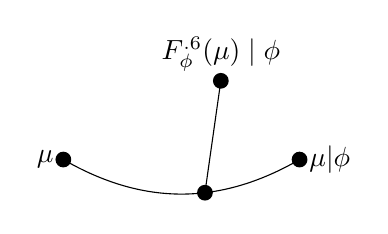
\begin{tikzpicture}
        \coordinate[label=left:$\mu$] (A) at (0,0);
        \coordinate[label=right:$\mu|\phi$] (C) at (3,0);
        \coordinate[label=above:$F_\phi^{.6}(\mu)\mid\phi$] (C') at (2,1);
        \draw (A) to[bend right] node[outer sep=0,pos=0.6](B){} (C);
        \fill 
            (A) circle (0.1)
            (B) circle (0.1)
            (C) circle (0.1)
            (C') circle (0.1);
        \draw (B.center) to (C');
    \end{tikzpicture}
    \end{center}


    \subsection{Halting Updates (Dropping \ref{ax:nopause})}
    The next two examples further explore the motivation behind \cref{ax:nopause}

    \begin{example}
    Suppose $\Theta = \mathbb R \cup \{-\infty, \infty\}$, $\Phi = \{\star\}$ is a singleton, and
    and 
    \[
        F^t_{\!\star}(\theta) = \theta + t + \sin(t).
    \]

    This is interesting because it ``pauses'' 
    Clearly $F$ satisfies \cref{ax:zero,ax:idemp,ax:cont,ax:diffble}.
    It also satisfies \cref{ax:seq-for-more}, since it is increasing in $t$
    (but it is not additive \cref{ax:additivity}).
    %
    Its vector field is given by 
    \[
        \frac{\partial}{\partial t} F^t_{\!\star}(\theta) = 1 + \cos(t) \Big|_{t=0}
         = 2,
    \]
    so its unique additive representation is
    $
        {^+}F^t_{\!\star}(\theta) = \theta + 2 t.
    $
    \end{example}

    \begin{example}
    Now suppose $\Theta$ and $\Phi$ are as before,
    but now
    \[
        F^t_{\!\star}(\theta) = \theta + t - \sin(t).
    \]
    As before, it satisfies \cref{ax:zero,ax:idemp,ax:cont,ax:diffble,ax:seq-for-more},
    but now its vector field is
    \[
        \frac{\partial}{\partial t} F^t_{\!\star}(\theta) = 1 - \cos(t) \Big|_{t=0}
         = 0,
    \]
    so its unique additive representation does nothing:
    $
        {^+}F^t_{\!\star}(\theta) = \theta. 
    $
    \end{example}

    \subsection{}




    \section{Extra Properties of Update Rules}

    \subsection{Invertable Update Rules}

    \begin{LrnAxioms}
    	\item For all $\phi\in\Phi$, and $\beta \in \mathbb R$, the update
    	$F^{\beta}_{\phi}: \Theta \to \Theta$ is invertable.
    	\hfill\textbf{(Invertability)} \label{ax:invert}
    \end{LrnAxioms}


    This effectively partitions $\Theta$ into two


    \begin{prop}
    	If $F$ is a differentiable and invertable update rule (i.e., satisfies \cref{ax:zero,ax:additivity,ax:invert,ax:diffble}), then for all $\beta \in \mathbb R$, $\phi \in \Phi$, the function
    	% $F^\beta_\phi : \Delta\X \to \Delta\X$
    	$F^\beta_\phi : \Theta \to \Theta$
    	is a diffeomorphism, and its inverse is given by $F^{-\beta}_\phi$, in the sense that
    	\[
    		F^{-\beta}_\phi( F^{\beta}_\phi (\mu) ) = \mu = F^{\beta}_\phi( F^{-\beta}_\phi (\mu) ).
    	 \]
    \end{prop}


    % Together with strong additivity, we get
    % \begin{prop% We are primarily interested in the case where confidence can be measured as a real number,
    %     If $F$ is an update rule satisfying \cref{ax:additivity,ax:invert},
    %     then any update prescribed by $F$ (or sequence thereof) takes positive distributions to positive distributions.
    %     %
    %     Concretely, for all $\beta$ and $\phi$,   $\mu \in \mathrm{Int}(\Delta\X)$ if and only if $F^{\beta}_\phi(\mu) \in \mathrm{Int}(\Delta\X)$.
    %     If $F$ further satisfies \cref{ax:sufficiency, ax:diffble}, then
    %     % \[
    %         $F^\beta_\phi$ is a diffemorphism of $\mathrm{Int}(\Delta\X)$.
    %     % \]
    % \end{prop}


    As a consequence,
    \begin{coro}
    	If for any $\beta < \infty$ there exist $\mu, \phi, A$ such that
    	$\mu(A) > 0$  but $F^{\beta}_\phi(\mu)(A) = 0$, then $F$ is not invertable.
    \end{coro}


    \subsection{Truth}
    % We have seen how idempotence seems to be a feature of full-confidence updates. 
    Implicit in a full-confidence update rule is a notion of truth:
    given a full-confidence update rule $F^\top$, we define
    a binary relation ${\models_{F^\top}} \subseteq \Phi \times \Theta$ 
    between belief states and propositions, by 
    $\theta \models_{F^\top} \phi$
    (read: $\phi$ is true in $\theta$)
    iff $F^\top_\phi(\theta) = \theta$.
    %
    It is easy to verify that in our previous examples,
    this gives the appropriate notion of truth.

    \begin{itemize}
    	\item \textbf{Conditioning.}
    	$\mu \models_{(|)} \phi \iff \mu(\phi) = 1$.
    	% {\color{red}%
    	% or $\mu(\phi) = 0$. 
    	% }
    	\item \textbf{Imaging.}
    	For $w \in W$, $w \models_f \phi$ iff $\phi$ is true in $w$. 
    	Meanwhile, $\mu \models \phi \iff \mu(\phi) = 1$.
    	\item \textbf{Jeffrey's Rule.}
    	$\mu \models_J \pi(X) \iff \mu_X = \pi$.
    	That is, if the marginal of $\mu$ on the variable $X$ equals $\pi$. 
    \end{itemize}


    \subsection{Enriching Belief Space to Track Confidence}

    \begin{example}\label{ex:dupl-enriched}
    Suppose $F$ is an additve update rule. Then, we can explicitly construct a resolution to the problem posed in \cref{ex:dupl} by defining enriched spaces
    \begin{align*}
    	\Phi' &:= \Phi \times \Big\{ \text{ identities }~ \mathit{id}~ \Big\}\\
    	\Theta' &:= \Theta \times
    		\Big\{ \text{histories } L = [(\phi_1, \mathit{id}_1, c_1), \ldots (\phi_n, \mathit{id}_n, c_n)] \Big\} \\
    \end{align*}
    and new commitment function\ $G$ by
    \begin{align*}
    	 G^{\beta}_{(\phi,\mathit{id})}(\theta, L) & :=
    		\begin{cases}
    		\Big( F^{\beta- \sum_{i}\beta_i \mathbbm1[(\phi_i,\mathrm{id}_i) = (\phi, \mathrm{id})]}_{\phi}(\theta),~
    			 L :: (\phi,\mathit{id}, \beta)
    		 \Big)
    			 &\text{ if } \beta \ne \bot \\
    		(\theta, L) &
    			   \text{ if } \beta = \bot
    	\end{cases}
    \end{align*}
    \end{example}


    \subsection{More on Path Update Rules}
    Since each $\phi$ corresponds to a path

    \begin{defn}[Homotopic update rules]
    	$\phi \sim_F \psi$  iff 
    	they behave the same way for full confidence (that is, 
    	$F^1_{\phi}(\theta) = F^1_{\psi}(\theta)$ for all $\theta \in \Theta$)
    	and  there exists a continuous function
    	$H : \Theta \times [0,1] \times [0,1]$ such that,
    	for all $\theta \in \Theta$ and $\chi \in [0,1]$,
    	\begin{enumerate}[nosep]
    		\item $H(\theta, \chi, 0)= F(\theta, \chi, \phi)$,
    		\item $H(\theta, \chi, 1)= F(\theta, \chi, \psi)$
    	\end{enumerate}
    	and for all $s \in [0,1]$,
    	\begin{enumerate}[nosep,resume]
    		\item $H(\theta, 0, s) = \theta$;
    		\item $H(\theta, 1, s) = F^1_{\phi}(\theta) = F^1_{\psi}(\theta)$,
    		the last two of	which are the same by assumption. \qedhere
    	\end{enumerate}
    \end{defn}

    As usual, homotopy is an equivalence relation.

    For example, the Dempster-Shafer update rule \eqref{eq:ds-prob} is homotopic 
    to the linear update rule from \cref{ex:prob-simple}. 

    \subsection{Linear Update Rules}

    % In some sense, ALL update rules are linear in $\bar\Phi$ by definition.

    There are many definitions of linear update rules:
    \begin{defn}\label{ax:linear}
    Let $F$ be a differentiable update rule on $\Theta$. We say that $F$ is \textellipsis
    \begin{itemize}
    \item \emph{linear} if $\Theta$ is a vector space over $\mathbb R$, and the
    vector field $F'_\phi$ is a linear operator, i.e., for all $a, b \in \mathbb R$, we have that
    \[ F'_\phi(a \theta_1 + b \theta_2) = a F'_\phi(\theta_1) + b F'_\phi(\theta_2). \]

    \item \emph{cvx-linear} if $\Theta \subset \mathbb R^n$ is a convex set, and, for all $a \in [0,1]$, we have that
    \[ F'_\phi(a \theta_1 + (1-a) \theta_2) = a F'_\phi(\theta_1) + (1-a) F'_\phi(\theta_2). \]

    \item \emph{$\mathcal L$-cvx-linear} if $\Theta \subset \mathbb R^n$ and $F$ is an optimizing update rule with a loss representation $\mathcal L$ linear in its first argument, i.e.,
    \[
        \mathcal L(a \theta_1 + (1-a) \theta_2, \varphi) = a \mathcal L(\theta_1, \varphi) + (1-a) \mathcal L(\theta_2, \theta).
    \]
    \end{itemize}
    % $F'_\phi(\theta) = \mathrm{V}_\phi \theta$ for some linear operator $V_\phi \in \mathbb R^{n \times n}$.
    % $F'_\phi(\theta) = \mathrm{V}_\phi \theta$ for some linear operator $V_\phi$.
    \end{defn}

    \begin{prop}
    If $F$ is a $\mathcal L$-cvx-linear, then it is also cvx-linear.
    \end{prop}

    In fact, the first condition is much stronger;
    \begin{prop}
    if $F$ is a nontrivial $\mathcal L$-cvx-linear optimizing UR, then $\Theta$ equals cone generated by  the rays $\{ F'_\varphi\theta : \theta \in \Theta, \varphi \in \Phi \}$. In particular, if there is some $\theta$ such that $0$ is in the interior of the convex hull $\mathrm{conv}(\{F'_\phi\theta\}_{\phi \in \Phi})$, then $\Theta = \mathbb R^n$.
    \end{prop}

    % Implicit in this definition is the supposition that the integral curves generated by the differential equations, started at any point $\theta \in \Theta$, are

    \begin{prop}
    % If $F$ is a  differ
    Every linear update rule is of the form
    $
        F^{\beta}_\phi(\theta) =  \theta^{T} \exp(\beta V)
    $,
    where $\exp(\beta V)$ is the matrix exponential.%
        \footnote{Concretely, if $V = U^T \mathrm{Diag}(\lambda_1, \ldots \lambda_n) U$ is an eigendecomposition of $V$, then $\exp(V) = U^T \mathrm{Diag}(e^{\beta\lambda_1}, \ldots e^{\beta\lambda_n}) U$.}
    \end{prop}

    \begin{prop}
    A linear update rule $F$ is commutative iff, for every pair of statements  $\phi, \phi' \in \Phi$, the
    matrices $V_\phi$ and $V_{\phi'}$ commute.
    \end{prop}




    \clearpage
    \section{Proofs}

    \begin{linked}{prop}{synthetic-bel}
    	For every learner $\Lrn$, there exists a 
    	believer $\Bel$ such that the pair $(\Lrn, \Bel)$ satisfy 
    	\cref{ax:monotone,ax:truth-is-enough,ax:effectiveness}
    \end{linked}
    % \recall{prop:synthetic-bel}
    \begin{lproof}\label{proof:synthetic-bel}
    	Given $\Lrn: \Phi \times \confdom \times \Theta \to \Theta$,
    	define 
    	\[
    	\Bel(\theta,\phi) := 
    	\begin{cases}
    		\top & \text{ if } \exists \chi.~\Lrn(\phi,\chi,\theta) = \theta \\
    		\bot & \text{ otherwise } 
    	\end{cases}
    	\]
    \end{lproof}


    \recall{theorem:add-reparam}
    \begin{lproof}\label{proof:add-reparam}
        
    	
    \end{lproof}



    \recall{prop:bolz-props}
    \begin{lproof}\label{proof:bolz-props}
    	\textbf{Commutativity.}
    	For some normalization factors $Z, Z', Z''$, we have:
    	\begin{align*}
    		 F^\beta_\phi( F^{\beta'}_{\phi'}(\mu))
    		 &= F^\beta_\phi \Big( \frac{1}{Z} \,\mu\, \exp(- \beta' c_{\phi'}) \Big) \\
    		 &= \frac{1}{Z'} \frac{1}{Z} \,\mu\, \exp(- \beta' c_{\phi'}) \exp(- \beta c_{\phi}) \\
    		 &= \frac{1}{Z''} \,\mu\, \exp(-\beta' c_{\phi'} - \beta c_\phi)
    	\end{align*}
    	which is the same expression when we exchange $(\phi, \beta)$ and $(\phi', \beta')$.
    \end{lproof}

    \recall{prop:bolz-fields}
    \begin{lproof}\label{proof:bolz-fields}
    	Let $f(X) := \exp(-\beta U(X,\varphi))$, and $g(X) := U(X,\varphi)$.
    	\begin{align*}
    		\mathrm{Boltz}'_\varphi\theta &= \frac{\partial}{\partial \beta} \mathrm{Boltz}^\beta_\varphi(p) \Big|_{\beta=0} \\
    	\intertext{\TODO[TODO: finish typesetting algebra]}
    		&= x \mapsto
    			p(x) \frac{f(x)}{\Ex_p[f]}
    				\left(\Ex_p\left[ \frac{f}{\Ex_{p}[f]} g\right] - g(x) \right)
    				% {\exp(-\beta U(x,\varphi))}
    				% {\Ex_{}}
    				\Big|_{\beta=0}
    				\\
    		&= \frac{pf}{\Ex_p[f]^2}
    			\left(\Ex\nolimits_p\left[ f g\right] - g \Ex\nolimits_{p}[f] \right)
    			\Big|_{\beta=0} \\
    		&= x \mapsto p(x) (\Ex\nolimits_p[g] - g(x)) &
    			\text{since $f(X) = 1$ when $\beta=0$}
    	\end{align*}
    	As a sanity check, note that the sum over all components is
    	\[ \sum_{x \in X} ((\mathrm{Boltz}\,U)'_\varphi\, \theta)_x
    		 = \sum_{x \in X} p(x) (\Ex\nolimits_p[g] - g(x))
    		 = \Ex\nolimits_p[ \Ex\nolimits_p [ g ]] - \Ex\nolimits_p [g] = 0,
    	 \]
    	 so indeed it lies within the tangent space.
    \end{lproof}
\end{subappendices}
